% !TEX program = xelatex
\documentclass[UTF8,fontset=fandol,a4paper,11pt]{ctexart}
\usepackage[margin=21mm,top=23mm,bottom=22mm,headheight=16pt]{geometry}
\usepackage{amsmath,amssymb,mathtools,bm}
\usepackage{tikz}
\usetikzlibrary{arrows.meta,calc,angles,quotes,patterns,decorations.pathmorphing}
\usepackage{xcolor,booktabs,array,longtable,enumitem,fancyhdr,needspace}
\usepackage[unicode,hidelinks]{hyperref}
\definecolor{ink}{HTML}{24343C}
\definecolor{accent}{HTML}{166A70}
\definecolor{muted}{HTML}{65747A}
\definecolor{rulegray}{HTML}{D4DDE0}
\definecolor{warm}{HTML}{966037}
\color{ink}
\setlength{\parindent}{2em}
\setlength{\parskip}{4pt}
\linespread{1.12}
\AtBeginDocument{\setlength{\abovedisplayskip}{6pt plus 2pt minus 1pt}
\setlength{\belowdisplayskip}{6pt plus 2pt minus 1pt}
\setlength{\abovedisplayshortskip}{0pt plus 1pt}
\setlength{\belowdisplayshortskip}{4pt plus 1pt}}
\setlist[enumerate]{label=(\arabic*),leftmargin=2.3em,itemsep=3pt,topsep=4pt}
\setlist[itemize]{leftmargin=2em,itemsep=2pt,topsep=4pt}
\allowdisplaybreaks[1]
\setlength{\emergencystretch}{2em}
\setcounter{secnumdepth}{0}
\providecommand{\tightlist}{\setlength{\itemsep}{0pt}\setlength{\parskip}{0pt}}
\ctexset{section={format=\Large\bfseries\color{accent},beforeskip=10pt,afterskip=9pt},
subsection={format=\normalsize\bfseries\color{accent},beforeskip=10pt,afterskip=4pt},
subsubsection={format=\normalsize\bfseries,beforeskip=8pt,afterskip=3pt}}
\pagestyle{fancy}
\fancyhf{}
\fancyhead[L]{\small\color{muted}物理学难题集萃}
% 页眉仅保留书名；版本名称只在封面显示。
\fancyfoot[L]{\small\color{muted}\chapterlabel}
\fancyfoot[R]{\small\thepage}
\renewcommand{\headrulewidth}{0.4pt}
\renewcommand{\footrulewidth}{0pt}
\newcommand{\dd}{\mathop{}\!\mathrm{d}}
\newcommand{\vect}[1]{\bm{#1}}
\newcommand{\tagline}[1]{\noindent{\small\color{muted}#1}\par}
\newcommand{\result}[1]{\begin{equation*}\boxed{#1}\end{equation*}}
\newcommand{\figcaption}[1]{\par\vspace{2pt}{\small\color{muted}#1}\par}
\newcommand{\teach}[2]{\Needspace{4\baselineskip}\subsection*{讲解要点与追问}#1\par\smallskip\noindent\textbf{追问：}#2\par}
\newcommand{\workarea}{\par\vspace{7mm}\noindent{\small\color{muted}作答区}\par\vspace{4mm}
\noindent\textcolor{rulegray}{\rule{\linewidth}{0.3pt}}\par\vspace{16mm}
\noindent\textcolor{rulegray}{\rule{\linewidth}{0.3pt}}\par\vspace{16mm}
\noindent\textcolor{rulegray}{\rule{\linewidth}{0.3pt}}\par\vspace{16mm}
\noindent\textcolor{rulegray}{\rule{\linewidth}{0.3pt}}}
\tikzset{axis/.style={-{Stealth[length=2mm]},thin,color=muted},
motion/.style={-{Stealth[length=2.3mm]},thick,color=accent},
force/.style={-{Stealth[length=2.3mm]},thick,color=warm},
traj/.style={thick,color=accent},guide/.style={dashed,thin,color=muted},
object/.style={thick,color=ink},every node/.style={font=\small}}\widowpenalty=10000\clubpenalty=10000\displaywidowpenalty=10000

\newcommand{\chapterlabel}{第四章\quad 角动量与有心运动}
\hypersetup{pdftitle={第四章 角动量与有心运动·教师版},pdfauthor={},pdfsubject={第四章第1--14题}}
\begin{document}
\pdfbookmark[0]{第四章 角动量与有心运动}{cover}
\thispagestyle{empty}
\vspace*{20mm}
\noindent{\Huge\bfseries 物理学难题集萃}\par\vspace{8mm}
\noindent{\LARGE 第四章\quad 角动量与有心运动}\par\vspace{10mm}
\noindent{\Large\color{accent}教师版}\par\vspace{8mm}
\noindent\textcolor{accent}{\rule{\linewidth}{1pt}}\par\vspace{8mm}
\noindent 第 1--14 题\par\vspace{5mm}
\noindent 详细解答、备课分析、课堂追问与变式训练。\par
\vfill\clearpage
\pdfbookmark[1]{题目目录}{contents}
\section*{题目目录}
\begin{longtable}{@{}>{\color{accent}\bfseries}r p{120mm}@{}}
\toprule 题号 & 题目\\\midrule
1 & 万有引力推出开普勒三定律 \\
2 & 椭圆轨道反推平方反比引力 \\
3 & 初速度决定有心轨道类型 \\
4 & 两质点万有引力相碰时间 \\
5 & 绕月飞船两种登月喷气方案 \\
6 & 圆轨道径向脉冲后的近远地点 \\
7 & 椭圆轨道发射探测器后的轨道 \\
8 & 彗星抛物线轨道与地球轨道交点 \\
9 & 宇航站发射飞船后的再次相遇 \\
10 & 地火霍曼转移轨道 \\
11 & 火星圆轨道径向微扰后的椭圆轨道 \\
12 & 借助火星引力弹弓逃离太阳系 \\
13 & 弹簧有心力场中的有效势能曲线 \\
14 & 均匀宇宙尘埃中的圆形行星轨道 \\
\bottomrule\end{longtable}


\clearpage

\pdfbookmark[2]{第 1 题 万有引力推出开普勒三定律}{q1}

\section*{第 1 题\quad 万有引力推出开普勒三定律}

\tagline{M-04-01}

设太阳质量为 $M$，行星质量为 $m\ll M$，忽略其他天体的作用，将太阳视为固定。行星所受引力为
\[
\vect F=-\frac{GMm}{r^2}\vect e_r.
\]
根据牛顿万有引力定律证明开普勒行星运动三定律：束缚的非径向轨道为椭圆，太阳位于一个焦点；径矢的面积速度恒定；绕同一太阳运动的行星满足 $T^2/a^3$ 为常量。这里 $a$ 为半长轴，$T$ 为周期。说明束缚条件与非束缚轨道的区别。

\par\medskip\noindent\begin{minipage}{\linewidth}\centering
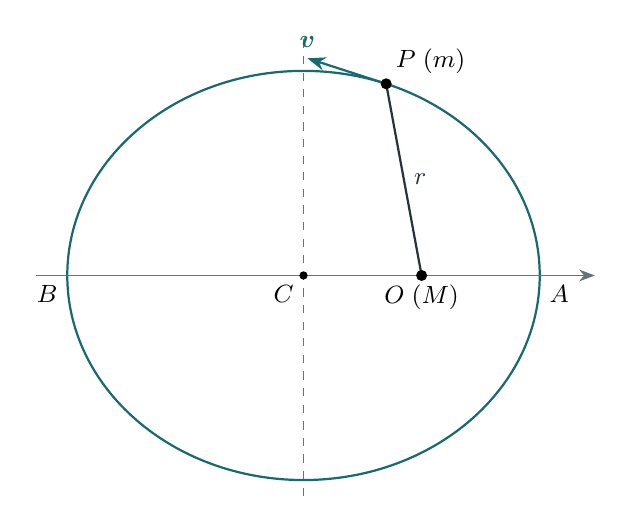
\begin{tikzpicture}[scale=1]
\draw[traj] (0.0000,0.0000) ellipse (3.0000 and 2.5981);

\coordinate (O) at (1.5,0);\coordinate (C) at (0,0);
\coordinate (P) at (1.05,2.434);\coordinate (A) at (3,0);\coordinate (B) at (-3,0);
\draw[axis] (-3.4,0)--(3.7,0);\draw[guide] (0,-2.8)--(0,3.0);
\draw[object] (O)--(P) node[midway,right] {$r$};
\draw[motion] (P)--++(-1.0,.324) node[above] {$\vect v$};
\fill (O) circle (2pt) node[below] {$O\;(M)$};\fill (C) circle (1.5pt) node[below left] {$C$};
\fill (P) circle (2pt) node[above right] {$P\;(m)$};
\node[below right] at (A) {$A$};\node[below left] at (B) {$B$};

\end{tikzpicture}
\figcaption{图 4.1　太阳位于焦点 $O$，椭圆中心为 $C$。}
\end{minipage}\par\medskip

\Needspace{5\baselineskip}

\pdfbookmark[3]{题型定位}{q1-h0}

\subsection*{题型定位}

平方反比有心力的总纲证明题。先建立平面运动、角动量与能量守恒，再推出圆锥曲线；用负能量条件筛选行星的束缚椭圆。面积定律由零力矩给出，周期律再把椭圆面积与两拱点的速度关系相连。

本题得到的
\(p=h^2/\mu\)、\(e^2=1+2\varepsilon h^2/\mu^2\)、\(T=2\pi\sqrt{a^3/\mu}\)，将用于后续轨道分类、变轨、拱点与飞行时间计算。讲解应明确每个公式的守恒量及适用条件。

\Needspace{5\baselineskip}

\pdfbookmark[3]{知识点}{q1-h1}

\subsection*{知识点}

\begin{itemize}
\tightlist
\item
  平方反比有心力
\item
  极坐标运动方程
\item
  角动量守恒与面积速度
\item
  机械能与圆锥曲线
\item
  开普勒第三定律
\end{itemize}

平方反比中心力保证角动量守恒，从而给面积速度不变。轨道微分方程给以引力中心为焦点的圆锥曲线，负能量时为椭圆。周期由椭圆面积除面积速度得到，同一中心天体的常量在忽略行星质量时才与行星质量无关。


\Needspace{5\baselineskip}

\pdfbookmark[3]{物理图像}{q1-h2}

\subsection*{物理图像}

太阳在焦点，行星的径矢不断扫过面积。由于引力始终沿径向，太阳对行星的力矩为零，所以角动量方向固定，运动限制在一个平面内。

将平方反比引力代入径向运动方程，得到以太阳为焦点的圆锥曲线。非零角动量下，负、零、正比能量依次对应椭圆、抛物线和双曲线。行星束缚于太阳，取负能量的椭圆分支。

解图4.1B以太阳所在焦点为面积顶点，解图4.1C标出长轴两端的速度。椭圆中心$C$与力心$O$的位置不同，写$r$时始终指$O$到行星的距离；解图4.1D再把两拱点对应到有效势曲线的两个交点。

\Needspace{5\baselineskip}

\pdfbookmark[3]{解题入口}{q1-h3}

\subsection*{解题入口}

先在解图4.1B 写出 $h=r^2\dot\varphi$ 和面积速度 $h/2$。将径向运动方程中的时间导数改成对 $\varphi$ 求导，得到 $u=1/r$ 的线性方程。再由轨道参数求半长轴、半短轴，椭圆总面积除以面积速度得到周期。负能量轨道的允许半径由解图4.1D 的两个交点确定。

\Needspace{5\baselineskip}

\pdfbookmark[3]{标准解法}{q1-h4}

\subsection*{标准解法}

\subsubsection*{平面运动与守恒量}
取太阳为原点，记 $\mu=GM$。引力的力矩为零：
\[
\frac{\dd\vect L}{\dd t}=\vect r\times\vect F=0,
\qquad \vect L=m\vect r\times\vect v.
\]
当 $L\ne0$ 时，$\vect r$ 始终垂直于固定的 $\vect L$，因此运动在一个固定平面内。$L=0$ 时，行星沿经过太阳的直线运动，时间演化直接由径向能量式求出。后面的极角变量取 $L\ne0$ 的平面运动。

\par\medskip\noindent\begin{minipage}{\linewidth}\centering
\begin{tikzpicture}[scale=1]

\coordinate (O) at (0,0);\coordinate (P) at (3,1.6);
\draw[axis] (-.3,0)--(4.8,0) node[right] {极轴};
\draw[object] (O)--(P) node[midway,above] {$r$};
\draw[guide] (P)--(4.4,2.347);
\draw[motion] (P)--(3.9,2.08) node[above right] {$\dot r\,\vect e_r$};
\draw[motion] (3.9,2.08)--(3.33,3.15) node[right] {$r\dot\varphi\,\vect e_\varphi$};
\draw[motion] (P)--(3.33,3.15) node[left] {$\vect v$};
\draw[force] (P)--(1.9,1.013) node[below right] {$\vect F$};
\draw[muted] (.65,0) arc (0:28.072:.65) node[midway,right] {$\varphi$};
\fill (O) circle (2pt) node[below] {$O$};\fill (P) circle (2pt) node[below right] {$P$};

\end{tikzpicture}
\figcaption{解图 4.1A　同一点的径向、横向速度与引力。}
\end{minipage}\par\medskip

解图 4.1A 的两个基矢随极角转动，满足
\[
\dot{\vect e}_r=\dot\varphi\vect e_\varphi,
\qquad \dot{\vect e}_\varphi=-\dot\varphi\vect e_r.
\]
对 $\vect r=r\vect e_r$ 求导，得到
\[
\begin{aligned}
\vect v&=\dot r\vect e_r+r\dot\varphi\vect e_\varphi,\\
\vect a&=(\ddot r-r\dot\varphi^2)\vect e_r
 +(r\ddot\varphi+2\dot r\dot\varphi)\vect e_\varphi.
\end{aligned}
\]
于是角动量和机械能可写为
\[
h\equiv\frac Lm=r^2\dot\varphi,\qquad
\varepsilon\equiv\frac Em
=\frac12\dot r^2+\frac{h^2}{2r^2}-\frac\mu r.
\]
这里 $h$ 为比角动量，$\varepsilon$ 为比能量；无穷远处引力势能取零。

\subsubsection*{轨道方程与第一定律}
令 $u=1/r$，以撇号表示对 $\varphi$ 求导。利用 $\dot\varphi=hu^2$，有
\[
\dot r=\frac{\dd r}{\dd\varphi}\dot\varphi=-hu',
\qquad \ddot r=-h^2u^2u''.
\]
径向动力学方程是
\[
\ddot r-r\dot\varphi^2=-\frac\mu{r^2}.
\]
将上式代入，并注意 $r\dot\varphi^2=h^2u^3$，得到
\[
-h^2u^2(u''+u)=-\mu u^2,
\qquad u''+u=\frac\mu{h^2}.
\]
特解为 $\mu/h^2$，齐次解为 $A\cos\varphi+B\sin\varphi$。将极轴选在近点方向，可使 $B=0$、$A\geq0$。令
\[
p=\frac{h^2}\mu,\qquad A=\frac ep,
\]
得到
\[
u=\frac{1+e\cos\varphi}p,
\qquad \boxed{r=\frac p{1+e\cos\varphi}}.
\]
这是以 $O$ 为焦点的圆锥曲线。$p$ 为半通径：$\varphi=\pi/2$ 时 $r=p$；$e$ 为离心率。按焦点、准线定义，$e$ 等于点到焦点的距离与点到准线距离之比。

也可直接从能量推导。将 $\dot r=-hu'$ 代入能量式，得到
\[
(u')^2+u^2-\frac{2\mu}{h^2}u=\frac{2\varepsilon}{h^2}.
\]
对 $\varphi$ 求导得 $2u'(u''+u-\mu/h^2)=0$。在 $u'\ne0$ 的区间约去 $u'$，再以连续性延伸到孤立拱点。圆轨道有 $u'\equiv0$，直接由径向力等于圆周运动向心需求求半径。

把轨道解代回能量式，$u'=-(e/p)\sin\varphi$，所以
\[
\begin{aligned}
\frac{2\varepsilon}{h^2}
&=\frac{e^2\sin^2\varphi+(1+e\cos\varphi)^2
 -2(1+e\cos\varphi)}{p^2}\\
&=\frac{e^2-1}{p^2}.
\end{aligned}
\]
因 $p=h^2/\mu$，故
\[
\boxed{e^2=1+\frac{2\varepsilon h^2}{\mu^2}
=1+\frac{2EL^2}{G^2M^2m^3}}.
\]
对物理上允许且 $h\ne0$ 的初始状态，$\varepsilon<0$ 对应 $0\leq e<1$ 的椭圆，$e=0$ 为圆；$\varepsilon=0$ 对应抛物线，$\varepsilon>0$ 对应双曲线。行星束缚于太阳，故第一定律适用于负能量轨道。抛物线在 $\varphi\to\pi$ 时半径趋于无穷；双曲线的无穷远方向在 $\varphi=\arccos(-1/e)$。因此两者都没有有限远日点。

\subsubsection*{面积速度与第二定律}
\par\medskip\noindent\begin{minipage}{\linewidth}\centering
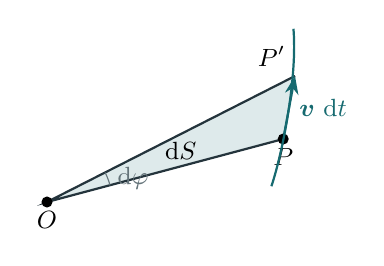
\begin{tikzpicture}[scale=1]

\coordinate (O) at (0,0);\coordinate (P) at (3,.8);\coordinate (Q) at (3.15,1.6);
\fill[accent!14] (O)--(P)--(Q)--cycle;
\draw[object] (P)--(O)--(Q);\draw[motion] (P)--(Q) node[midway,right] {$\vect v\,\dd t$};
\node at (1.7,.65) {$\dd S$};\node[above left] at (Q) {$P'$};
\fill (O) circle (2pt) node[below] {$O$};\fill (P) circle (2pt) node[below] {$P$};
\draw[traj] (2.85,.2) .. controls (3,.65) and (3.18,1.6) .. (3.13,2.2);
\draw[muted] (.8,.213) arc (14.931:26.926:.828) node[midway,right] {$\dd\varphi$};

\end{tikzpicture}
\figcaption{解图 4.1B　径矢扫过的微元面积。}
\end{minipage}\par\medskip

解图 4.1B 中 $P\to P'$ 的位移为 $\vect v\,\dd t$，扫面积矢量为
\[
\dd\vect S=\frac12\vect r\times\dd\vect r,
\qquad \frac{\dd\vect S}{\dd t}=\frac12\vect r\times\vect v
=\frac{\vect L}{2m}.
\]
方向固定且大小恒定，因此
\[
\boxed{\frac{\dd S}{\dd t}=\frac h2
=\frac12r^2\dot\varphi=\text{常量}}.
\]
一般位置只有横向速度 $v_\varphi$ 贡献面积速度：$rv\sin\gamma=h$，$\gamma$ 为径矢与速度的夹角。近、远日点速度垂直于径矢，因而 $r_Av_A=r_Bv_B=h$。面积速度恒定，行星速率随轨道位置变化。

\subsubsection*{椭圆几何与第三定律}
\par\medskip\noindent\begin{minipage}{\linewidth}\centering
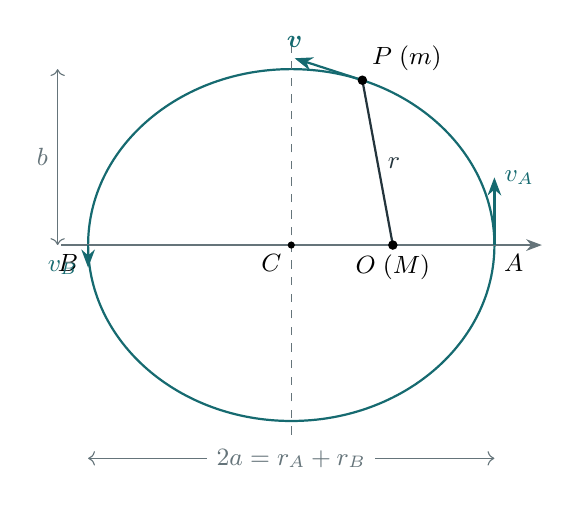
\begin{tikzpicture}[scale=0.86]
\draw[traj] (0.0000,0.0000) ellipse (3.0000 and 2.5981);

\coordinate (O) at (1.5,0);\coordinate (C) at (0,0);
\coordinate (P) at (1.05,2.434);\coordinate (A) at (3,0);\coordinate (B) at (-3,0);
\draw[axis] (-3.4,0)--(3.7,0);\draw[guide] (0,-2.8)--(0,3.0);
\draw[object] (O)--(P) node[midway,right] {$r$};
\draw[motion] (P)--++(-1.0,.324) node[above] {$\vect v$};
\fill (O) circle (2pt) node[below] {$O\;(M)$};\fill (C) circle (1.5pt) node[below left] {$C$};
\fill (P) circle (2pt) node[above right] {$P\;(m)$};
\node[below right] at (A) {$A$};\node[below left] at (B) {$B$};
\draw[<->,muted] (-3,-3.15)--(3,-3.15) node[midway,fill=white] {$2a=r_A+r_B$};
\draw[<->,muted] (-3.45,0)--(-3.45,2.598) node[midway,left] {$b$};
\draw[motion] (A)--++(0,1) node[right] {$v_A$};\draw[motion] (B)--++(0,-.333333) node[left] {$v_B$};
\end{tikzpicture}
\figcaption{解图 4.1C　近、远日点与椭圆的几何参数。}
\end{minipage}\par\medskip

解图 4.1C 中 $C$ 是椭圆中心，$O$ 是焦点。令焦距 $CO=c=ae$，有
\[
r_A=a-c,\quad r_B=a+c,\quad
r_A+r_B=2a,\quad r_Ar_B=a^2-c^2=b^2.
\]
\Needspace{17\baselineskip}
在两个拱点列能量与角动量关系：
\[
\frac12v_A^2-\frac\mu{r_A}
=\frac12v_B^2-\frac\mu{r_B},\qquad
v_B=\frac{r_A}{r_B}v_A.
\]
非圆椭圆 $r_A\ne r_B$ 时，代入、约去 $r_B-r_A$，得到
\[
v_A^2\left(1-\frac{r_A^2}{r_B^2}\right)
=2\mu\left(\frac1{r_A}-\frac1{r_B}\right),
\qquad v_A^2=\frac{2\mu r_B}{r_A(r_A+r_B)}
=\frac\mu a\frac{r_B}{r_A}.
\]
因此 $h=r_Av_A=b\sqrt{\mu/a}$，代回拱点能量还可得到 $\varepsilon=-\mu/(2a)$。对于圆轨道，直接用 $v^2=\mu/a$ 可得到相同关系。

一周扫过整个椭圆，面积为 $\pi ab$。由第二定律，
\[
T=\frac{\pi ab}{h/2}
=\frac{2\pi a^{3/2}}{\sqrt\mu},
\qquad \boxed{\frac{T^2}{a^3}=\frac{4\pi^2}{GM}}.
\]
同一太阳的 $M$ 相同，右端不依赖行星的 $m$ 或偏心率。若不忽略行星质量，两体相对轨道的引力参数应为 $G(M+m)$；本题的共同常量建立在 $m\ll M$ 的近似下。
\subsubsection*{从极坐标方程逐项识别椭圆参数}
以下直角坐标$(X,Y)$以焦点$O$为原点，正$X$方向指向近点$A$。
轨道方程$r(1+e\cos\varphi)=p$给出
\[
\sqrt{X^2+Y^2}+eX=p.
\]
对椭圆$0\leq e<1$，移项平方并整理：
\[
(1-e^2)X^2+Y^2+2peX-p^2=0,
\]
\[
\frac{[X+pe/(1-e^2)]^2}{p^2/(1-e^2)^2}
+\frac{Y^2}{p^2/(1-e^2)}=1.
\]
因此半长轴与半短轴分别是
\[
a=\frac p{1-e^2},\qquad b=\frac p{\sqrt{1-e^2}},\qquad
c=\sqrt{a^2-b^2}=ae.
\]
中心在$X=-ae$，而$O$恰距中心$ae$，所以$O$确实是焦点。
解图4.1C把中心画在纸面坐标原点、焦点画在其右侧，与这里以焦点为原点的坐标只相差平移。
半长轴、半通径和焦点到近点的距离分别为$a,p,p/(1+e)$，一般并不相同。
当$e=0$时三者才都等于圆半径。

对于$e>0$，由$r=p-eX=e(p/e-X)$还可直接读出准线$X=p/e$，
即点到焦点的距离等于到准线距离的$e$倍。
这个几何定义中的 $e$ 正是动力学积分给出的离心率。椭圆中心在 $X=-ae$，引力中心仍在焦点 $O$，两者间距为 $ae$。
对非束缚轨道，$r>0$还限制$1+e\cos\varphi>0$：
抛物线的无穷远方向为$\varphi\to\pm\pi$，
双曲线的实际分支为 $|\varphi|<\arccos(-1/e)$，在这个区间内径矢长度为正。到区间端点时半径趋于无穷，$\varphi=\pi$ 在该分支之外。

\subsubsection*{固定角动量时的能量允许范围}
把能量式写成径向的一维形式，定义单位质量有效势能
\[
\varepsilon=\frac12\dot r^2+V_{\rm eff}(r),\qquad
V_{\rm eff}(r)=\frac{h^2}{2r^2}-\frac\mu r.
\]
第一项是固定角动量下的横向动能。消去横向速度以后，它与引力势能一起进入径向能量方程。
对$r$求导，
\[
V'_{\rm eff}=-\frac{h^2}{r^3}+\frac\mu{r^2},\qquad
r_c=\frac{h^2}\mu=p,
\]
\[
V''_{\rm eff}(p)=\frac\mu{p^3}>0,\qquad
V_{{\rm eff},\min}=-\frac\mu{2p}=-\frac{\mu^2}{2h^2}.
\]
径向动能非负，所以比能量位于有效势的最低值以上，满足 $\varepsilon\geq-\mu^2/(2h^2)$。
等号时只能停在有效势阱底，径向速度为零，轨道为圆；
高于此下限而仍为负能量时，存在两个径向转折点，对应椭圆的近点和远点。
解图4.1D的负能量水平线只在两个交点之间允许运动。
零能量及正能量只保留内侧转折点，向外没有有限远点，可以到达无穷远。
\begin{center}\begin{minipage}{\linewidth}\centering
\begin{tikzpicture}[x=1.6cm,y=1.6cm]
\draw[axis](.3,0)--(4.4,0)node[right]{$r/p$};
\draw[axis](.38,-.7)--(.38,1.4)node[above]{$V_{\rm eff}/(\mu/p)$};
\draw[traj,domain=.36:4.1,samples=120]plot(\x,{.5/\x^2-1/\x});
\draw[guide](.45,-.45)--(3.8,-.45);\draw[guide](.45,.25)--(3.8,.25);
\fill(.759746927,-.45)circle(1.7pt);\fill(1.462475296,-.45)circle(1.7pt);
\fill(1,-.5)circle(1.7pt);\node[below]at(1,-.5){圆轨道};
\node[right]at(3.8,-.45){$\varepsilon<0$};\node[right]at(3.8,.25){$\varepsilon>0$};
\node[above]at(3.1,0){$\varepsilon=0$};
\end{tikzpicture}
\figcaption{解图4.1D\quad 固定非零角动量的有效势阱；圆轨道是最低允许能量状态。}
\end{minipage}\end{center}
这也补足$e^2=1+2\varepsilon h^2/\mu^2$中的实数条件。
固定 $h$ 后，径向动能非负把比能量限制在势阱底以上。属于同一允许初态的负能量和非零角动量共同给出束缚椭圆。

由$p=a(1-e^2)$和上述能量关系，进一步得到
\[
\varepsilon=-\frac\mu{2a},\qquad
\boxed{v^2=\mu\left(\frac2r-\frac1a\right)}.
\]
在解图4.1C的两拱点代入$r_A=a(1-e)$、$r_B=a(1+e)$，
\[
v_A^2=\frac\mu a\frac{1+e}{1-e},\qquad
v_B^2=\frac\mu a\frac{1-e}{1+e},\qquad
\frac{v_A}{v_B}=\frac{1+e}{1-e}.
\]
图示$e=1/2$时近点速率为远点的3倍；
此时 $r_B=3r_A$，与角动量关系 $r_Av_A=r_Bv_B$ 给出的反比速率相同。行星从近点向远点运动时速率减小。

\subsubsection*{把面积定律还原为沿椭圆的时间关系}
以近点为计时起点，用恒定的面积速度把行星扫过的面积换成经过各点的时间。
用偏近点角$\psi$参数化同一条椭圆：
\[
X=a(\cos\psi-e),\qquad Y=b\sin\psi,
\qquad r=a(1-e\cos\psi).
\]
$\psi$ 是椭圆的参数角，真近点角 $\varphi$ 则是焦点径矢与近点方向的夹角。后面的时间积分以 $\psi$ 为变量。
由扫面积微元，
\[
\frac{\dd S}{\dd\psi}
=\frac12\left(X\frac{\dd Y}{\dd\psi}-Y\frac{\dd X}{\dd\psi}\right)
=\frac{ab}{2}(1-e\cos\psi).
\]
再除以恒定面积速度$h/2$，利用$h=b\sqrt{\mu/a}$，得到
\[
\frac{\dd t}{\dd\psi}=\sqrt{\frac{a^3}\mu}(1-e\cos\psi).
\]
取经过近点时$t=t_p,\psi=0$，逐项积分为
\[
\boxed{\sqrt{\frac\mu{a^3}}(t-t_p)=\psi-e\sin\psi}.
\]
当$\psi$增加$2\pi$，右端增加$2\pi$，再次得到$T=2\pi\sqrt{a^3/\mu}$。
从 $\psi_1$ 走到 $\psi_2$，时间差由 $\Delta\psi-e\Delta\sin\psi$ 乘以 $\sqrt{a^3/\mu}$ 给出。
非圆椭圆上，同样长的偏近点角区间所扫过的面积取决于区间的位置。例如分别选取近点、远点两侧等宽的角区间，靠近近点时 $1-e\cos\psi$ 较小，扫过这段区间的时间更短。


\Needspace{5\baselineskip}

\pdfbookmark[3]{关键洞察}{q1-h5}

\subsection*{关键洞察}

面积定律只要求合力为有心力；焦点圆锥曲线和 \(T^2\propto a^3\)
则还依赖平方反比。面积速度由角动量守恒确定，焦点圆锥曲线的形状和周期与半长轴的关系还包含径向动力学。

在本题中，能量符号筛选束缚椭圆，角动量给半通径；解图4.1C的
\(r_Ar_B=b^2\) 再把面积速度与半长轴联系起来。求导变换时应保留 \(h\ne0\)
与圆轨道特例。

\Needspace{5\baselineskip}

\pdfbookmark[3]{易错点}{q1-h6}

\subsection*{易错点}

\begin{itemize}
\item 太阳位于焦点 $O$，椭圆的几何中心为 $C$，二者相距 $ae$。
\item 面积速度取 $L/(2m)$。在不同位置，横向速度与半径成反比。
\item 第三定律用完整椭圆面积 $\pi ab$，并用 $h=b\sqrt{\mu/a}$ 消去半短轴。
\item 两拱点满足 $r_Av_A=r_Bv_B$，椭圆的速率随位置改变。
\item 时间导数与角导数通过 $\dot\varphi=hu^2$ 连接。
\item 轨道方程、面积速度和周期分别由径向方程、零力矩和总扫面积求得。
\end{itemize}

\Needspace{5\baselineskip}

\pdfbookmark[3]{课堂讲解建议}{q1-h7}

\subsection*{课堂讲解建议}

在解图4.1A 指出只有横向速度贡献角动量，要求用 $\vect r\times\vect F=0$ 解释面积速度恒定。再让学生按链式法则写出 $\dot r=-hu'$，说明拱点用连续性接上，圆轨道用径向方程单独处理。转到解图4.1C，分别从焦点和中心量出 $r_A,r_B,a,b$，用 $r_Ar_B=b^2$ 把面积速度换成周期。最后用变图4.1V7 问面积定律还成立时周期律怎样改变，由零力矩与新的圆轨道频率分别回答。

\Needspace{5\baselineskip}

\pdfbookmark[3]{变式训练}{q1-h8}

\subsection*{变式训练}

\begin{enumerate}
\item 只用角动量证明面积定律。变图4.1V1 的微小三角形面积为 $\dd\vect S=\vect r\times\vect v\,\dd t/2$。有心力的 $\vect r\times\vect F=0$，因此 $\vect L$ 的方向与大小恒定。两式相连得到 $\dd\vect S/\dd t=\vect L/(2m)$。这一论证只用力沿径向，适用于任意径向距离函数。
\begin{center}\begin{minipage}{.98\linewidth}\centering
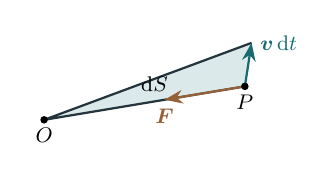
\begin{tikzpicture}[scale=0.85,transform shape]
\coordinate (O) at (0,0);\coordinate (P) at (3,.5);\coordinate (Q) at (3.1,1.15);
\fill[accent!15] (O)--(P)--(Q)--cycle;
\draw[object] (P)--(O)--(Q);
\draw[motion] (P)--(Q) node[right] {$\vect v\dd t$};
\draw[force] (P)--(1.8,.3) node[below] {$\vect F$};
\fill (O) circle (1.6pt) node[below] {$O$};\fill (P) circle (1.6pt) node[below] {$P$};
\node at (1.65,.54) {$\dd S$};
\end{tikzpicture}
\figcaption{变图4.1V1\quad 径向力的力矩为零，微小位移扫出以 $O$ 为顶点的面积。}
\end{minipage}\end{center}
\item 对圆轨道单独求周期。变图4.1V2 中，引力等于向心力，$mv^2/r=GMm/r^2$，故 $v^2=GM/r$。沿圆周一周的路程为 $2\pi r$，有 $T=2\pi r/v$，消去 $v$ 得 $T^2=4\pi^2r^3/(GM)$。椭圆的周期则由总面积 $\pi ab$ 除以面积速度求得，其半长轴 $a$ 进入最终公式。
\begin{center}\begin{minipage}{.98\linewidth}\centering
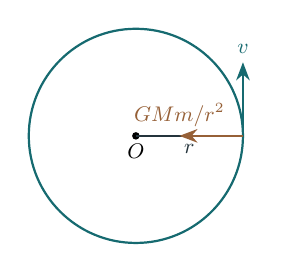
\begin{tikzpicture}[scale=0.85,transform shape]
\draw[traj] (0,0) circle (1.6);\fill (0,0) circle (1.6pt) node[below] {$O$};
\draw[object] (0,0)--(1.6,0) node[midway,below] {$r$};
\draw[motion] (1.6,0)--(1.6,1.1) node[above] {$v$};
\draw[force] (1.6,0)--(.65,0) node[above] {$GMm/r^2$};
\end{tikzpicture}
\figcaption{变图4.1V2\quad 圆轨道上，切向速度与固定半径一起确定周期。}
\end{minipage}\end{center}
\item 总能量为零时求轨道。取 $h\ne0$，将 $\varepsilon=0$ 代入离心率式得 $e^2=1$。于是变图4.1V3 的轨道为 $r=p/(1+\cos\varphi)$。在近点 $A$，$r=p/2$；当 $\varphi\to\pm\pi$，半径趋于无穷，轨道是一支抛物线。若 $h=0$，运动沿直线，能量式给 $|\dot r|=\sqrt{2\mu/r}$，方向由向内还是向外的初态决定。
\begin{center}\begin{minipage}{.98\linewidth}\centering
\begin{tikzpicture}[scale=0.85,transform shape]
\draw[axis] (-2.4,0)--(2.8,0) node[right] {$X$};
\draw[axis] (0,-2.6)--(0,2.6) node[above] {$Y$};
\draw[traj,domain=-110:110,samples=100] plot ({1.3*cos(\x)/(1+1*cos(\x))},{1.3*sin(\x)/(1+1*cos(\x))});
\fill (0,0) circle (1.7pt) node[below left] {$O$};
\fill ({1.3/(1+1)},0) circle (1.6pt) node[below right] {$A$};
\node[right] at (.9,1.7) {$\varepsilon=0,\ h\ne0$};
\end{tikzpicture}
\figcaption{变图4.1V3\quad 零能量、非零角动量给出焦点抛物线。}
\end{minipage}\end{center}
\item 改用 $\vect F=-k\vect r$。在变图4.1V4 中，力心为中心 $O=C$。两个坐标分别满足 $\ddot x+(k/m)x=0$、$\ddot y+(k/m)y=0$。将两坐标组合成同频简谐运动，得一般的中心椭圆，周期 $T=2\pi\sqrt{m/k}$ 与半长轴无关。角动量仍因零力矩保持，所以扫面积速度恒定。
\begin{center}\begin{minipage}{.98\linewidth}\centering
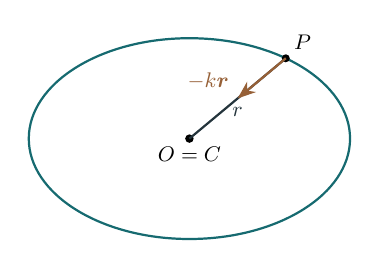
\begin{tikzpicture}[scale=0.85,transform shape]
\draw[traj] (0,0) ellipse (2.4 and 1.5);
\fill (0,0) circle (1.8pt) node[below] {$O=C$};
\coordinate (P) at (1.44,1.2);
\fill (P) circle (1.7pt) node[above right] {$P$};
\draw[object] (0,0)--(P) node[midway,below] {$r$};
\draw[force] (P)--(.72,.6) node[above left] {$-k\vect r$};
\end{tikzpicture}
\figcaption{变图4.1V4\quad 线性有心力的轨道以力心为椭圆中心。}
\end{minipage}\end{center}
\item 固定角动量，改变轨道能量。半通径 $p=h^2/\mu$ 保持，势阱最低值为 $-\mu^2/(2h^2)=-\mu/(2p)$，对应 $e=0$。变图4.1V5 以 $\mu/(2p)$ 为能量单位，画出 $e^2-1$ 所对应的各条水平线。由 $e^2=1+2\varepsilon h^2/\mu^2$，提高能量会依次得到椭圆、抛物线和双曲线。近点半径 $p/(1+e)$ 随之减小。负能量线与有效势的两个交点给出两拱点，零、正能量只保留有限的内转折点。
\begin{center}\begin{minipage}{.98\linewidth}\centering
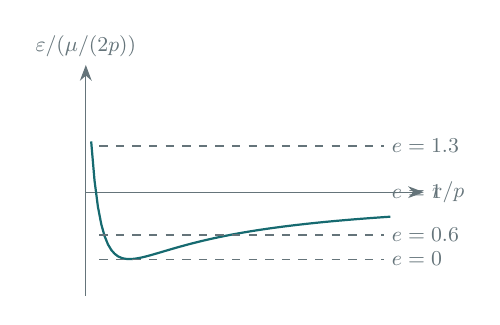
\begin{tikzpicture}[scale=0.85,transform shape]
\draw[axis] (.35,0)--(5.4,0) node[right] {$r/p$};
\draw[axis] (.35,-1.55)--(.35,1.9) node[above] {$\varepsilon/(\mu/(2p))$};
\draw[traj,domain=.43:4.9,samples=90] plot (\x,{2*(.5/\x^2-1/\x)});
\foreach \y/\txt in {-1/{e=0},-.64/{e=0.6},0/{e=1},.69/{e=1.3}}
 {\draw[guide] (.55,\y)--(4.8,\y) node[right] {$\txt$};}
\end{tikzpicture}
\figcaption{变图4.1V5\quad 固定半通径时，各能量水平线对应不同离心率。}
\end{minipage}\end{center}
\item 逐条给出三定律的计算依据。在变图4.1V6 上，以焦点 $O$ 为原点，由径向动力学与 $h=r^2\dot\varphi$ 得 $u''+u=\mu/h^2$，积分得到圆锥曲线。负能量筛选束缚椭圆，并以 $\varepsilon=-\mu/(2a)$ 确定半长轴。零力矩给面积速度 $h/2$。最后用 $r_Ar_B=b^2$ 求 $h=b\sqrt{\mu/a}$，再以 $\pi ab/(h/2)$ 得周期。
\begin{center}\begin{minipage}{.98\linewidth}\centering
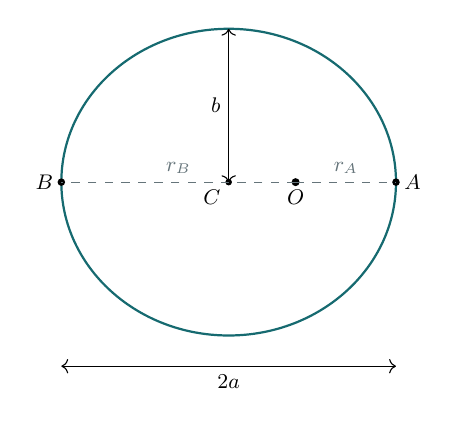
\begin{tikzpicture}[scale=0.85,transform shape]
\pgfmathsetmacro{\bb}{2.5*sqrt(1-0.4^2)}
\draw[traj] (0,0) ellipse (2.5 and \bb);
\coordinate (O) at ({2.5*0.4},0);\coordinate (C) at (0,0);
\fill (O) circle (1.7pt) node[below] {$O$};
\fill (C) circle (1.4pt) node[below left] {$C$};
\fill (2.5,0) circle (1.6pt) node[right] {$A$};
\fill (-2.5,0) circle (1.6pt) node[left] {$B$};
\draw[guide] (O)--(2.5,0) node[midway,above] {$r_A$};
\draw[guide] (O)--(-2.5,0) node[midway,above] {$r_B$};
\draw[<->] (-2.5,-2.75)--(2.5,-2.75) node[midway,below] {$2a$};
\draw[<->] (0,0)--(0,2.2913) node[midway,left] {$b$};
\end{tikzpicture}
\figcaption{变图4.1V6\quad 同一椭圆的两拱点与面积参数分别进入三条定律的推导。}
\end{minipage}\end{center}
\item 在万有引力之外增加向内加速度 $-kr$。总力仍沿径向，故面积定律保持。圆轨道满足 $r\omega^2=\mu/r^2+kr$，于是 $\omega^2=\mu/r^3+k$。变图4.1V7 将 $T=2\pi/\omega$ 写成 $T^2/r^3=4\pi^2/(\mu+kr^3)$，可见同一中心的该比值随 $r$ 改变。一般非圆轨道的方程多出与 $u^{-3}$ 成正比的项，通常形成进动轨道。
\begin{center}\begin{minipage}{.98\linewidth}\centering
\begin{tikzpicture}[scale=0.85,transform shape]
\draw[axis] (0,0)--(5.5,0) node[right] {$kr^3/\mu$};
\draw[axis] (0,0)--(0,3.4) node[above] {$\mu T^2/(4\pi^2r^3)$};
\draw[traj,domain=0:4.8,samples=65] plot (\x,{2.8/(1+\x)});
\node[left] at (0,2.8) {$1$};
\fill (1,1.4) circle (1.7pt) node[above right] {$(1,1/2)$};
\end{tikzpicture}
\figcaption{变图4.1V7\quad 额外线性引力使归一化周期常量随轨道半径改变。}
\end{minipage}\end{center}
\end{enumerate}

\clearpage

\pdfbookmark[2]{第 2 题 椭圆轨道反推平方反比引力}{q2}

\section*{第 2 题\quad 椭圆轨道反推平方反比引力}

\tagline{M-04-02}

已知行星沿椭圆轨道运动，太阳位于一个焦点，且径矢在相等时间内扫过相等面积。轨道的焦点极坐标方程为
\[
r=\frac{p}{1+e\cos\varphi},\qquad 0\leq e<1.
\]
试证明行星所受的力指向太阳，且大小与距离平方成反比。说明面积定律在证明中的作用，以及仅有轨道形状是否足够。

\par\medskip\noindent\begin{minipage}{\linewidth}\centering
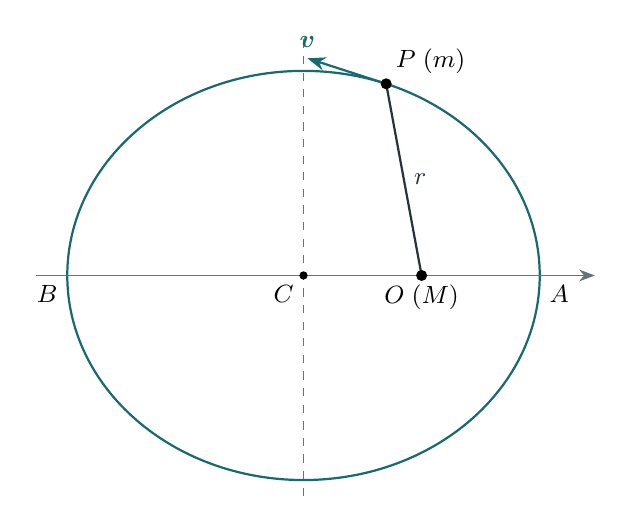
\begin{tikzpicture}[scale=1]
\draw[traj] (0.0000,0.0000) ellipse (3.0000 and 2.5981);

\coordinate (O) at (1.5,0);\coordinate (C) at (0,0);
\coordinate (P) at (1.05,2.434);\coordinate (A) at (3,0);\coordinate (B) at (-3,0);
\draw[axis] (-3.4,0)--(3.7,0);\draw[guide] (0,-2.8)--(0,3.0);
\draw[object] (O)--(P) node[midway,right] {$r$};
\draw[motion] (P)--++(-1.0,.324) node[above] {$\vect v$};
\fill (O) circle (2pt) node[below] {$O\;(M)$};\fill (C) circle (1.5pt) node[below left] {$C$};
\fill (P) circle (2pt) node[above right] {$P\;(m)$};
\node[below right] at (A) {$A$};\node[below left] at (B) {$B$};

\end{tikzpicture}
\figcaption{图 4.2　给定焦点椭圆及等面积时间规律。}
\end{minipage}\par\medskip

\Needspace{5\baselineskip}

\pdfbookmark[3]{题型定位}{q2-h0}

\subsection*{题型定位}

给定焦点椭圆及等面积时间规律，反求合力。由 $r(\varphi)$ 和 $r^2\dot\varphi=h$ 一起求两次时间导数，得出合力方向和随半径的变化。

\Needspace{5\baselineskip}

\pdfbookmark[3]{知识点}{q2-h1}

\subsection*{知识点}

\begin{itemize}
\tightlist
\item
  椭圆极坐标方程
\item
  极坐标径向加速度
\item
  角动量守恒
\item
  时间导数与角变量转换
\item
  平方反比力律反推
\end{itemize}

椭圆给出 $r(\varphi)$，面积定律给出角度随时间的变化。由恒定面积速度得到 $h=r^2\dot\varphi$，横向加速度为零。将它代入 Binet 公式，径向加速度随 $r$ 的平方反比变化。圆轨道的半径固定，只给出这个半径处的向心加速度。


\Needspace{5\baselineskip}

\pdfbookmark[3]{物理图像}{q2-h2}

\subsection*{物理图像}

行星沿以太阳为焦点的椭圆运动，径矢扫面积速度恒定。几何形状给出
\(r(\varphi)\)，面积定律再确定沿这条曲线的时间分配。

解图4.2A同时给出速度分量和转动的极坐标基矢，径向矢量加速度须取$\ddot r-r\dot\varphi^2$。解图4.2B则让同一椭圆按匀偏近点角运行，加速度转而指向椭圆中心，用于辨明轨道形状与运行时序的不同作用。

\Needspace{5\baselineskip}

\pdfbookmark[3]{解题入口}{q2-h3}

\subsection*{解题入口}

从椭圆方程 $r=p/(1+e\cos\varphi)$ 求 $\dot r=(eh/p)\sin\varphi$，再求 $\ddot r$。径向加速度还包含 $-r\dot\varphi^2$，两项合并得到 $-h^2/(pr^2)$。面积定律对时间求导则给横向加速度为零。

\Needspace{5\baselineskip}

\pdfbookmark[3]{标准解法}{q2-h4}

\subsection*{标准解法}

\subsubsection*{由面积定律确定时间参数}
令面积速度为 $\dot S=h/2$，其中 $h$ 为常量。于是
\[
r^2\dot\varphi=h,\qquad L=mh.
\]
求导得 $r\ddot\varphi+2\dot r\dot\varphi=0$，所以横向加速度为零，合力沿径向。还需计算径向加速度，才能判断其方向与距离依赖。

\par\medskip\noindent\begin{minipage}{\linewidth}\centering
\begin{tikzpicture}[scale=1]

\coordinate (O) at (0,0);\coordinate (P) at (3,1.6);
\draw[axis] (-.3,0)--(4.8,0) node[right] {极轴};
\draw[object] (O)--(P) node[midway,above] {$r$};
\draw[guide] (P)--(4.4,2.347);
\draw[motion] (P)--(3.9,2.08) node[above right] {$\dot r\,\vect e_r$};
\draw[motion] (3.9,2.08)--(3.33,3.15) node[right] {$r\dot\varphi\,\vect e_\varphi$};
\draw[motion] (P)--(3.33,3.15) node[left] {$\vect v$};
\draw[force] (P)--(1.9,1.013) node[below right] {$\vect F$};
\draw[muted] (.65,0) arc (0:28.072:.65) node[midway,right] {$\varphi$};
\fill (O) circle (2pt) node[below] {$O$};\fill (P) circle (2pt) node[below right] {$P$};

\end{tikzpicture}
\figcaption{解图 4.2A　径向加速度包含 $\ddot r$ 和 $-r\dot\varphi^2$ 两项。}
\end{minipage}\par\medskip

解图 4.2A 中，$\ddot r$ 表示径向坐标的二阶导数，$-r\dot\varphi^2$ 则来自基矢转动，两者相加才是 $a_r$。对轨道方程按时间求导：
\[
\dot r=\frac{pe\sin\varphi}{(1+e\cos\varphi)^2}\dot\varphi
=\frac{e\sin\varphi}{p}\,r^2\dot\varphi
=\frac{eh}{p}\sin\varphi.
\]
再求一次导数，得到
\[
\ddot r=\frac{eh}{p}\cos\varphi\,\dot\varphi
=\frac{eh^2}{pr^2}\cos\varphi.
\]
因此
\[
\begin{aligned}
a_r&=\ddot r-r\dot\varphi^2
=\frac{h^2}{r^2}\left(\frac{e\cos\varphi}p-\frac1r\right)\\
&=\frac{h^2}{r^2}\left[\frac{e\cos\varphi}p
 -\frac{1+e\cos\varphi}p\right]
=-\frac{h^2}{pr^2}.
\end{aligned}
\]
故
\[
\boxed{\vect F=-\frac{mh^2}{p}\frac1{r^2}\vect e_r
=-\frac{L^2}{mp}\frac1{r^2}\vect e_r}.
\]
负号表明力指向焦点，$mh^2/p$ 对此条轨道为常量。若把引力写作 $-GMm/r^2$，可识别 $GM=h^2/p$。

\subsubsection*{倒数半径与径向加速度}
令 $u=(1+e\cos\varphi)/p$，则 $u''+u=1/p$。由 $\dot r=-hu'$ 可得
\[
a_r=-h^2u^2(u''+u)=-\frac{h^2}{pr^2},
\]
与直接求导相同。

椭圆给出 $r$ 随极角的关系，面积定律再给出极角随时间的变化。两条条件合在一起，使 $r^2\dot\varphi$ 为常量，力沿径向且随半径的平方反比变化。$e=0$ 时半径固定，运动方程给出该半径处的向心力值。
\subsubsection*{偏近点角匀速时的受力与面积速度}
取非圆椭圆$0<e<1$，令焦点仍为$O$，以恒定角速率$\Omega$改变偏近点角，
人为规定
\[
X=a(\cos\Omega t-e),\qquad Y=b\sin\Omega t.
\]
这一运动沿同一条几何椭圆，时间参数改为匀速的偏近点角。对两坐标分别求两次时间导数，得到
\[
\ddot X=-\Omega^2(X+ae),\qquad
\ddot Y=-\Omega^2Y.
\]
因此合力指向椭圆中心$C=(-ae,0)$，为
$\vect F=-m\Omega^2(\vect r-\vect r_C)$，一般不指向焦点$O$。
解图4.2B 标出同一个轨道点指向 $C$ 和指向 $O$ 的方向。沿同一条椭圆改变运动的时间分配，便得到指向不同点的力。
\begin{center}\begin{minipage}{\linewidth}\centering
\begin{tikzpicture}[scale=.8]
\draw[traj](0,0)ellipse(3 and 2.598076);
\fill(0,0)circle(2pt);\node[below]at(0,0){$C$};
\fill(1.5,0)circle(2pt);\node[below]at(1.5,0){$O$};
\fill(1.05,2.43375)circle(2pt);\node[above]at(1.05,2.43375){$P$};
\draw[guide](1.05,2.43375)--(0,0);\draw[guide](1.05,2.43375)--(1.5,0);
\draw[force](1.05,2.43375)--(.525,1.216875)node[left]{$\vect F_C$};
\node[align=left,anchor=west]at(3.6,1.4){恒定偏近点角速率\\力指向中心$C$\\不满足对$O$的面积定律};
\end{tikzpicture}
\figcaption{解图4.2B\quad 相同几何椭圆、不同时间分配可以对应不同的力。}
\end{minipage}\end{center}
对这个反例，直接求焦点面积速度也得
\[
X\dot Y-Y\dot X=ab\Omega(1-e\cos\Omega t),
\]
因此在这种时间分配下，焦点面积速度随时间改变。题设的面积定律使 $r^2\dot\varphi$ 恒定，对应前面指向焦点的力。该轨道给出的力常量为 $mh^2/p$。若比较多颗行星，则由各自的 $h^2/p$ 或周期数据判断它们是否对应同一个 $GM$。非圆椭圆的半径在近、远点之间连续变化，平方反比关系在这一段半径范围内得到。单条圆轨道则给出固定半径处的一个向心力值。


\Needspace{5\baselineskip}

\pdfbookmark[3]{关键洞察}{q2-h5}

\subsection*{关键洞察}

焦点椭圆给出 $r(\varphi)$，面积定律把每一点的角速度定为 $h/r^2$。两次链式求导都使用这个角速度，所得径向加速度才包含随距离变化的确切系数。

解图4.2B 让非圆椭圆的偏近点角匀速变化，得到指向中心 $C$ 的力，焦点 $O$ 的面积速度随时间改变。按题设面积定律运动时，力指向焦点。圆形极限中两点重合，受力值对应单一半径。

\Needspace{5\baselineskip}

\pdfbookmark[3]{易错点}{q2-h6}

\subsection*{易错点}

\begin{itemize}
\item 径向矢量加速度为 $\ddot r-r\dot\varphi^2$，后一项来自基矢转动。
\item 对 $r(\varphi)$ 求时间导数时，乘上 $\dot\varphi$，第二次求导继续使用链式法则。
\item 面积定律给 $r^2\dot\varphi=h$，用它消去时间导数中的角速度。
\item 横向加速度为零给出有心方向，径向计算的 $-h^2/(pr^2)$ 给出力的大小和符号。
\item 参数 $p,e$ 描述轨道几何，$mh^2/p$ 是反推出的力系数。
\item 椭圆的几何形状和面积随时间的规律一起确定合加速度。
\end{itemize}

\Needspace{5\baselineskip}

\pdfbookmark[3]{课堂讲解建议}{q2-h7}

\subsection*{课堂讲解建议}

在解图4.2A 先用面积定律求 $h$，逐次写出两次链式求导。问为什么 $\ddot r$ 还要减去 $r\dot\varphi^2$，由径向基矢随角度转动解释。再看解图4.2B，问同一椭圆按匀偏近点角运动时力指向哪里，答案是中心 $C$，焦点面积速度随之改变。最后用变图4.2V1 说明单个圆轨道给一个半径处的力值，一族周期数据才给距离函数。

\Needspace{5\baselineskip}

\pdfbookmark[3]{变式训练}{q2-h8}

\subsection*{变式训练}

\begin{enumerate}
\item 由一族圆轨道的周期反推力律。变图4.2V1 中，给定一条圆的半径 $r$ 和周期 $T$，速度为 $2\pi r/T$，径向力大小为 $4\pi^2mr/T^2$。若不同半径的圆都满足 $T^2/r^3=C$，代入得 $F=4\pi^2m/(Cr^2)$。因此单条圆给一个力值，一族相同常量的周期数据给出距离的平方反比关系。
\begin{center}\begin{minipage}{.98\linewidth}\centering
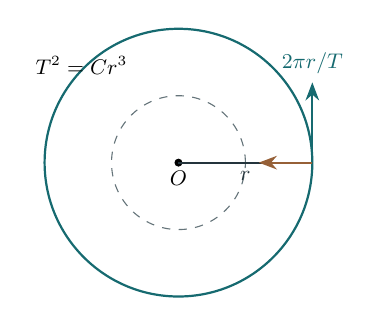
\begin{tikzpicture}[scale=0.85,transform shape]
\draw[guide] (0,0) circle (1);\draw[traj] (0,0) circle (2);
\fill (0,0) circle (1.7pt) node[below] {$O$};
\draw[object] (0,0)--(2,0) node[midway,below] {$r$};
\draw[motion] (2,0)--(2,1.2) node[above] {$2\pi r/T$};
\draw[force] (2,0)--(1.2,0);
\node at (-1.45,1.45) {$T^2=Cr^3$};
\end{tikzpicture}
\figcaption{变图4.2V1\quad 一族不同半径的圆轨道由周期数据给出速度和向心加速度。}
\end{minipage}\end{center}
\item 若焦点扫面积速度随时间改变，求横向力。由 $L=2m\dot S$，有 $\dot L=2m\ddot S$。变图4.2V2 中，径向力对 $O$ 的力矩为零，横向力的力矩为 $rF_\varphi$，所以 $F_\varphi=2m\ddot S/r$。扫面积速度正在改变的时刻具有非零横向合力；仅有椭圆形状还缺少时间规律。
\begin{center}\begin{minipage}{.98\linewidth}\centering
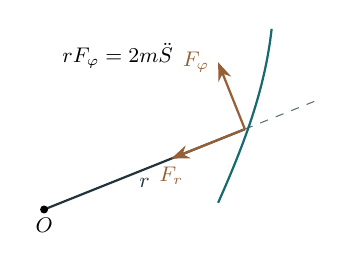
\begin{tikzpicture}[scale=0.85,transform shape]
\coordinate (O) at (0,0);\coordinate (P) at (3,1.2);
\draw[object] (O)--(P) node[midway,below] {$r$};
\draw[force] (P)--(1.9,.76) node[below] {$F_r$};
\draw[force] (P)--(2.6,2.2) node[left] {$F_\varphi$};
\draw[guide] (P)--(4.1,1.64);
\fill (O) circle (1.7pt) node[below] {$O$};
\draw[traj] (2.6,.1) .. controls (3.0,1.0) and (3.3,1.8) .. (3.4,2.7);
\node at (1.1,2.3) {$rF_\varphi=2m\ddot S$};
\end{tikzpicture}
\figcaption{变图4.2V2\quad 扫面积速度改变时，横向力与关于 $O$ 的力矩对应。}
\end{minipage}\end{center}
\item 给定抛物线及面积定律，反求力。变图4.2V3 的焦点极坐标为 $u=(1+\cos\varphi)/p$，故 $u'=-\sin\varphi/p$、$u''=-\cos\varphi/p$，两项相加为 $u''+u=1/p$。恒定 $h=r^2\dot\varphi$ 给 $a_r=-h^2u^2(u''+u)$，所以 $F_r=-mh^2/(pr^2)$。同一反推也适用于抛物线，角动量取非零值。
\begin{center}\begin{minipage}{.98\linewidth}\centering
\begin{tikzpicture}[scale=0.85,transform shape]
\draw[axis] (-2.4,0)--(2.8,0) node[right] {$X$};
\draw[axis] (0,-2.6)--(0,2.6) node[above] {$Y$};
\draw[traj,domain=-110:110,samples=100] plot ({1.3*cos(\x)/(1+1*cos(\x))},{1.3*sin(\x)/(1+1*cos(\x))});
\fill (0,0) circle (1.7pt) node[below left] {$O$};
\fill ({1.3/(1+1)},0) circle (1.6pt) node[below right] {$A$};
\node[right] at (1.35,1.6) {$u''+u=1/p$};
\end{tikzpicture}
\figcaption{变图4.2V3\quad 同一倒数半径方程也适用于抛物线。}
\end{minipage}\end{center}
\item 用倒数半径重新求径向加速度。变图4.2V4 画出 $pu=1+e\cos\varphi$，其二阶角导数为 $pu''=-e\cos\varphi$，相加只留下 $1$。由链式法则 $\dot r=-hu'$、$\ddot r=-h^2u^2u''$，另有 $r\dot\varphi^2=h^2u^3$。因此 $a_r=\ddot r-r\dot\varphi^2=-h^2u^2(u''+u)=-h^2/(pr^2)$。
\begin{center}\begin{minipage}{.98\linewidth}\centering
\begin{tikzpicture}[scale=0.85,transform shape]
\draw[axis] (0,0)--(6.3,0) node[right] {$\varphi$};
\draw[axis] (0,0)--(0,3) node[above] {$pu$};
\draw[traj,domain=0:360,samples=85] plot ({\x/62},{1.65*(1+.5*cos(\x))});
\draw[guide] (0,1.65)--(5.85,1.65);
\node[left] at (0,1.65) {$1$};
\node[left] at (0,2.475) {$1+e$};
\node[below] at ({180/62},0) {$\pi$};
\node[below] at ({360/62},0) {$2\pi$};
\end{tikzpicture}
\figcaption{变图4.2V4\quad 倒数半径由常数项与余弦项组成，两次角导数使余弦项相消。}
\end{minipage}\end{center}
\item 取偏心率趋于零的极限。轨道成为变图4.2V5 中半径为 $p$ 的圆，$\dot r=0$、$\dot\varphi=h/p^2$。圆速为 $p\dot\varphi=h/p$，所以 $a_r=-(h/p)^2/p=-h^2/p^3$，正好是通式在 $r=p$ 的值。圆的运动只经过一个半径，力在其他半径的函数形式还需其他运动数据确定。
\begin{center}\begin{minipage}{.98\linewidth}\centering
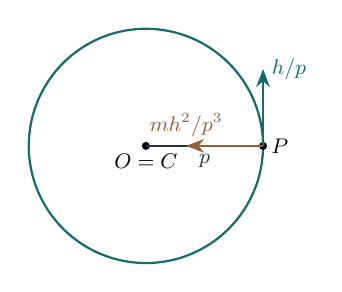
\begin{tikzpicture}[scale=0.85,transform shape]
\draw[traj] (0,0) circle (1.75);
\fill (0,0) circle (1.7pt) node[below] {$O=C$};
\fill (1.75,0) circle (1.7pt) node[right] {$P$};
\draw[object] (0,0)--(1.75,0) node[midway,below] {$p$};
\draw[motion] (1.75,0)--(1.75,1.15) node[right] {$h/p$};
\draw[force] (1.75,0)--(.6,0) node[above] {$mh^2/p^3$};
\end{tikzpicture}
\figcaption{变图4.2V5\quad 圆极限的半径固定，匀角速度给出此半径处的向心加速度。}
\end{minipage}\end{center}
\item 令球沿同一非圆椭圆以恒定速率运动。变图4.2V6 中，加速度沿曲线法线，焦点到切线的垂距记为 $d$，角动量大小为 $L=mvd$。在长轴两端，切线都垂直长轴。近、远点的速度均垂直焦点径矢，恒定速率使两处 $L$ 分别为 $mv a(1-e)$ 与 $mv a(1+e)$。因此 $e>0$ 时角动量改变，过程中存在横向力。圆的 $e=0$ 情形则有恒定角动量。
\begin{center}\begin{minipage}{.98\linewidth}\centering
\begin{tikzpicture}[scale=0.85,transform shape]
\pgfmathsetmacro{\bb}{2.5*sqrt(1-0.6^2)}
\draw[traj] (0,0) ellipse (2.5 and \bb);
\coordinate (O) at ({2.5*0.6},0);\coordinate (C) at (0,0);
\fill (O) circle (1.7pt) node[below] {$O$};
\fill (C) circle (1.4pt) node[below left] {$C$};
\fill (2.5,0) circle (1.6pt) node[right] {$A$};
\fill (-2.5,0) circle (1.6pt) node[left] {$B$};
\coordinate (P) at ({2.5*cos(60)},{2*sin(60)});
\draw[guide] (O)--(2.115384615,1.332346775) node[midway,right] {$d$};
\fill (2.115384615,1.332346775) circle (1.3pt);
\draw[object] (P)++({-1.3*sin(60)},{1.04*cos(60)})--++({2.6*sin(60)},{-2.08*cos(60)});
\draw[force] (P)--++({-.4*cos(60)},{-.5*sin(60)}) node[below left] {$\vect F$};
\node[right] at (2.7,.8) {$v=\text{常量}$};
\end{tikzpicture}
\figcaption{变图4.2V6\quad 恒速沿非圆椭圆运动时，加速度沿曲线法线。}
\end{minipage}\end{center}
\item 说明面积定律在反推中的两次作用。变图4.2V7 的微元给 $r^2\dot\varphi=h$。第一次把它用于对轨道求时间导数，使 $\dot r=(eh/p)\sin\varphi$，再求导后与基矢转动项合并得到径向加速度。第二次对 $r^2\dot\varphi=h$ 求导，得 $r\ddot\varphi+2\dot r\dot\varphi=0$，令横向加速度为零。两项合起来给出完整的加速度向量。
\begin{center}\begin{minipage}{.98\linewidth}\centering
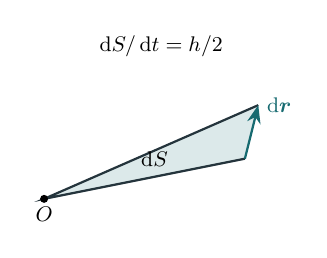
\begin{tikzpicture}[scale=0.85,transform shape]
\coordinate (O) at (0,0);\coordinate (P) at (3,.6);\coordinate (Q) at (3.2,1.4);
\fill[accent!15] (O)--(P)--(Q)--cycle;
\draw[object] (P)--(O)--(Q);
\draw[motion] (P)--(Q) node[right] {$\dd\vect r$};
\fill (O) circle (1.7pt) node[below] {$O$};
\node at (1.65,.6) {$\dd S$};
\node[above] at (1.75,2) {$\dd S/\dd t=h/2$};
\end{tikzpicture}
\figcaption{变图4.2V7\quad 同一面积微元既给角速度，也给横向加速度的约束。}
\end{minipage}\end{center}
\end{enumerate}

\clearpage

\pdfbookmark[2]{第 3 题 初速度决定有心轨道类型}{q3}

\section*{第 3 题\quad 初速度决定有心轨道类型}

\tagline{M-04-03}

质量为 $M$ 的恒星固定不动，质量为 $m$ 的行星仅受其引力。行星位于距离 $r_0$ 处，初速 $v_0>0$ 与径矢垂直。讨论轨道为椭圆、圆、抛物线、双曲线时 $v_0$ 的取值，并指出椭圆情形下初始点是近点还是远点。另说明 $v_0=0$ 的退化情形。

\par\medskip\noindent\begin{minipage}{\linewidth}\centering
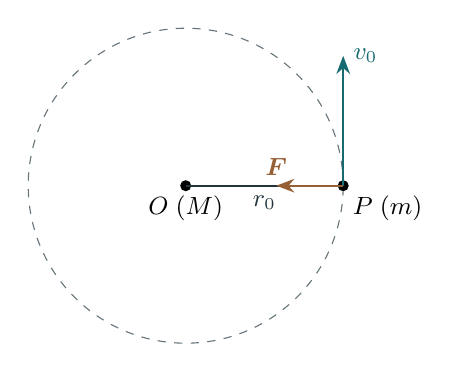
\begin{tikzpicture}[scale=1]

\draw[guide] (0,0) circle (2);\fill (0,0) circle (2pt) node[below] {$O\;(M)$};
\fill (2,0) circle (2pt) node[below right] {$P\;(m)$};
\draw[object] (0,0)--(2,0) node[midway,below] {$r_0$};
\draw[motion] (2,0)--(2,1.65) node[right] {$v_0$};
\draw[force] (2,0)--(1.15,0) node[above] {$\vect F$};

\end{tikzpicture}
\figcaption{图 4.3　初速度垂直于径矢；虚线圆用于比较轨道。}
\end{minipage}\par\medskip

\Needspace{5\baselineskip}

\pdfbookmark[3]{题型定位}{q3-h0}

\subsection*{题型定位}

切向初速度决定轨道类型的判别题。初始距离给定，\(r_0v_0\)
确定比角动量，初始能量符号决定束缚或逃逸；圆轨道还要求切向速率恰等于当地圆速。

题目需同时区分圆速与逃逸速、圆与非圆椭圆、近点与远点。由于初速垂直径矢，初始点是拱点；若取消这个方向条件，能量分类仍成立，但圆轨道与拱点判断需要重做。

\Needspace{5\baselineskip}

\pdfbookmark[3]{知识点}{q3-h1}

\subsection*{知识点}

\begin{itemize}
\tightlist
\item
  总机械能判别轨道类型
\item
  逃逸速度
\item
  圆轨道速度
\item
  切向初速度与角动量
\item
  椭圆、抛物线、双曲线分类
\end{itemize}

轨道分类先看比机械能及非零角动量，离心率由两者组合确定。切向初速相对当地圆速决定初始点是近点、远点还是圆轨道，逃逸边界由零能量给出。零角动量时运动沿径向直线。非退化抛物线则同时满足比能量为零与角动量非零。


\Needspace{5\baselineskip}

\pdfbookmark[3]{物理图像}{q3-h2}

\subsection*{物理图像}

图4.3的初速度沿切向，初始点的径向速度为零。当地圆速$v_c$使引力恰好维持固定半径；低于圆速时初点是椭圆远点，高于圆速但未达到逃逸速时是椭圆近点。圆速 $v_c$ 对应固定半径，逃逸速 $v_e=\sqrt2v_c$ 对应零比能量，它们在速率轴上标出两个不同位置。

图中真实引力矢量始终向$O$，而半径坐标的$\ddot r$还含切向运动的几何项。解图4.3A把速度轴分成低于圆速、圆速、圆速到逃逸速度及非束缚区间；短时间直角坐标展开解释半径为何可在向内引力下增大。零初速径向坠落须单列，不套用非零角动量的圆锥曲线分类。

\Needspace{5\baselineskip}

\pdfbookmark[3]{解题入口}{q3-h3}

\subsection*{解题入口}

先由比能量 $v_0^2/2-\mu/r_0$ 的符号区分束缚、零能逃逸和正能逃逸。圆速由引力等于向心需求给出。在纯切向初速下，令 $q=v_0^2/v_c^2$，用另一拱点半径 $qr_0/(2-q)$ 与 $r_0$ 比较，确定初态是近点还是远点。

\Needspace{5\baselineskip}

\pdfbookmark[3]{标准解法}{q3-h4}

\subsection*{标准解法}

\subsubsection*{能量决定束缚与逃逸}
记 $\mu=GM$。初态的比能量与比角动量为
\[
\varepsilon=\frac12v_0^2-\frac\mu{r_0},\qquad h=r_0v_0.
\]
令 $\varepsilon=0$，得到逃逸速度
\[
v_e=\sqrt{\frac{2\mu}{r_0}}.
\]
$v_0=v_e$ 时为抛物线，速率在无穷远处趋零；$v_0>v_e$ 时为双曲线，远处仍有 $v_\infty=\sqrt{v_0^2-v_e^2}>0$；$0<v_0<v_e$ 时为束缚椭圆，圆轨道包括在内。

\subsubsection*{圆轨道与初始拱点}
圆轨道要求引力提供向心加速度：
\[
\frac\mu{r_0^2}=\frac{v_c^2}{r_0},\qquad
v_c=\sqrt{\frac\mu{r_0}}=\frac{v_e}{\sqrt2}.
\]
从椭圆能量也可得到同一结果。若近、远点半径为 $r_A,r_B$，能量与角动量联立给出
\[
\frac1{r_A}+\frac1{r_B}=\frac{2\mu}{h^2},\qquad
\frac1{r_Ar_B}=-\frac{2\varepsilon}{h^2}.
\]
两式相除，使用 $r_A+r_B=2a$，得
\[
2a=-\frac\mu\varepsilon,\qquad
\frac1a=\frac2{r_0}-\frac{v_0^2}\mu.
\]
圆轨道取 $a=r_0$，仍得 $v_c^2=\mu/r_0$。在这一区间中，负能量给出束缚轨道。再取初速纯切向且 $v_0=v_c$，半径保持为 $r_0$，才得到圆。

\par\medskip\noindent\begin{minipage}{\linewidth}\centering
\begin{tikzpicture}[scale=0.94]

\draw[axis] (0,0)--(10,0) node[right] {$v_0$};
\foreach \x/\lab in {0/0,4/{v_c},5.656854/{v_e=\sqrt2v_c}} {\draw[ink] (\x,-.12)--(\x,.12);\node[below] at (\x,-.12) {$\lab$};}
\node[above,align=center] at (2,.4) {椭圆\\$P$ 为远点};
\node[above,align=center] at (4.828427,.4) {椭圆\\$P$ 为近点};
\node[above] at (4,1.8) {圆};\draw[guide] (4,.2)--(4,1.7);
\node[above] at (5.656854,1.8) {抛物线};\draw[guide] (5.656854,.2)--(5.656854,1.7);
\node[above] at (8.7,.4) {双曲线};
\node[below] at (2,-.9) {$E<0$};\node[below] at (8.7,-.9) {$E>0$};

\end{tikzpicture}
\figcaption{解图 4.3A　圆轨道速度与逃逸速度给出两个不同的分类界限。}
\end{minipage}\par\medskip

初速为纯切向，所以 $\dot r(0)=0$。径向方程给出
\[
\ddot r(0)=\frac{v_0^2-v_c^2}{r_0}.
\]
若 $v_0<v_c$，半径随后减小，初始点 $P$ 是远点；若 $v_c<v_0<v_e$，半径随后增加，$P$ 是近点。解图 4.3A 因而把椭圆区间分成两段。完整分类为
\[
\begin{array}{c|c|c}
\text{初速}&\text{轨道}&\text{初始点}\\\hline
0<v_0<v_c&\text{非圆椭圆}&\text{远点}\\
v_0=v_c&\text{圆}&\text{任一点}\\
v_c<v_0<v_e&\text{非圆椭圆}&\text{近点}\\
v_0=v_e&\text{抛物线}&\text{近点}\\
v_0>v_e&\text{双曲线}&\text{近点}
\end{array}
\]
设 $s=v_0/v_c$，把初速代入比能量与角动量，离心率可写为
\[
e^2=1+\frac{2\varepsilon h^2}{\mu^2}
=1+(s^2-2)s^2=(s^2-1)^2.
\]
即 $e=|s^2-1|$。若 $v_0=0$，角动量 $h=0$，比能量为 $-\mu/r_0$，行星沿径向坠落。这是 $e=1$ 的退化直线轨道。非退化抛物线对应 $e=1$ 且比能量为零。
\subsubsection*{同一初始点对应的另一拱点}
令$q=v_0^2/v_c^2$，则$h^2=q\mu r_0$，$\varepsilon=(q/2-1)\mu/r_0$。
对$0<q<2$，半长轴、离心率和半通径分别为
\[
a=\frac{r_0}{2-q},\qquad e=|q-1|,\qquad p=qr_0.
\]
初始点本就是一个拱点，另一拱点的半径可由两者之和$2a$求得：
\[
r_{\rm other}=2a-r_0=\frac{q}{2-q}r_0,
\qquad v_{\rm other}=\frac{r_0}{r_{\rm other}}v_0
=\frac{2-q}{q}v_0.
\]
解图4.3A 的两个非圆椭圆区间以 $q=1$ 分开。$0<q<1$ 时，另一拱点比 $r_0$ 更靠近恒星，初态是远点；$1<q<2$ 时，另一拱点离恒星更远，初态是近点。用同一式比较 $r_{\rm other}$ 与 $r_0$，也就确定了初态径向距离随后是减小还是增大。
当$q\to2^-$，远点与半长轴都趋于无穷，而近点仍为$r_0$，
椭圆连续趋向以初始点为近点的抛物线。

\subsubsection*{引力向内，为什么半径还可能增大}
图4.3的引力箭头始终指向$O$，它给出的初始矢量加速度是
$-\mu\vect e_r/r_0^2$，与$v_0$是否超过圆速无关。
半径坐标的二阶导数却为
\[
\ddot r(0)=-\frac\mu{r_0^2}+r_0\dot\varphi(0)^2
=\frac{v_0^2}{r_0}-\frac\mu{r_0^2}.
\]
正的 $r_0\dot\varphi(0)^2$ 项来自切向位移对半径的几何贡献。真实的矢量加速度仍只有向内的引力加速度。
在初始点附近取直角坐标，$P=(r_0,0)$，初速度沿正$y$，则
\[
x(t)=r_0-\frac{\mu}{2r_0^2}t^2+O(t^3),\qquad
y(t)=v_0t+O(t^3),
\]
\[
r(t)=r_0+\frac12\left(\frac{v_0^2}{r_0}-\frac\mu{r_0^2}\right)t^2+O(t^3).
\]
因此尽管$x$坐标正在向恒星一侧弯曲，足够大的切向位移仍可使总距离$r$增大。
这就是近点之后向外运动与引力始终向内能够同时成立的原因。
比较 $v_0^2/r_0$ 与 $\mu/r_0^2$ 就能确定半径的初始变化。二者相等且初速纯切向时，向心加速度与保持该圆所需的值一致。

若进一步给恒星半径$R<r_0$，低于圆速的形式椭圆还可能穿过星体。
其近点为$r_{min}=qr_0/(2-q)$，要避免接触须
\[
q>\frac{2R}{r_0+R},\qquad
v_0>v_c\sqrt{\frac{2R}{r_0+R}}.
\]
等号对应轨道与表面相切。题设的理想点引力中心对应半径取零。


\Needspace{5\baselineskip}

\pdfbookmark[3]{关键洞察}{q3-h5}

\subsection*{关键洞察}

能量符号决定能否逃逸，圆轨道还需要速率和方向同时满足条件。初速纯切向时，\(\ddot r(0)\)
的符号直接说明初始点是近点还是远点。

解图4.3A中两个椭圆区间由 \(v_c\) 分开，\(v_e\)
才是逃逸边界。零初速使角动量为零，后续是直线坠落。普通抛物线具有非零角动量和零能量。

\Needspace{5\baselineskip}

\pdfbookmark[3]{易错点}{q3-h6}

\subsection*{易错点}

\begin{itemize}
\item 圆速 $v_c=\sqrt{\mu/r_0}$ 保持半径，逃逸速 $v_e=\sqrt{2\mu/r_0}$ 使比能量为零。
\item 圆的初速度沿切线且大小为 $v_c$。
\item 纯切向初速给 $\dot r(0)=0$，再以 $\ddot r(0)$ 的正负确定近点或远点。
\item 势能以无穷远为零，写成 $-\mu m/r$。动能取完整速率平方。
\item $0<v_0<v_c$ 与 $v_c<v_0<v_e$ 都是非圆椭圆，$v_0=v_c$ 时为圆。
\end{itemize}

\Needspace{5\baselineskip}

\pdfbookmark[3]{课堂讲解建议}{q3-h7}

\subsection*{课堂讲解建议}

在解图4.3A 的横轴上先标圆速 $v_c$ 和逃逸速 $\sqrt2v_c$，请学生分别给出两处的径向加速度和能量。接着对照变图4.3V1 与V2，在两张椭圆上找到相同的初始距离 $r_0$，说明另一拱点为何一内一外。再看变图4.3V3，把初速度分为径向与横向，问初点是否仍是拱点，由 $\dot r(0)$ 的值回答。

\Needspace{5\baselineskip}

\pdfbookmark[3]{变式训练}{q3-h8}

\subsection*{变式训练}

\begin{enumerate}
\item 取 $v_0=v_c/2$。此时 $q=1/4$，故 $e=|q-1|=3/4$，$a=r_0/(2-q)=4r_0/7$。变图4.3V1 中 $P$ 是远点，另一拱点 $A$ 的半径为 $2a-r_0=r_0/7$。也可取 $p=qr_0=r_0/4$，代入 $p/(1+e)$ 得同一近点。由角动量，近点速率为 $r_0v_0/(r_0/7)=7v_c/2$。
\begin{center}\begin{minipage}{.98\linewidth}\centering
\begin{tikzpicture}[scale=0.85,transform shape]
\draw[axis] (-0.8571428571428572,0)--(3.8000000000000003,0);
\draw[traj] (1.3714285714285714,0) ellipse ({1.8285714285714285} and {1.8285714285714285*sqrt(1-0.75^2)});
\fill (0,0) circle (1.7pt) node[below] {$O$};
\fill (3.2,0) circle (1.7pt) node[right] {$P$};
\draw[object] (0,0)--(3.2,0) node[midway,below] {$r_0$};
\draw[motion] (3.2,0)--(3.2,.9) node[right] {$v_c/2$};
\fill ({-3.2/7},0) circle (1.7pt) node[left] {$A$};
\node at (1.15,1.45) {$P$ 是远点};
\end{tikzpicture}
\figcaption{变图4.3V1\quad 低于圆速的切向初速使初始点成为远点，另一拱点距恒星更近。}
\end{minipage}\end{center}
\item 取 $v_0=1.2v_c$。$q=1.44$ 介于 $1$ 和 $2$ 之间，故比能量为负，而初始半径的二阶导数为正，$P$ 是近点。变图4.3V2 的半长轴 $a=25r_0/14$，离心率 $e=.44$，远点半径 $r_B=2a-r_0=18r_0/7$。远点速率由 $r_Bv_B=r_0v_0$ 给出 $v_B=7v_c/15$。
\begin{center}\begin{minipage}{.98\linewidth}\centering
\begin{tikzpicture}[scale=0.85,transform shape]
\draw[axis] (-4.257142857142858,0)--(2.1,0);
\draw[traj] (-1.1785714285714286,0) ellipse ({2.678571428571429} and {2.678571428571429*sqrt(1-0.44^2)});
\fill (0,0) circle (1.7pt) node[below] {$O$};
\fill (1.5,0) circle (1.7pt) node[right] {$P$};
\draw[object] (0,0)--(1.5,0) node[midway,below] {$r_0$};
\draw[motion] (1.5,0)--(1.5,1.4) node[right] {$1.2v_c$};
\fill ({-27/7},0) circle (1.7pt) node[left] {$B$};
\node at (-1.35,1.95) {$P$ 是近点};
\end{tikzpicture}
\figcaption{变图4.3V2\quad 高于圆速而低于逃逸速，初点变为近点。}
\end{minipage}\end{center}
\item 若初速含径向分量，怎样确定轨道？变图4.3V3 给 $v_0^2=v_{r0}^2+v_{\varphi0}^2$，所以比能量仍是 $v_0^2/2-\mu/r_0$。比角动量大小为 $h=r_0|v_{\varphi0}|$。当 $h>0$ 时，将它代入 $e^2=1+2\varepsilon h^2/\mu^2$，按比能量的符号分类。若 $v_{r0}\ne0$，初点的半径正在改变。椭圆上它位于两个拱点之间，抛物线或双曲线上它位于唯一的近点之外。圆轨道的初态同时满足 $v_{r0}=0$、$|v_{\varphi0}|=v_c$。若 $h=0$，初速度沿径向，由径向能量方程确定行进过程。
\begin{center}\begin{minipage}{.98\linewidth}\centering
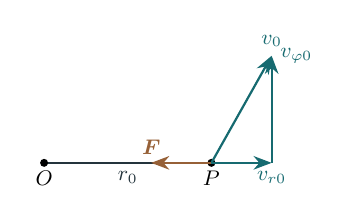
\begin{tikzpicture}[scale=0.85,transform shape]
\coordinate (O) at (0,0);\coordinate (P) at (2.5,0);
\draw[object] (O)--(P) node[midway,below] {$r_0$};
\fill (O) circle (1.7pt) node[below] {$O$};\fill (P) circle (1.7pt) node[below] {$P$};
\draw[motion] (P)--(3.4,0) node[below] {$v_{r0}$};
\draw[motion] (3.4,0)--(3.4,1.6) node[right] {$v_{\varphi0}$};
\draw[motion] (P)--(3.4,1.6) node[above] {$v_0$};
\draw[force] (P)--(1.6,0) node[above] {$\vect F$};
\end{tikzpicture}
\figcaption{变图4.3V3\quad 斜向初速度中，两分量都贡献能量，只有横向分量贡献角动量。}
\end{minipage}\end{center}
\item 用逃逸速度求恒星质量。将无穷远势能定为零，边缘逃逸的比能量为零，故 $v_e^2/2-GM/r_0=0$，得 $M=v_e^2r_0/(2G)$。变图4.3V4 中，测得一组 $(r_0,v_e^2)$ 就给出曲线上的一点，乘积 $r_0v_e^2$ 为 $2GM$。这里的逃逸速度指只受该恒星引力、向无穷远运动时速度趋零的条件。
\begin{center}\begin{minipage}{.98\linewidth}\centering
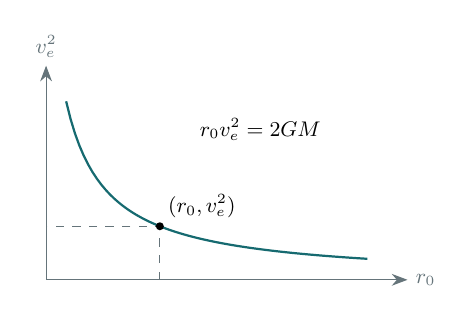
\begin{tikzpicture}[scale=0.85,transform shape]
\draw[axis] (.3,0)--(5.7,0) node[right] {$r_0$};
\draw[axis] (.3,0)--(.3,3.2) node[above] {$v_e^2$};
\draw[traj,domain=.6:5.1,samples=70] plot (\x,{1.6/\x});
\draw[guide] (2,0)--(2,.8)--(.3,.8);
\fill (2,.8) circle (1.7pt) node[above right] {$(r_0,v_e^2)$};
\node at (3.5,2.25) {$r_0v_e^2=2GM$};
\end{tikzpicture}
\figcaption{变图4.3V4\quad 逃逸速度平方与测量距离的乘积给出恒星质量。}
\end{minipage}\end{center}
\item 比较同一半径圆轨道与抛物线的能量。圆轨道动能为 $\mu m/(2r_0)$、势能为 $-\mu m/r_0$，总能量 $E_c=-\mu m/(2r_0)$。抛物线总能量 $E_p=0$，因此切向加速需增加机械能 $\mu m/(2r_0)$。变图4.3V5 的长速度箭头由圆速和脉冲增量组成，$\Delta v=v_e-v_c=(\sqrt2-1)v_c$。两状态在同一点具有相同势能，所增机械能都表现为动能增加。
\begin{center}\begin{minipage}{.98\linewidth}\centering
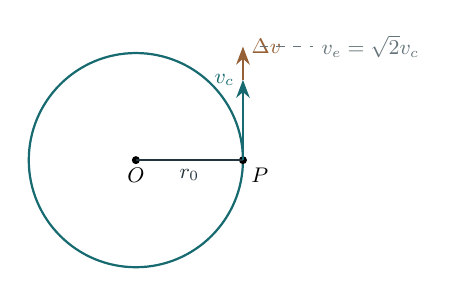
\begin{tikzpicture}[scale=0.85,transform shape]
\draw[traj] (0,0) circle (1.6);
\fill (0,0) circle (1.7pt) node[below] {$O$};
\fill (1.6,0) circle (1.7pt) node[below right] {$P$};
\draw[object] (0,0)--(1.6,0) node[midway,below] {$r_0$};
\draw[motion] (1.6,0)--(1.6,1.2) node[left] {$v_c$};
\draw[force] (1.6,1.2)--(1.6,{1.2*sqrt(2)}) node[right] {$\Delta v$};
\draw[guide] (1.85,{1.2*sqrt(2)})--(2.65,{1.2*sqrt(2)}) node[right] {$v_e=\sqrt2v_c$};
\end{tikzpicture}
\figcaption{变图4.3V5\quad 切向加速把圆轨道变为以同一点为近点的抛物线。}
\end{minipage}\end{center}
\item 初能量为当地圆能量的一半。比能量 $\varepsilon=-\mu/(4r_0)$ 代入初态能量，得 $v_0^2=3\mu/(2r_0)$，即 $v_0=\sqrt{3/2}v_c$。纯切向时，变图4.3V6 的初点 $P$ 是近点，$a=-\mu/(2\varepsilon)=2r_0$，$e=1/2$，另一拱点半径为 $3r_0$。图中的两拱点之和 $r_0+3r_0=4r_0=2a$。
\begin{center}\begin{minipage}{.98\linewidth}\centering
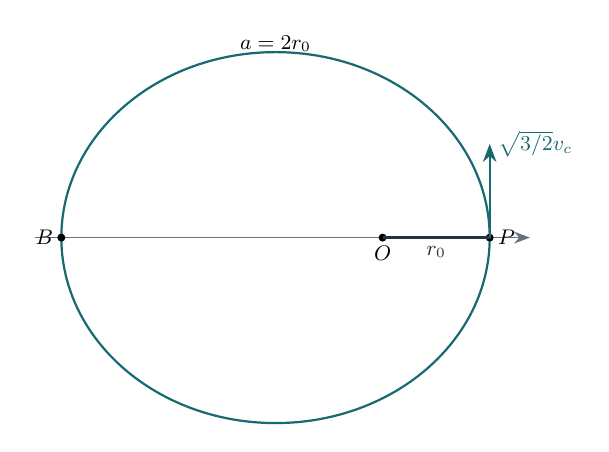
\begin{tikzpicture}[scale=0.85,transform shape]
\draw[axis] (-5.200000000000001,0)--(2.2,0);
\draw[traj] (-1.6,0) ellipse ({3.2} and {3.2*sqrt(1-0.5^2)});
\fill (0,0) circle (1.7pt) node[below] {$O$};
\fill (1.6,0) circle (1.7pt) node[right] {$P$};
\draw[object] (0,0)--(1.6,0) node[midway,below] {$r_0$};
\draw[motion] (1.6,0)--(1.6,1.4) node[right] {$\sqrt{3/2}v_c$};
\fill (-4.8,0) circle (1.7pt) node[left] {$B$};
\node at (-1.6,2.9) {$a=2r_0$};
\end{tikzpicture}
\figcaption{变图4.3V6\quad 给定比能量为圆轨道的一半，半长轴变成两倍初始半径。}
\end{minipage}\end{center}
\item 为什么逃逸速与圆速之比为 $\sqrt2$？变图4.3V7 以势能绝对值 $\mu m/r_0$ 为单位。圆轨道的动能为半个单位，零能逃逸的动能为一个单位。动能按速率平方变化，因此逃逸速是圆速的 $\sqrt2$ 倍。达到逃逸速后，引力仍持续向内做负功，速率在趋向无穷远的过程中降至零。
\begin{center}\begin{minipage}{.98\linewidth}\centering
\begin{tikzpicture}[scale=0.85,transform shape]
\draw[axis] (0,0)--(6.3,0) node[right] {状态};
\draw[axis] (0,0)--(0,3.2) node[above] {$K/(\mu m/r_0)$};
\fill[accent!20] (1,0) rectangle (2.1,1.25);\draw[object] (1,0) rectangle (2.1,1.25);
\fill[warm!20] (3.7,0) rectangle (4.8,2.5);\draw[object] (3.7,0) rectangle (4.8,2.5);
\node[above] at (1.55,1.25) {$1/2$};\node[above] at (4.25,2.5) {$1$};
\node[below] at (1.55,0) {圆轨道};\node[below] at (4.25,0) {零能逃逸};
\end{tikzpicture}
\figcaption{变图4.3V7\quad 同一位置的势能保持，零能逃逸需要两倍于圆轨道的动能。}
\end{minipage}\end{center}
\end{enumerate}

\clearpage

\pdfbookmark[2]{第 4 题 两质点万有引力相碰时间}{q4}

\section*{第 4 题\quad 两质点万有引力相碰时间}

\tagline{M-04-04}

空间中两质点质量分别为 $m_1,m_2$，仅以万有引力相互作用。开始时均静止，相距 $r_0$，随后相互靠近。求从释放到相碰所需的时间。按理想质点模型计算，相碰对应两者间距趋于零。

\par\medskip\noindent\begin{minipage}{\linewidth}\centering
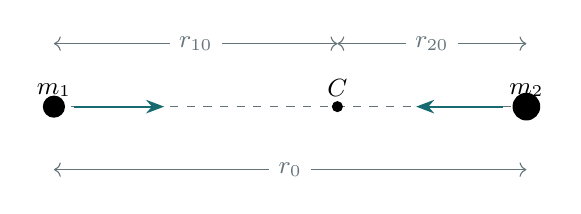
\begin{tikzpicture}[scale=1]

\draw[guide] (-3,0)--(3,0);\fill (-3,0) circle (4pt) node[above] {$m_1$};
\fill (3,0) circle (5pt) node[above] {$m_2$};\fill (.6,0) circle (2pt) node[above] {$C$};
\draw[motion] (-2.75,0)--(-1.6,0);\draw[motion] (2.7,0)--(1.6,0);
\draw[<->,muted] (-3,-.8)--(3,-.8) node[midway,fill=white] {$r_0$};
\draw[<->,muted] (-3,.8)--(.6,.8) node[midway,fill=white] {$r_{10}$};
\draw[<->,muted] (.6,.8)--(3,.8) node[midway,fill=white] {$r_{20}$};

\end{tikzpicture}
\figcaption{图 4.4　两质点同时向固定的质心 $C$ 运动。}
\end{minipage}\par\medskip

\Needspace{5\baselineskip}

\pdfbookmark[3]{题型定位}{q4-h0}

\subsection*{题型定位}

两体引力坠落时间可由相对运动的退化椭圆计算。两质点从静止相互靠近，等效引力参数为
\(G(m_1+m_2)\)，从最大距离到相碰对应半周期。

相对距离由 $r_0$ 缩至零，可视为退化椭圆从远端到近端的半周期。能量积分也给出同一时间，因为倒数速率在零间距端随 $\sqrt r$ 趋零。若物体有有限尺寸，积分下限取两表面接触时的质心间距。

\Needspace{5\baselineskip}

\pdfbookmark[3]{知识点}{q4-h1}

\subsection*{知识点}

\begin{itemize}
\tightlist
\item
  两体质心系
\item
  约化质量与相对运动
\item
  退化椭圆
\item
  开普勒第三定律
\item
  引力坠落时间
\end{itemize}

两个物体都向质心加速，两加速度相减后，相对距离的引力参数为 $G(m_1+m_2)$。固定中心近似则在一个质量远大于另一个质量时取得。能量先求相对速率，再积分距离得到相碰时间。质点模型在零距离速度发散，而时间积分仍可收敛；有限尺寸应改用非零接触距离。


\Needspace{5\baselineskip}

\pdfbookmark[3]{物理图像}{q4-h2}

\subsection*{物理图像}

两质点都向系统质心靠近，质心保持静止。相对坐标看，就是一个等效质点从距离
\(r_0\) 处由静止落向力心。

直线轨道可以想象成极扁的椭圆：远端在初始位置，近端退化到相碰点。初始静止点相当于椭圆远地点，从远地点到近地点需要半个周期。

解图4.4A中的两质点都向共同质心$C$移动，间距$r$由相对运动决定，引力参数为$G(m_1+m_2)$。解图4.4C在同一时间轴上画出间距从$r_0$降到零，释放端速度为零，末端速度发散，两端对总用时的贡献仍都有限。

\Needspace{5\baselineskip}

\pdfbookmark[3]{解题入口}{q4-h3}

\subsection*{解题入口}

以相对间距 $r$ 为坐标，两加速度相减得 $\ddot r=-G(m_1+m_2)/r^2$。从初态静止求相对速率，沿间距积分倒数速率得到用时。解图4.4B 的退化椭圆半长轴为 $r_0/2$，以半周期给出同一结果。

\Needspace{5\baselineskip}

\pdfbookmark[3]{标准解法}{q4-h4}

\subsection*{标准解法}

\subsubsection*{质心与相对运动}
系统不受外力，质心 $C$ 静止。设 $r=r_1+r_2$ 为相对距离，质心定义给出
\[
m_1r_1=m_2r_2,\qquad
r_1=\frac{m_2}{m_1+m_2}r,\quad
r_2=\frac{m_1}{m_1+m_2}r.
\]
\par\medskip\noindent\begin{minipage}{\linewidth}\centering
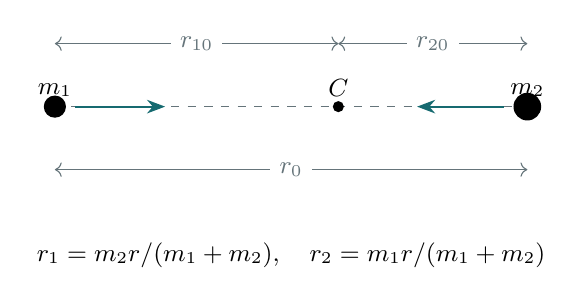
\begin{tikzpicture}[scale=1]

\draw[guide] (-3,0)--(3,0);\fill (-3,0) circle (4pt) node[above] {$m_1$};
\fill (3,0) circle (5pt) node[above] {$m_2$};\fill (.6,0) circle (2pt) node[above] {$C$};
\draw[motion] (-2.75,0)--(-1.6,0);\draw[motion] (2.7,0)--(1.6,0);
\draw[<->,muted] (-3,-.8)--(3,-.8) node[midway,fill=white] {$r_0$};
\draw[<->,muted] (-3,.8)--(.6,.8) node[midway,fill=white] {$r_{10}$};
\draw[<->,muted] (.6,.8)--(3,.8) node[midway,fill=white] {$r_{20}$};
\node[below] at (0,-1.6) {$r_1=m_2r/(m_1+m_2),\quad r_2=m_1r/(m_1+m_2)$};
\end{tikzpicture}
\figcaption{解图 4.4A　质心距离与相对距离。}
\end{minipage}\par\medskip

解图4.4A 中两段坠落距离按质量的反比分配。两质量相等时，质心在中点，两段距离各为 $r_0/2$。两加速度相减，得到相对距离的方程
\[
\ddot r=-\frac{Gm_2}{r^2}-\frac{Gm_1}{r^2}
=-\frac{\mu}{r^2},\qquad \mu=G(m_1+m_2).
\]
初态 $\dot r=0,r=r_0$，相对比能量为 $\varepsilon=-\mu/r_0$。与椭圆能量 $\varepsilon=-\mu/(2a)$ 比较，得 $a=r_0/2$。

\par\medskip\noindent\begin{minipage}{\linewidth}\centering
\begin{tikzpicture}[scale=1]
\draw[traj] (2.5,0) ellipse (2.5 and .55);\draw[guide] (0,0)--(5,0);
\fill (0,0) circle (2pt);\fill (5,0) circle (2pt);
\draw[guide] (0,0)--(0,-.85);\draw[guide] (5,0)--(5,-.85);
\node[below] at (0,-.85) {相碰端 $r=0$};\node[below] at (5,-.85) {释放端 $r=r_0$};
\draw[motion] (4.65,.28067)--(3.9,.55873);\node at (2.5,1.05) {$a=r_0/2,\quad t_c=T/2$};

\end{tikzpicture}
\figcaption{解图 4.4B　相对运动的椭圆取角动量趋零的极限。}
\end{minipage}\par\medskip

解图 4.4B 的椭圆在角动量趋零时退化为直线。释放端是远点，相碰端是近点极限，从远点到近点需要半周期：
\[
\boxed{t_c=\frac T2=\pi\sqrt{\frac{(r_0/2)^3}{G(m_1+m_2)}}
=\frac{\pi r_0^{3/2}}{2\sqrt{2G(m_1+m_2)}}}.
\]
也可跟踪 $m_1$ 本身。它到质心的初始距离 $r_{10}=m_2r_0/(m_1+m_2)$，受到的引力可改写为
\[
F_1=\frac{Gm_1m_2^3}{(m_1+m_2)^2r_1^2}
=\frac{Gm_1m^*}{r_1^2},\qquad
m^*=\frac{m_2^3}{(m_1+m_2)^2}.
\]
取这条退化轨道 $a_1=r_{10}/2$，由 $t_c=\pi\sqrt{a_1^3/(Gm^*)}$ 仍得相同答案。$m^*$ 是把两体运动改用单个质点的质心坐标描述时得到的等效参数。

\subsubsection*{由相对能量积分求相碰时间}
沿相对距离积分时，时间微元等于距离微元除以相对速率。由相对能量得到
\[
\frac12\dot r^2=\mu\left(\frac1r-\frac1{r_0}\right),
\qquad \dot r=-\sqrt{2\mu(1/r-1/r_0)}.
\]
故
\[
t_c=\int_0^{r_0}\frac{\dd r}{\sqrt{2\mu(1/r-1/r_0)}}.
\]
令 $r=r_0\sin^2\theta$，$0\leq\theta\leq\pi/2$，得到
\[
t_c=\frac{2r_0^{3/2}}{\sqrt{2\mu}}
 \int_0^{\pi/2}\sin^2\theta\,\dd\theta
=\frac{\pi r_0^{3/2}}{2\sqrt{2\mu}}.
\]
在 $r\to0$ 时瞬时速率和加速度发散，而倒数速率正比于 $\sqrt r$，所以时间积分收敛。若天体有有限尺寸，碰撞在两表面接触时发生，积分下限取该时刻的质心间距。
\subsubsection*{从释放到任意间距的完整时间关系}
为把解图4.4B的半周期与真实径向落体逐点对应，
令$r=r_0\cos^2\eta$，$\eta$从释放时的0增加到相碰时的$\pi/2$。
能量式给
\[
\dot r=-\sqrt{\frac{2\mu}{r_0}}\tan\eta,\qquad
\frac{\dd r}{\dd\eta}=-2r_0\sin\eta\cos\eta.
\]
二者相除，
\[
\frac{\dd t}{\dd\eta}
=\sqrt{\frac{2r_0^3}{\mu}}\cos^2\eta,
\]
\[
\boxed{t=\sqrt{\frac{r_0^3}{2\mu}}
(\eta+\sin\eta\cos\eta)},\qquad r=r_0\cos^2\eta.
\]
因此已落到间距$d$时，取$\eta=\arccos\sqrt{d/r_0}$，得到
\[
t(d)=\sqrt{\frac{r_0^3}{2\mu}}
\left[\arccos\sqrt{\frac d{r_0}}
+\sqrt{\frac d{r_0}\left(1-\frac d{r_0}\right)}\right].
\]
代$d=r_0$为零，代$d=0$为$t_c$；有限尺寸物体只须在实际接触间距停止积分。
解图4.4C按这个参数式画出全程，初端切线水平，末端切线趋于竖直，
初端速度为零，随后加速度随间距减小而增大，末端的竖直切线对应速率发散。用相对能量式积分得到这条非匀加速曲线。
\begin{center}\begin{minipage}{\linewidth}\centering
\begin{tikzpicture}[x=4cm,y=3cm]
\draw[axis](0,0)--(1.2,0)node[right]{$t/t_c$};
\draw[axis](0,0)--(0,1.2)node[above]{$r/r_0$};
\draw[traj,domain=0:90,samples=120]
 plot({2/pi*(rad(\x)+sin(\x)*cos(\x))},{cos(\x)^2});
\fill(0,1)circle(1.7pt);\fill(1,0)circle(1.7pt);
\node[left]at(0,1){$1$};\node[below]at(1,0){$1$};
\node[above right]at(.02,1){从静止释放};
\node[align=left,anchor=west]at(1.5,.75){$r=r_0\cos^2\eta$\\$\eta:0\to\pi/2$\\末段时间有限};
\end{tikzpicture}
\figcaption{解图4.4C\quad 两质点间距随时间收缩；曲线末端在有限时刻到达零，切线趋于竖直。}
\end{minipage}\end{center}

\subsubsection*{释放端和相碰端的积分阶数}
释放点$r\to r_0^-$时，
\[
\frac1r-\frac1{r_0}\sim\frac{r_0-r}{r_0^2},
\qquad \frac{\dd t}{|\dd r|}
\sim\frac{r_0}{\sqrt{2\mu}}(r_0-r)^{-1/2}.
\]
尽管初速为零，倒数速率在释放点发散，这一平方根奇点仍可积。
相碰点$r\to0^+$时，倒数速率正比于$\sqrt r$，也可积。
两个端点分别按 $(r_0-r)^{-1/2}$ 与 $r^{1/2}$ 积分，剩余时间都为有限值。

在最后一小段，积分剩余时间还给出
\[
t_c-t\sim\int_0^r\sqrt{\frac{s}{2\mu}}\,\dd s
=\frac{2r^{3/2}}{3\sqrt{2\mu}},
\]
\[
r\sim\left[\frac32\sqrt{2\mu}(t_c-t)\right]^{2/3}.
\]
所以速率按$(t_c-t)^{-1/3}$增长，而最后的间距按$(t_c-t)^{2/3}$缩短，
正好对应解图4.4C末端越来越陡的切线。
两质点各自的位置和速度始终按质心关系分配，在同一时刻到达质心 $C$。描述任一个质点时，路程和等效引力参数都由质心关系确定。令 $\alpha=m_2/(m_1+m_2)$，
则$r_1=\alpha r$、$r_{10}=\alpha r_0$，
等效引力参数为$Gm^*=\alpha^3\mu$，故
\[
\frac{r_{10}^3}{Gm^*}=\frac{\alpha^3r_0^3}{\alpha^3\mu}
=\frac{r_0^3}{\mu}.
\]
距离与等效参数中的质量比例恰好抵消，两个坐标描述的时间完全相同。
质心坐标把间距缩小为原来的 $\alpha$ 倍，同时把引力参数缩小为原来的 $\alpha^3$ 倍。这两项缩放在时间尺度中相消，因而每个质点的质心坐标与相对坐标都给出同一个相碰时刻。



\Needspace{5\baselineskip}

\pdfbookmark[3]{关键洞察}{q4-h5}

\subsection*{关键洞察}

退化椭圆把直线坠落纳入有心运动的周期框架。初始最大间距是长轴长度，因此半长轴是
\(r_0/2\)；相对引力参数包含两者的总质量。

接近相碰时，力和速率发散，倒数速率随 $\sqrt r$ 趋零，因此剩余时间有限。周期法和能量积分给出同一个相碰时刻。有限尺寸的物体在非零间距接触。

\Needspace{5\baselineskip}

\pdfbookmark[3]{易错点}{q4-h6}

\subsection*{易错点}

\begin{itemize}
\item 两物体都向共同质心移动，相对加速度包含两者的引力加速度。
\item 退化椭圆的长轴是最大间距 $r_0$，半长轴为 $r_0/2$。
\item 从远端到近端经过半周期。
\item 相对运动使用引力参数 $G(m_1+m_2)$。
\item 两质点到质心的距离按质量反比分配，等质量时才各为 $r_0/2$。
\item 质心坐标与相对坐标中的距离和等效引力参数同时缩放，保持同一时间尺度。
\end{itemize}

\Needspace{5\baselineskip}

\pdfbookmark[3]{课堂讲解建议}{q4-h7}

\subsection*{课堂讲解建议}

先用解图4.4A 问两质点到质心的距离如何分配，由 $m_1r_1=m_2r_2$ 得质量反比。再在相对方程中标出两加速度，解释总质量出现在引力参数中。对变图4.4V5，从释放点沿曲线读到 $r=r_0/2$，计算对应时间占全程的比例，说明坠落后半段因速度较大而用时较少。

\Needspace{5\baselineskip}

\pdfbookmark[3]{变式训练}{q4-h8}

\subsection*{变式训练}

\begin{enumerate}
\item 令 $m_2\gg m_1$。变图4.4V1 中，质心靠近较重物体，较轻物体到质心的距离近似为 $r_0$。相对引力参数 $\mu=G(m_1+m_2)\simeq Gm_2$，于是 $t_c\simeq\pi\sqrt{r_0^3/(8Gm_2)}$，与从静止落向固定中心的时间相同。该近似同时体现在质心距离与相对加速度两处。
\begin{center}\begin{minipage}{.98\linewidth}\centering
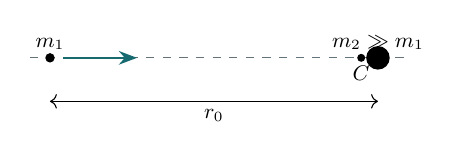
\begin{tikzpicture}[scale=0.85,transform shape]
\draw[guide] (-2.8,0)--(2.8,0);
\fill (-2.5,0) circle (2pt) node[above] {$m_1$};
\fill (2.4,0) circle (5pt) node[above] {$m_2\gg m_1$};
\fill (2.15,0) circle (1.7pt) node[below] {$C$};
\draw[motion] (-2.3,0)--(-1.2,0);
\draw[<->] (-2.5,-.65)--(2.4,-.65) node[midway,below] {$r_0$};
\end{tikzpicture}
\figcaption{变图4.4V1\quad 大质量物体接近质心，较轻的物体承担几乎全部相对位移。}
\end{minipage}\end{center}
\item 初距改为 $2r_0$，两质量保持。变图4.4V2 的两种初态都从静止释放，公式中的质量参数相同，只有初距改变。因此时间之比为 $(2r_0)^{3/2}/r_0^{3/2}=2\sqrt2$。初距增大时，引力初加速度更小，时间增长快于初距的线性比例。
\begin{center}\begin{minipage}{.98\linewidth}\centering
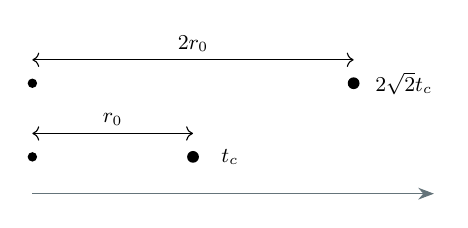
\begin{tikzpicture}[scale=0.85,transform shape]
\draw[axis] (0,0)--(6,0);
\foreach \y/\end/\txt in {.55/2.4/r_0,1.65/4.8/{2r_0}} {
  \fill (0,\y) circle (2pt);\fill (\end,\y) circle (2.5pt);
  \draw[<->] (0,{\y+.35})--(\end,{\y+.35}) node[midway,above] {$\txt$};}
\node[right] at (2.7,.55) {$t_c$};\node[right] at (5,1.65) {$2\sqrt2t_c$};
\end{tikzpicture}
\figcaption{变图4.4V2\quad 初距加倍、两质量保持时，相碰时间按距离的 $3/2$ 次方增长。}
\end{minipage}\end{center}
\item 初态增加向内相对速率 $w$。由能量守恒，
\[
\dot r=-\sqrt{w^2+2\mu(1/r-1/r_0)},\qquad
t=\int_0^{r_0}\frac{\dd r}{\sqrt{w^2+2\mu(1/r-1/r_0)}}.
\]
变图4.4V3 的实线从 $r/r_0=1$ 处的非零速率开始，在每个间距都高于静止释放曲线，因此所需时间较短。初始比能量为 $w^2/2-\mu/r_0$。当 $0<w<\sqrt{2\mu/r_0}$ 时，退化椭圆的远端大于 $r_0$，从其半周期扣除由远端落到 $r_0$ 的时间。达到或超过 $\sqrt{2\mu/r_0}$ 时，直接用上面的径向积分计算从 $r_0$ 到相碰的时间。
\begin{center}\begin{minipage}{.98\linewidth}\centering
\begin{tikzpicture}[scale=0.85,transform shape]
\draw[axis] (0,0)--(5.8,0) node[right] {$r/r_0$};
\draw[axis] (0,0)--(0,3.7) node[above] {$|\dot r|/\sqrt{\mu/r_0}$};
\draw[traj,domain=.2:1,samples=70] plot ({5*\x},{sqrt(1+2*(1/\x-1))});
\draw[guide,domain=.2:1,samples=70] plot ({5*\x},{sqrt(2*(1/\x-1))});
\fill (5,1) circle (1.7pt) node[right] {$w=\sqrt{\mu/r_0}$};
\fill (5,0) circle (1.7pt) node[above left] {$w=0$};
\node[below] at (5,0) {$1$};
\end{tikzpicture}
\figcaption{变图4.4V3\quad 给定向内初速后，各间距处的相对速率都高于从静止释放的值。}
\end{minipage}\end{center}
\item 从相对能量的倒数速率积分重求时间。令 $r=r_0\sin^2\theta$，则 $\dd r=2r_0\sin\theta\cos\theta\dd\theta$，而速率大小是 $\sqrt{2\mu/r_0}\cot\theta$。约去共同因子得
\[
t_c=\frac{2r_0^{3/2}}{\sqrt{2\mu}}\int_0^{\pi/2}\sin^2\theta\dd\theta
=\frac{\pi r_0^{3/2}}{2\sqrt{2\mu}}.
\]
变图4.4V4 的阴影面积为 $\pi/4$。变量替换后两个端点都给有限积分。
\begin{center}\begin{minipage}{.98\linewidth}\centering
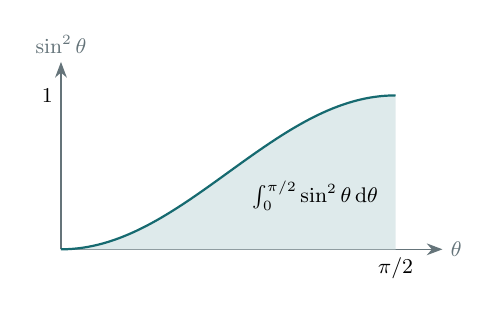
\begin{tikzpicture}[scale=0.85,transform shape]
\draw[axis] (0,0)--(5.7,0) node[right] {$\theta$};
\draw[axis] (0,0)--(0,2.8) node[above] {$\sin^2\theta$};
\fill[accent!14,domain=0:90,samples=65] (0,0)--plot ({\x/18},{2.3*sin(\x)^2})--(5,0)--cycle;
\draw[traj,domain=0:90,samples=65] plot ({\x/18},{2.3*sin(\x)^2});
\node[below] at (5,0) {$\pi/2$};\node[left] at (0,2.3) {$1$};
\node at (3.8,.8) {$\int_0^{\pi/2}\sin^2\theta\dd\theta$};
\end{tikzpicture}
\figcaption{变图4.4V4\quad 用 $r=r_0\sin^2\theta$ 后，碰撞时间积分转为有限的正弦平方积分。}
\end{minipage}\end{center}
\item 只落到间距 $d>0$。变图4.4V5 中，取 $z=d/r_0$，用 $r=r_0\cos^2\eta$ 得 $\eta=\arccos\sqrt z$。代入积分，
\[
t(d)=\sqrt{\frac{r_0^3}{2\mu}}\left[\arccos\sqrt z+\sqrt{z(1-z)}\right].
\]
$d\to0$ 时回到 $t_c$，$d=r_0$ 时为零。图中 $d=r_0/2$ 给 $t/t_c=1/2+1/\pi\approx0.8183$，后半程间距只用了约 $0.1817t_c$。
\begin{center}\begin{minipage}{.98\linewidth}\centering
\begin{tikzpicture}[scale=0.85,transform shape]
\draw[axis] (0,0)--(5.8,0) node[right] {$t/t_c$};
\draw[axis] (0,0)--(0,3.1) node[above] {$r/r_0$};
\draw[traj,domain=0:90,samples=80] plot ({5*2/pi*(rad(\x)+sin(\x)*cos(\x))},{2.6*cos(\x)^2});
\pgfmathsetmacro{\xhalf}{5*(.5+1/pi)}
\draw[guide] (0,1.3)--(\xhalf,1.3)--(\xhalf,0);
\fill (\xhalf,1.3) circle (1.7pt) node[right] {$r=d=r_0/2$};
\node[below] at (5,0) {$1$};\node[left] at (0,1.3) {$1/2$};
\end{tikzpicture}
\figcaption{变图4.4V5\quad 图中点表示只落到一半间距，用时超过总相碰时间的一半。}
\end{minipage}\end{center}
\item 给初态一个小的横向速率 $0<w_t<\sqrt{\mu/r_0}$。令 $q=w_t^2r_0/\mu$，初点是远点，$a=r_0/(2-q)$、$e=1-q$。变图4.4V6 的正近点半径为 $r_{\min}=a(1-e)=qr_0/(2-q)>0$。所以理想质点在到达正间距后转向。有限尺寸物体若接触间距为 $d$，则以 $r_{\min}\le d$ 判断是否发生表面接触。
\begin{center}\begin{minipage}{.98\linewidth}\centering
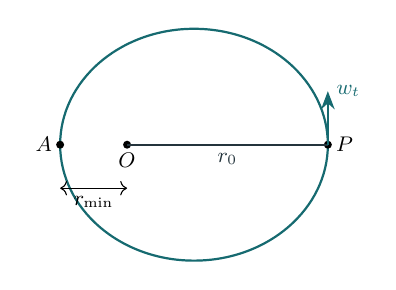
\begin{tikzpicture}[scale=0.85,transform shape]
\draw[traj] (1,0) ellipse (2 and 1.732051);
\fill (0,0) circle (1.7pt) node[below] {$O$};
\fill (3,0) circle (1.7pt) node[right] {$P$};
\fill (-1,0) circle (1.7pt) node[left] {$A$};
\draw[object] (0,0)--(3,0) node[midway,below] {$r_0$};
\draw[motion] (3,0)--(3,.8) node[right] {$w_t$};
\draw[<->] (-1,-.65)--(0,-.65) node[midway,below] {$r_{\min}$};
\end{tikzpicture}
\figcaption{变图4.4V6\quad 小横向初速保留角动量，理想质点在正的最小间距处转向。}
\end{minipage}\end{center}
\item 由量纲分析相碰时间。引力参数的量纲为 $[\mu]=\mathrm{L^3T^{-2}}$，和初距 $r_0$ 组合得到时间尺度 $\sqrt{r_0^3/\mu}$。变图4.4V7 以任意固定长度 $\ell$ 归一化，曲线为 $t_c/\sqrt{\ell^3/\mu}=[\pi/(2\sqrt2)](r_0/\ell)^{3/2}$。其中无量纲系数 $\pi/(2\sqrt2)$ 来自能量积分，量纲关系本身只给尺度。
\begin{center}\begin{minipage}{.98\linewidth}\centering
\begin{tikzpicture}[scale=0.85,transform shape]
\draw[axis] (0,0)--(5.4,0) node[right] {$r_0/\ell$};
\draw[axis] (0,0)--(0,3.5) node[above] {$t_c/\sqrt{\ell^3/\mu}$};
\draw[traj,domain=0:2.1,samples=60] plot ({2.1*\x},{.9*pi/(2*sqrt(2))*\x^1.5});
\draw[guide] (2.1,0)--(2.1,{.9*pi/(2*sqrt(2))});
\node[below] at (2.1,0) {$1$};\node[right] at (2.1,{.9*pi/(2*sqrt(2))}) {$\pi/(2\sqrt2)$};
\end{tikzpicture}
\figcaption{变图4.4V7\quad 量纲给出时间尺度，曲线上的系数由动力学积分确定。}
\end{minipage}\end{center}
\end{enumerate}

\clearpage

\pdfbookmark[2]{第 5 题 绕月飞船两种登月喷气方案}{q5}

\section*{第 5 题\quad 绕月飞船两种登月喷气方案}

\tagline{M-04-05}

质量 $m=1.20\times10^4\,\mathrm{kg}$ 的飞船在月面上方 $h=100\,\mathrm{km}$ 的圆轨道运动。采用以下两种方式使轨道与月面相切：
\begin{enumerate}
\item 在 $A$ 向运动前方短时喷气，使飞船在 $B$ 与月面相切，$A,O,B$ 共线，$O$ 为月心。
\item 在 $A$ 沿径向向外短时喷气，使飞船在 $C$ 与月面相切，$OC\perp OA$。
\end{enumerate}
喷气相对飞船的速率恒为 $u=1.00\times10^4\,\mathrm{m/s}$；忽略喷气期间引力的冲量。月球半径 $R=1700\,\mathrm{km}$，月面重力加速度 $g=1.700\,\mathrm{m/s^2}$，月外引力遵从平方反比律。求两方案的速度改变量与燃料质量。月面相切只表示轨道到达条件，不包含软着陆制动。

\par\medskip\noindent\begin{minipage}{\linewidth}\centering
\begin{tikzpicture}[scale=.86]
\draw[object,fill=rulegray!25](0,0)circle(2.55);\draw[guide](0,0)circle(2.7);
\fill(0,0)circle(2pt);\node[below]at(0,0){$O$};
\fill(2.7,0)circle(2pt);\node[below right]at(2.7,0){$A$};
\draw[object](0,0)--(2.7,0)node[midway,below]{$R+h$};
\draw[motion](2.7,0)--(2.7,1.2)node[right]{$v_0$};
\fill(-2.55,0)circle(1.8pt);\node[left]at(-2.55,0){$B$};
\fill(0,2.55)circle(1.8pt);\node[above left]at(0,2.55){$C$};
\draw[guide](-2.55,0)--(0,0)--(0,2.55);\node at(-1,-1){月球};
\end{tikzpicture}
\figcaption{图4.5\quad 按$R:h=17:1$绘图；$B$、$C$分别是两种方案要求的月面相切点。}
\end{minipage}\par\medskip

\Needspace{5\baselineskip}

\pdfbookmark[3]{题型定位}{q5-h0}

\subsection*{题型定位}

短时喷气变轨与燃料计算。先由月面相切条件确定新椭圆，再求速度矢量改变量，最后按排气模型计算燃料质量。轨道阶段与燃烧阶段使用的守恒对象不同。

切向减速改变比角动量，喷气点成为远月点；径向脉冲保留切向分量，喷气点不是拱点。两方案分别由近点位置和角动量条件确定脉冲的方向与大小。连续排气的相对速率定义决定燃料方程。

\Needspace{5\baselineskip}

\pdfbookmark[3]{知识点}{q5-h1}

\subsection*{知识点}

\begin{itemize}
\tightlist
\item
  圆轨道速度
\item
  短时喷气近似动量守恒
\item
  椭圆轨道近远点条件
\item
  角动量与机械能守恒
\item
  连续排气火箭方程与燃料质量
\end{itemize}

短时喷气改变速度，新的能量和角动量决定轨道与月面的相切位置。径向脉冲和切向脉冲分别改变速度的不同分量，燃料量由火箭方程求出。若要求软着陆，还需在相切点另算制动所需的速度改变量。


\Needspace{5\baselineskip}

\pdfbookmark[3]{物理图像}{q5-h2}

\subsection*{物理图像}

A 点是原圆轨道上的一点。切向喷气后，飞船速度方向仍切向，A
点会成为新椭圆的一个拱点；若新轨道与月球在 B 点相切，A、B 与月心共线。

径向喷气后，飞船在 A 点获得径向速度，A 点不再是拱点；飞船沿椭圆到 C
点与月面相切。此时轨道几何比第一种更隐蔽，需要同时用能量和角动量。

解图4.5A在$A$沿切向减速，解图4.5B在同一位置加向内径向分量；两种脉冲分别沿切向与径向，所需燃料由各自速度矢量改变量的大小决定。脉冲期间月球引力冲量可略，喷气后才分别使用固定的轨道能量与角动量；两条轨道均以$O$为焦点并与月面相切。

\Needspace{5\baselineskip}

\pdfbookmark[3]{解题入口}{q5-h3}

\subsection*{解题入口}

先求引力参数 $\mu=gR^2$ 与当地圆速 $v_0$。切向方案由两拱点 $R+h,R$ 求新椭圆的远点速度；径向方案保留角动量，用月面相切点的速度和能量求向内分量。随后分别将这两支速度矢量改变量的大小代入连续排气的火箭方程。

\Needspace{5\baselineskip}

\pdfbookmark[3]{标准解法}{q5-h4}

\subsection*{标准解法}

\subsubsection*{原圆轨道}
月面 $g$ 只用于确定引力参数；飞船所在高度的引力加速度仍随 $r^{-2}$ 变化：
\[
\mu=GM=gR^2,\qquad r_A=R+h,\qquad
v_0=\sqrt{\frac\mu{R+h}}=1652.10\,\mathrm{m/s}.
\]
求燃料之前，先分别求轨道所需的速度矢量改变量。

\subsubsection*{方案一：切向减速}
\par\medskip\noindent\begin{minipage}{\linewidth}\centering
\begin{tikzpicture}[scale=.86]
\draw[object,fill=rulegray!25](0,0)circle(2.55);\draw[guide](0,0)circle(2.7);
\draw[traj](.075,0)ellipse(2.625 and 2.623928353);
\fill(0,0)circle(2pt);\node[below]at(0,0){$O$};
\fill(2.7,0)circle(2pt);\node[below right]at(2.7,0){$A$};
\fill(-2.55,0)circle(2pt);\node[left]at(-2.55,0){$B$};
\draw[motion](2.7,0)--(2.7,1)node[right]{$v_0$};
\draw[motion](3.45,0)--(3.45,.98561)node[right]{$v_A$};
\draw[motion](-2.55,0)--(-2.55,-1.04365)node[left]{$v_B$};
\draw[force](2.7,1.5)--(2.7,2.2)node[right]{向前排气};
\draw[object](0,0)--(2.7,0)node[midway,below]{$R+h$};
\end{tikzpicture}
\figcaption{解图4.5A\quad 轨道按实际高度比例绘制，$O$是椭圆焦点；$A$为远月点、$B$为近月点。}
\end{minipage}\par\medskip

解图 4.5A 中，向前排气使飞船反冲减速，$A$ 成为远月点，$B$ 为近月点。燃烧后飞船质量虽已减少，在轨道方程两边可以约去。设两点速度为 $v_A,v_B$，有
\[
(R+h)v_A=Rv_B,\qquad
\frac12v_A^2-\frac\mu{R+h}
=\frac12v_B^2-\frac\mu R.
\]
代入 $v_B=(R+h)v_A/R$，整理为
\[
v_A^2\left[\frac{(R+h)^2}{R^2}-1\right]
=2\mu\left(\frac1R-\frac1{R+h}\right).
\]
从而
\[
v_A=\sqrt{\frac{2gR^3}{(R+h)(2R+h)}}=1628.33\,\mathrm{m/s},
\quad v_B=\frac{R+h}{R}v_A=1724.11\,\mathrm{m/s}.
\]
所需反向切向速度改变量大小为
\[
\Delta v_1=v_0-v_A=23.77\,\mathrm{m/s}.
\]

\subsubsection*{方案二：向内径向脉冲}
\par\medskip\noindent\begin{minipage}{\linewidth}\centering
\begin{tikzpicture}[scale=.86]
\draw[object,fill=rulegray!25](0,0)circle(2.55);\draw[guide](0,0)circle(2.7);
\draw[traj](0,-.159375)ellipse(2.704683438 and 2.709375);
\fill(0,0)circle(2pt);\node[below]at(0,0){$O$};
\fill(2.7,0)circle(2pt);\node[below right]at(2.7,0){$A$};
\fill(0,2.55)circle(2pt);\node[above left]at(0,2.55){$C$};
\draw[object](0,0)--(2.7,0)node[midway,below]{$R+h$};
\draw[motion](2.7,0)--(2.629411765,1.2)node[above right]{$\vect v_A$};
\draw[force](2.7,0)--(3.7,0)node[above]{向外排气};
\node[align=left,anchor=west]at(4.6,1.3){$v_{A,r}=-\Delta v_2$\\$v_{A,\varphi}=v_0$\\$e=h/R=1/17$};
\end{tikzpicture}
\figcaption{解图4.5B\quad 向内径向脉冲后的真实比例椭圆，$O$为上焦点，速度箭头沿$A$处切线。}
\end{minipage}\par\medskip

解图 4.5B 中排气向外，飞船获得向内速度 $-\Delta v_2\vect e_r$，切向分量仍为 $v_0$，故
\[
v_A^2=v_0^2+\Delta v_2^2,\qquad
h_{\rm orb}=(R+h)v_0=Rv_C.
\]
脉冲只增加径向分量，飞船的比角动量保持为 $h_{\rm orb}$，比能量增加 $\Delta v_2^2/2$。在脉冲后的轨道上，由比能量守恒，
\[
\frac12(v_0^2+\Delta v_2^2)-\frac\mu{R+h}
=\frac12v_C^2-\frac\mu R,
\quad v_C=\frac{R+h}R v_0.
\]
用 $\mu=(R+h)v_0^2$ 消去引力参数，得到
\[
\begin{aligned}
\Delta v_2^2
&=\left[\frac{(R+h)^2}{R^2}-1\right]v_0^2
 -2\mu\left(\frac1R-\frac1{R+h}\right)\\
&=\left(\frac hR\right)^2v_0^2.
\end{aligned}
\]
因此
\[
\Delta v_2=\frac hR v_0=97.18\,\mathrm{m/s},\qquad
v_C=1749.29\,\mathrm{m/s},\quad v_A=1654.96\,\mathrm{m/s}.
\]
月面相切点 $C$ 满足 $OC\perp OA$。此轨道半通径为 $p=h_{\rm orb}^2/\mu=R+h$，近点为 $r_C=R=p/(1+e)$，故 $e=h/R$。$A$ 的距离为 $p$，对应近点极角 $\varphi=-\pi/2$，并因径向速度向内沿轨道到达 $C$；几何条件与速度符号一致。

\subsubsection*{燃料质量与喷气模型}
对题设恒定相对排气速率，令飞船当前质量为 $m_s$，喷出少量燃料 $\dd m_{\rm e}=-\dd m_s>0$。忽略外力冲量，沿推力方向的微元动量关系为
\[
m_s\,\dd v=u\,\dd m_{\rm e}=-u\,\dd m_s.
\]
积分得 $\Delta v=u\ln(m/m_f)$，这里 $m_f$ 表示燃烧结束的飞船质量。因此两方案燃料量为
\[
\boxed{\Delta m_i=m\left(1-e^{-\Delta v_i/u}\right)},
\qquad \Delta m_1=28.49\,\mathrm{kg},\quad
\Delta m_2=116.05\,\mathrm{kg}.
\]
由于 $\Delta v_i/u\ll1$，一阶近似 $\Delta m_i\simeq m\Delta v_i/u$ 分别给出 $28.53\,\mathrm{kg}$ 和 $116.62\,\mathrm{kg}$。

若另采用“全部燃料一次抛出”的集中模型，并把排气速度 $u$ 定义为相对\emph{喷气前}飞船的速度，则动量关系分别是
\[
mv_0=(m-\Delta m)v_A+\Delta m(v_0+u),\qquad
0=\Delta m u-(m-\Delta m)\Delta v_2.
\]
它们给出 $\Delta m=m\Delta v/(u+\Delta v)$，数值为 $28.46\,\mathrm{kg}$、$115.50\,\mathrm{kg}$。这一集中排气模型将 $u$ 约定为相对燃烧前的飞船速度。题设的连续模型则逐微元以当时飞船为参照，积分给出指数形式的燃料量。两种估算都表明切向减速所需燃料明显较少。飞船到月面仍有约 $1.7\,\mathrm{km/s}$ 的切向速度，后续软着陆需另行制动。
\subsubsection*{两种脉冲的速度矢量改变量}
解图4.5A中切向减速，$\Delta\vect v_1$与初速度反向；
解图4.5B中径向脉冲则与初速度垂直。
因此两次喷气对比机械能的改变分别是
\[
\Delta\varepsilon_1=-v_0\Delta v_1+\frac12\Delta v_1^2,
\qquad
\Delta\varepsilon_2=\frac12\Delta v_2^2.
\]
第二种方案的脉冲方向垂直于原速度。两支速度矢量之差的大小为 $97.18\,\mathrm{m/s}$，这个量进入燃料方程。喷气前后两速率相减只得到约 $2.86\,\mathrm{m/s}$，它描述的是速率增加了多少。

两幅新椭圆均以$O$为焦点，最小半径为$R$，所以从$A$到指定接触点之前不会先穿入月面。
在 $B$、$C$ 的到达速度分别为 $v_B$、$v_C$，沿各自的月面切线。若还要求着陆时的速度为零，应在相切点另加与到达速度反向的制动脉冲。
在解图4.5B 将径向脉冲改为向外，能量和比角动量的数值保持，近、远月点的距离也保持。径向速度反号使近点方向关于 $OA$ 镜像，新的相切点位于 $OC$ 朝下的延长线上。


\Needspace{5\baselineskip}

\pdfbookmark[3]{关键洞察}{q5-h5}

\subsection*{关键洞察}

燃料量由速度矢量改变量的大小确定。径向方案中，两支长速度箭头近乎平行，仍需向内的径向增量。切向减速改变角动量，使较小的脉冲足以降低近点。
轨道运动使用比能量和比角动量，飞船质量可约去。连续排气时质量在燃烧期间减少，积分给指数形式的燃料量。若将排气视为一次抛出，相对速率按约定的燃烧前状态定义，得到另一条动量式；两模型在小消耗时有相同的一阶近似。

\Needspace{5\baselineskip}

\pdfbookmark[3]{易错点}{q5-h6}

\subsection*{易错点}

\begin{itemize}
\item 喷气期间燃料带走动量和能量，喷气后的轨道以新的速度为初态。
\item 径向脉冲后 $A$ 点的径向速度非零，位于两拱点之间。
\item 排气速率 $u$ 与飞船所需速度增量通过火箭方程相连。
\item 月面相切点处速度垂直当地半径，半径取 $R$。
\item 切向与径向方案分别确定新的角动量和轨道几何。
\item 速度矢量之差的大小进入燃料方程。
\item 小燃料量近似以 $\Delta v/u\ll1$ 为条件。
\item 月外引力加速度随半径平方反比，月面重力用于求 $GM=gR^2$。
\item 相切点仍有切向速度，软着陆另需制动。
\end{itemize}

\Needspace{5\baselineskip}

\pdfbookmark[3]{课堂讲解建议}{q5-h7}

\subsection*{课堂讲解建议}

在解图4.5A 和B 先画排气方向，再画飞船所受反冲。问为什么径向方案的速度改变量大于其速率增加，由变图4.5V4 的两支近乎平行长箭头和短径向箭头回答。随后用 $p=R+h$、$r_C=p/(1+e)$ 推得 $e=h/R$，说明 $A,C$ 的相对角度。最后按微元动量式积分燃料量，保留到达月面时约 $1.7\,\mathrm{km/s}$ 的速度供后续制动讨论。

\Needspace{5\baselineskip}

\pdfbookmark[3]{变式训练}{q5-h8}

\subsection*{变式训练}

\begin{enumerate}
\item 将喷气方向反转。第一方案向后排气，飞船获得正切向增量，速率高于当地圆速，故变图4.5V1 的 $A$ 成为近点，远点升高。第二方案向内排气，飞船获得向外的径向速度。其速率平方与角动量和原径向方案相同，所以两拱点距离保持，但径向速度符号反向，使椭圆关于 $OA$ 镜像。近月点由图中的 $C$ 转到另一侧的 $C'$。
\begin{center}\begin{minipage}{.98\linewidth}\centering
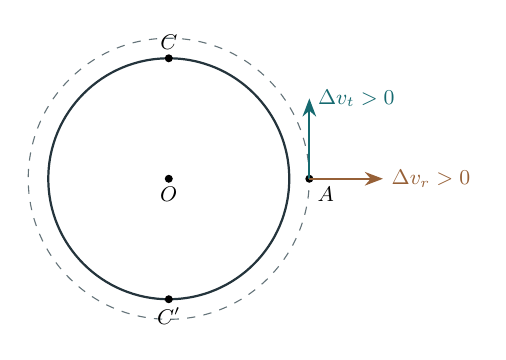
\begin{tikzpicture}[scale=0.85,transform shape]
\draw[object] (0,0) circle (1.8);\draw[guide] (0,0) circle (2.1);
\fill (0,0) circle (1.7pt) node[below] {$O$};\fill (2.1,0) circle (1.7pt) node[below right] {$A$};
\draw[motion] (2.1,0)--(2.1,1.2) node[right] {$\Delta v_t>0$};
\draw[force] (2.1,0)--(3.2,0) node[right] {$\Delta v_r>0$};
\fill (0,1.8) circle (1.7pt) node[above] {$C$};
\fill (0,-1.8) circle (1.7pt) node[below] {$C'$};
\end{tikzpicture}
\figcaption{变图4.5V1\quad 反向排气分别使切向加速或径向向外反冲，后者使近月点转至 $C'$。}
\end{minipage}\end{center}
\item 改变高度，求 $h\ll R$ 时的速度改变量。令 $\eta=h/R$，切向方案给 $v_A/v_0=\sqrt{2/(2+\eta)}=(1+\eta/2)^{-1/2}=1-\eta/4+O(\eta^2)$。故 $\Delta v_1=\eta v_0/4+O(\eta^2v_0)$，而径向方案精确为 $\Delta v_2=\eta v_0$。变图4.5V2 的原点附近两条线的斜率分别为 $1/4$ 和 $1$。同时 $v_0\to\sqrt{gR}$，径向方案所需速度改变量约为切向的四倍。
\begin{center}\begin{minipage}{.98\linewidth}\centering
\begin{tikzpicture}[scale=0.85,transform shape]
\draw[axis] (0,0)--(6.3,0) node[right] {$h/R$};\draw[axis] (0,0)--(0,3.35) node[above] {$\Delta v/v_0$};
\draw[traj,domain=0:.2,samples=65] plot ({28*\x},{14*(1-sqrt(2/(2+\x)))});
\draw[force,domain=0:.2,samples=65] plot ({28*\x},{14*\x});
\node[right] at (5.6,2.8) {径向};\node[right] at (5.6,{14*(1-sqrt(2/2.2))}) {切向};
\node[below] at (2.8,0) {$0.1$};
\end{tikzpicture}
\figcaption{变图4.5V2\quad 低轨极限中，两方案速度改变量均随高度线性增加，径向的斜率为切向的四倍。}
\end{minipage}\end{center}
\item 提高排气速率 $u$，保持轨道要求的 $\Delta v$ 不变。燃料分数为 $f=1-e^{-\Delta v/u}$，对 $u$ 求导得 $\dd f/\dd u=-(\Delta v/u^2)e^{-\Delta v/u}<0$。变图4.5V3 因而单调下降。当 $\Delta v/u\ll1$ 时，$f=\Delta v/u+O[(\Delta v/u)^2]$，燃料量近似与 $u$ 成反比。
\begin{center}\begin{minipage}{.98\linewidth}\centering
\begin{tikzpicture}[scale=0.85,transform shape]
\draw[axis] (0,0)--(6.5,0) node[right] {$u/\Delta v$};\draw[axis] (0,0)--(0,3.3) node[above] {$\Delta m/m$};
\draw[traj,domain=.5:8,samples=65] plot ({.72*\x},{3*(1-exp(-1/\x))});
\node[below] at (1.44,0) {$2$};
\fill (1.44,{3*(1-exp(-.5))}) circle (1.7pt) node[above right] {$1-e^{-1/2}$};
\end{tikzpicture}
\figcaption{变图4.5V3\quad 固定轨道所需的速度改变量，提高排气速率会降低燃料分数。}
\end{minipage}\end{center}
\item 只用速度矢量说明燃料需求。切向方案取 $\Delta\vect v_1=-\Delta v_1\vect e_\varphi$，径向方案取 $\Delta\vect v_2=-\Delta v_2\vect e_r$。变图4.5V4 用 $h/R=1/17$ 画径向方案，$|\vect v_A|=\sqrt{v_0^2+\Delta v_2^2}$。因此速率增加为 $v_0[\sqrt{1+(h/R)^2}-1]$，是高度比的二阶量；速度矢量的改变量仍是一阶的 $(h/R)v_0$，其方向指向月心。
\begin{center}\begin{minipage}{.98\linewidth}\centering
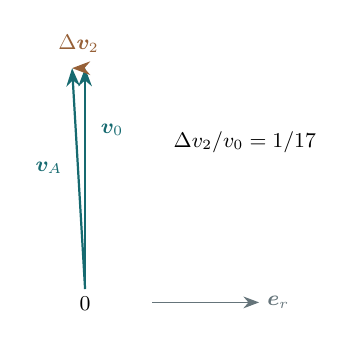
\begin{tikzpicture}[scale=0.85,transform shape]
\coordinate (A) at (0,0);\coordinate (V0) at (0,3.3);\coordinate (V2) at ({-3.3/17},3.3);
\draw[motion] (A)--(V0) node[pos=.72,right=3pt] {$\vect v_0$};
\draw[force] (V0)--(V2) node[midway,above=3pt] {$\Delta\vect v_2$};
\draw[motion] (A)--(V2) node[pos=.55,left=3pt] {$\vect v_A$};
\draw[axis] (1,-.2)--(2.6,-.2) node[right] {$\vect e_r$};
\node[below] at (0,0) {$0$};
\node[right] at (1.2,2.2) {$\Delta v_2/v_0=1/17$};
\end{tikzpicture}
\figcaption{变图4.5V4\quad 径向方案的矢量改变量与初速垂直，两长箭头的长度之差远小于短径向箭头。}
\end{minipage}\end{center}
\item 换一个喷气点，怎样进入给定相切轨道？变图4.5V5 固定目标椭圆的 $p,e$，其比能量为 $\varepsilon=-\mu(1-e^2)/(2p)$。以图中 $OA$ 为极轴，$\varphi$ 逆时针为正，当前位置 $P$ 满足 $r=p/(1+e\cos\varphi)$。沿图中箭头飞行时，比角动量为 $h_{\rm orb}=\sqrt{\mu p}$。由 $v_\varphi=r\dot\varphi$、$\dot\varphi=h_{\rm orb}/r^2$，并对 $1/r$ 求导，得到
\[
v_\varphi=\frac{\sqrt{\mu p}}r,\qquad
v_r=-h_{\rm orb}\frac{\dd(1/r)}{\dd\varphi}
=e\sqrt{\frac{\mu}{p}}\sin\varphi.
\]
由能量式也能得到径向速率 $|v_r|=\sqrt{2(\varepsilon+\mu/r)-\mu p/r^2}$。方向由所在点和运行方向共同确定。图示 $P$ 在 $0<\varphi<\pi$ 一侧，此时沿箭头从近点 $A$ 向远点 $B$ 飞行，$v_r>0$；沿同一椭圆反向飞行时，两个速度分量一同反号。目标速度减去当地喷气前速度，即为所需脉冲。若限制只能径向或切向喷气，另一个分量应当已经与目标值相同。
\begin{center}\begin{minipage}{.98\linewidth}\centering
\begin{tikzpicture}[scale=0.85,transform shape]
\pgfmathsetmacro{\bb}{2.5*sqrt(1-0.4^2)}
\draw[traj] (0,0) ellipse (2.5 and \bb);
\coordinate (O) at ({2.5*0.4},0);\coordinate (C) at (0,0);
\fill (O) circle (1.7pt) node[below] {$O$};
\fill (C) circle (1.4pt) node[below left] {$C$};
\fill (2.5,0) circle (1.6pt) node[right] {$A$};
\fill (-2.5,0) circle (1.6pt) node[left] {$B$};
\coordinate (P) at ({2.5*cos(45)},{2.5*sqrt(.84)*sin(45)});
\fill (P) circle (1.7pt) node[above right] {$P$};
\draw[object] (O)--(P) node[midway,right] {$r$};
\draw[motion] (P)--++({-.8*sin(45)},{.8*sqrt(.84)*cos(45)}) node[above left] {$\vect v_{\rm target}$};
\node[right] at (2.5,-1.25) {$p,e\ \text{固定}$};
\end{tikzpicture}
\figcaption{变图4.5V5\quad 从另一位置进入同一目标椭圆，所需径向和横向速度由该位置共同确定。}
\end{minipage}\end{center}
\item 排气速率减半，求精确燃料比。原燃料量为 $m(1-e^{-x})$，其中 $x=\Delta v/u$。新燃料量为 $m(1-e^{-2x})$，利用平方差分解，二者之比为 $1+e^{-x}$。变图4.5V6 中，该比值对正 $x$ 总在 $1$ 与 $2$ 之间。小消耗 $x\to0$ 时趋于 $2$，两方案的燃料都近似加倍。
\begin{center}\begin{minipage}{.98\linewidth}\centering
\begin{tikzpicture}[scale=0.85,transform shape]
\draw[axis] (0,0)--(6.4,0) node[right] {$x=\Delta v/u$};\draw[axis] (0,0)--(0,3.3) node[above] {燃料比};
\draw[traj,domain=0:2.2,samples=65] plot ({2.5*\x},{1.4*(1+exp(-\x))});
\draw[guide] (0,1.4)--(5.6,1.4);
\node[left] at (0,2.8) {$2$};\node[left] at (0,1.4) {$1$};
\node[below] at (2.5,0) {$1$};
\end{tikzpicture}
\figcaption{变图4.5V6\quad 排气速率减半后的燃料量与原燃料量之比为 $1+e^{-x}$。}
\end{minipage}\end{center}
\item 比较两方案的角动量变化。变图4.5V7 中，$h_{\rm orb}=r_Av_\varphi$。第一方案将横向速度从 $v_0$ 减到 $v_A$，比角动量减少 $r_A\Delta v_1$；第二方案只改径向分量，比角动量保持 $r_Av_0$。若求飞船总角动量，应在每个状态乘该状态飞船质量，喷出的燃料也带走角动量。轨道方程在燃烧结束后使用余下飞船的比能量与比角动量。
\begin{center}\begin{minipage}{.98\linewidth}\centering
\begin{tikzpicture}[scale=0.85,transform shape]
\draw[guide] (0,0)--(3,0);\fill (0,0) circle (1.7pt) node[below] {$O$};
\fill (3,0) circle (1.7pt) node[below right] {$A$};
\draw[motion] (3,0)--(3,1.6) node[right] {$v_0$};
\draw[force] (3,1.6)--(3,.95) node[right] {$-\Delta v_1$};
\draw[force] (3,0)--(1.8,0) node[above] {$-\Delta v_2\vect e_r$};
\node at (1.45,-.55) {$\vect r_A$};
\end{tikzpicture}
\figcaption{变图4.5V7\quad 切向脉冲改变横向速率，径向脉冲对月心的力矩为零。}
\end{minipage}\end{center}
\end{enumerate}

\clearpage

\pdfbookmark[2]{第 6 题 圆轨道径向脉冲后的近远地点}{q6}

\section*{第 6 题\quad 圆轨道径向脉冲后的近远地点}

\tagline{M-04-06}

飞船绕地球沿圆轨道运动，地面以上高度 $h=800\,\mathrm{km}$，地球半径 $R=6.40\times10^3\,\mathrm{km}$，圆轨道半径 $r_0=R+h$，速率 $v_0=3.00\times10^4\,\mathrm{km/h}$。短时沿径向向外喷气后，获得指向地心的径向速度 $v_r=800\,\mathrm{km/h}$，切向速度保持不变。忽略质量变化，求新椭圆轨道近地点、远地点距地面的高度。用题设圆轨道数据确定引力参数。

\par\medskip\noindent\begin{minipage}{\linewidth}\centering
\begin{tikzpicture}[scale=.84]
\draw[object,fill=rulegray!25](0,0)circle(2.666666667);
\draw[guide](0,0)circle(3);\draw[traj](0,-.080056929)ellipse(3.001067236 and 3.002134851);
\fill(0,0)circle(2pt);\node[below right]at(0,0){$O$};
\fill(3,0)circle(2pt);\node[below right]at(3,0){$P$};
\draw[object](0,0)--(3,0)node[midway,below]{$r_0$};
\draw[guide](3,0)--(3,1.4)node[right]{$v_0$};
\draw[motion](3,0)--(2.962666667,1.4)node[above left]{$\vect v_P$};
\draw[force](3,0)--(2.962666667,0);
\node[align=left,anchor=west]at(4,1.9){$v_r/v_0=2/75$\\向内径向分量很小};
\node at(-1,-1){地球};
\end{tikzpicture}
\figcaption{图4.6\quad 实际比例的轨道与速度分量；外虚圆是喷气前轨道，内圆是地表。}
\end{minipage}\par\medskip

\Needspace{5\baselineskip}

\pdfbookmark[3]{题型定位}{q6-h0}

\subsection*{题型定位}

圆轨道受径向脉冲后的拱点计算。短时排气给飞船向内径向速度，切向分量保持圆轨道值，因此比角动量不变，能量增加。

喷气点有非零径向速度，不是近点或远点。应在真正拱点使用
\(v=\ell/r\)，再与喷气后能量联立求两根；根的大小决定近、远点，最后减去地球半径才得到题问的高度。

\Needspace{5\baselineskip}

\pdfbookmark[3]{知识点}{q6-h1}

\subsection*{知识点}

\begin{itemize}
\tightlist
\item
  圆轨道速度
\item
  径向脉冲
\item
  角动量守恒
\item
  椭圆近远地点
\item
  机械能守恒
\end{itemize}

圆轨道上纯径向脉冲不改变瞬时角动量，却提高机械能，从而分裂出近、远拱点。转折点满足径向速度为零，应从同一有效势能方程求两根。径向脉冲反号保留拱点距离，但使拱线关于喷气点径矢镜像，能量非负时则不再存在有限远地点。


\Needspace{5\baselineskip}

\pdfbookmark[3]{物理图像}{q6-h2}

\subsection*{物理图像}

喷气前速度纯切向，喷气后速度由原切向速度和向心径向速度合成。飞船从喷气点开始向地球靠近，径向速度非零。到拱点时径向速度才降为零。

沿新椭圆运动到近地点或远地点时，径向速度变为零，速度又变成纯切向。利用这两个拱点状态和喷气后状态比较，就能求出
\(r_A,r_B\)。

解图4.6A中$P$有向内径向速度，近点$A$位于上方、远点$B$位于下方，$P$不是任一拱点。实际偏心率仅为$2/75$，两条轨道应很接近；近远点高度仍须由两个精确半径分别减去地球半径。

\Needspace{5\baselineskip}

\pdfbookmark[3]{解题入口}{q6-h3}

\subsection*{解题入口}

由圆轨道条件得到 $\mu=v_0^2r_0$。脉冲后比角动量仍为 $r_0v_0$，比能量增加 $v_r^2/2$。在拱点用 $\dot r=0$ 和 $v=\ell/r$ 列能量方程，求两个半径根后各减地球半径。近点方位由偏心率矢量确定。

\Needspace{5\baselineskip}

\pdfbookmark[3]{标准解法}{q6-h4}

\subsection*{标准解法}

\subsubsection*{脉冲后的守恒量}
记 $\mu=GM$，用原圆轨道条件消去它：
\[
\mu=v_0^2r_0,\qquad r_0=R+h=7200\,\mathrm{km}.
\]
喷气后比角动量和比能量为
\[
\ell=r_0v_0,\qquad
\varepsilon=\frac12(v_0^2+v_r^2)-\frac\mu{r_0}
=-\frac12(v_0^2-v_r^2).
\]
径向脉冲的速度增量与位置矢量平行，角动量保持。新增的径向动能使比能量增加 $v_r^2/2$，此后在无动力飞行中保持。

\par\medskip\noindent\begin{minipage}{\linewidth}\centering
\begin{tikzpicture}[scale=.84]
\draw[object,fill=rulegray!25](0,0)circle(2.666666667);
\draw[guide](0,0)circle(3);\draw[traj](0,-.080056929)ellipse(3.001067236 and 3.002134851);
\fill(0,0)circle(2pt);\node[below right]at(0,0){$O$};
\fill(3,0)circle(2pt);\node[below right]at(3,0){$P$};
\draw[object](0,0)--(3,0)node[midway,below]{$r_0$};
\draw[guide](3,0)--(3,1.4)node[right]{$v_0$};
\draw[motion](3,0)--(2.962666667,1.4)node[above left]{$\vect v_P$};
\draw[force](3,0)--(2.962666667,0);
\node[align=left,anchor=west]at(4,1.9){$v_r/v_0=2/75$\\向内径向分量很小};
\node at(-1,-1){地球};
\fill(0,2.922077922)circle(2pt);\node[above left]at(0,2.922077922){$A\;(r_{\min})$};
\fill(0,-3.082191781)circle(2pt);\node[below]at(0,-3.082191781){$B\;(r_{\max})$};
\end{tikzpicture}
\figcaption{解图4.6A\quad 按题设偏心率绘制，近点在地表外；$P$有向内径向速度，尚未到达近点。}
\end{minipage}\par\medskip

解图 4.6A 中 $P$ 有向内径向速度，故不是拱点。近点 $A$、远点 $B$ 的 $\dot r=0$，速度纯切向，满足 $v=\ell/r=v_0r_0/r$。将其代入能量守恒：
\[
\frac12\frac{v_0^2r_0^2}{r^2}-\frac{v_0^2r_0}{r}
=-\frac12(v_0^2-v_r^2).
\]
化为关于 $1/r$ 的二次方程，
\[
\frac{v_0^2r_0^2}{r^2}-\frac{2v_0^2r_0}r+v_0^2-v_r^2=0,
\]
即
\[
\left[\frac{v_0r_0}r-(v_0+v_r)\right]
\left[\frac{v_0r_0}r-(v_0-v_r)\right]=0.
\]
本题 $v_r<v_0$，两正根为
\[
r_{\min}=\frac{v_0r_0}{v_0+v_r}=7012.99\,\mathrm{km},\qquad
r_{\max}=\frac{v_0r_0}{v_0-v_r}=7397.26\,\mathrm{km}.
\]
所以
\[
\boxed{h_{\min}=r_{\min}-R=613\,\mathrm{km},\qquad
h_{\max}=r_{\max}-R=997\,\mathrm{km}}.
\]
两速度都取 $\mathrm{km/h}$，所以比值 $v_r/v_0=2/75$ 无量纲，半径由 $r_0$ 的千米单位给出。由所给圆轨道半径与速率确定 $\mu=v_0^2r_0$，所得两个高度使用同一个引力参数。

令 $\beta=v_r/v_0$，把脉冲后的比能量与角动量代入离心率式，得到
\[
p=\frac{\ell^2}\mu=r_0,\quad e=\beta,\quad
a=\frac{r_0}{1-\beta^2}.
\]
$\beta\to0$ 时两个拱点均回到原圆。若径向速度反向，近远点距离不变，但拱线方位关于$OP$镜像，先到达的拱点也改变；$\beta=1$ 时是抛物线，$\beta>1$ 时是双曲线，二者都没有有限远地点；径向转折只保留近点的正根。
\subsubsection*{偏心率矢量与近远地点方位}
在解图4.6A中取$OP$为正$x$轴，原切向速度沿正$y$。
记$\beta=v_r/v_0>0$，向内脉冲后
\[
\vect r_P=r_0\vect e_x,\qquad
\vect v_P=v_0(-\beta\vect e_x+\vect e_y),\qquad
\vect h=r_0v_0\vect e_z.
\]
偏心率矢量指向近点，其表达式为
\[
\vect e=\frac{\vect v_P\times\vect h}{\mu}
-\frac{\vect r_P}{r_0}
=(\vect e_x+\beta\vect e_y)-\vect e_x
=\beta\vect e_y.
\]
故近点在图中$+y$方向，远点在$-y$方向，喷气点相对近点的真近点角为$-\pi/2$。
本题 $\beta=2/75$，对应接近圆的椭圆。解图4.6A 中近点和远点分别位于 $+y$ 与 $-y$ 轴上，二者的实际距离由前面的两个半径根给出。

若改为向外脉冲，$\vect v_P=v_0(\beta\vect e_x+\vect e_y)$，
同样计算给$\vect e=-\beta\vect e_y$。
两根$r_{\min},r_{\max}$保持不变，但近点、远点的方位反转，
两条椭圆关于$OP$镜像；向外先去远点，向内先去近点。
能量与角动量决定轨道大小和形状，偏心率矢量另给近点在平面中的方位。

完成整条椭圆运动要求近点在地表之外，即
$r_{\min}=r_0/(1+\beta)>R$，即$\beta<h/R$。
本题$2/75<1/8$，近点确在地表外，整条理想椭圆可维持；
若加大径向脉冲使近点落入地表，虽仍可算出形式椭圆，飞船会在达到近点前先与地表接触。


\Needspace{5\baselineskip}

\pdfbookmark[3]{关键洞察}{q6-h5}

\subsection*{关键洞察}

拱点的条件是径向速度为零。新增径向速度不贡献比角动量，却提高比能量，使偏心率成为
\(|v_r|/v_0\)；喷气点位于两拱点之间。

同一个二次方程给出近、远点，两根是同一轨道的成对性质。径向速度反向保留两根，但拱线方位镜像；半径公式还需与地表相比较，才能判断完整轨道是否可飞行。

\Needspace{5\baselineskip}

\pdfbookmark[3]{易错点}{q6-h6}

\subsection*{易错点}

\begin{itemize}
\item 喷气点的径向速度非零，两拱点的径向速度为零。
\item 新增径向速度与位矢平行，对比角动量的贡献为零。
\item 喷气后比能量含新增径向动能 $v_r^2/2$。
\item 二次方程中较小的正半径为近点，较大的为远点。
\item 近、远点高度由地心距离分别减去地球半径求得。
\end{itemize}

\Needspace{5\baselineskip}

\pdfbookmark[3]{课堂讲解建议}{q6-h7}

\subsection*{课堂讲解建议}

在解图4.6A 的 $P,A,B$ 问径向速度各为何值，答为 $P$ 向内非零，$A,B$ 为零。随后将脉冲反向，用变图4.6V1 指出两半径根保持而近点转到另一侧。用变图4.6V2 比较一阶的拱点分裂与二阶的半长轴改变，再由近点与地表的位置判断该轨道是否可完整飞行。

\Needspace{5\baselineskip}

\pdfbookmark[3]{变式训练}{q6-h8}

\subsection*{变式训练}

\begin{enumerate}
\item 径向速度反向。能量取决于 $v_r^2$，比角动量只取原切向速度，所以 $r_{\min},r_{\max}$ 都保持。变图4.6V1 取 $\beta=1/4$，从 $P$ 向内的轨道偏心率矢量为 $+\beta\vect e_y$，向外的为 $-\beta\vect e_y$。因此近点从上方 $A_{\rm in}$ 转到下方 $A_{\rm out}$。向内先到近点，向外先到远点。
\begin{center}\begin{minipage}{.98\linewidth}\centering
\begin{tikzpicture}[scale=0.85,transform shape]
\draw[axis] (-3,0)--(3.4,0) node[right] {$OP$};
\draw[traj] (0,-.64) ellipse (2.478709 and 2.56);
\draw[force,-] (0,.64) ellipse (2.478709 and 2.56);
\fill (0,0) circle (1.7pt) node[below right] {$O$};
\fill (2.4,0) circle (1.7pt) node[right] {$P$};
\fill (0,1.92) circle (1.7pt) node[left] {$A_{\rm in}$};
\fill (0,-1.92) circle (1.7pt) node[left] {$A_{\rm out}$};
\node[right] at (2.7,1.45) {$\beta=1/4$};
\node[right] at (2.7,.82) {蓝：向内脉冲};\node[right] at (2.7,.25) {棕：向外脉冲};
\end{tikzpicture}
\figcaption{变图4.6V1\quad 径向脉冲反号将偏心率矢量反向，两轨道关于 $OP$ 镜像。}
\end{minipage}\end{center}
\item 取小径向脉冲 $\beta=v_r/v_0\ll1$。将两个精确半径作几何级数展开，得到 $r_{\min}=r_0(1-\beta+\beta^2+\cdots)$、$r_{\max}=r_0(1+\beta+\beta^2+\cdots)$。变图4.6V2 的两拱点曲线在原点具有相反的一阶斜率。两者之半和给 $a=r_0/(1-\beta^2)=r_0(1+\beta^2+\cdots)$，所以半长轴的改变从二阶开始。
\begin{center}\begin{minipage}{.98\linewidth}\centering
\begin{tikzpicture}[scale=0.85,transform shape]
\draw[axis] (0,0)--(6,0) node[right] {$\beta$};\draw[axis] (0,-1.6)--(0,3.6) node[above] {$r/r_0-1$};
\draw[traj,domain=0:.4,samples=65] plot ({13*\x},{4*(1/(1+\x)-1)});
\draw[force,-,domain=0:.4,samples=65] plot ({13*\x},{4*(1/(1-\x)-1)});
\draw[motion,-,domain=0:.4,samples=65] plot ({13*\x},{4*(1/(1-\x^2)-1)});
\node[right] at (5.2,-1.14) {近点};\node[right] at (5.2,2.67) {远点};\node[right] at (5.2,.762) {半长轴};
\end{tikzpicture}
\figcaption{变图4.6V2\quad 近、远半径的线性变化相反，半长轴的首个变化为二阶。}
\end{minipage}\end{center}
\item 另加切向分量 $\Delta v_t$。变图4.6V3 中，新的横向分量为 $v_0+\Delta v_t$，径向分量为 $-v_r$。故 $\ell=r_0(v_0+\Delta v_t)$，$\varepsilon=[(v_0+\Delta v_t)^2+v_r^2]/2-\mu/r_0$。在拱点取 $\dot r=0$，将 $\varepsilon=\ell^2/(2r^2)-\mu/r$ 乘以 $2r^2$，得 $2\varepsilon r^2+2\mu r-\ell^2=0$。这次 $p=\ell^2/\mu$ 随切向分量变化。
\begin{center}\begin{minipage}{.98\linewidth}\centering
\begin{tikzpicture}[scale=0.85,transform shape]
\coordinate (P) at (0,0);\draw[motion] (P)--(0,1.9) node[right] {$v_0$};
\draw[force] (0,1.9)--(0,2.8) node[right] {$\Delta v_t$};
\draw[force] (0,2.8)--(-1.15,2.8) node[above] {$-v_r$};
\draw[motion] (P)--(-1.15,2.8) node[left] {$\vect v$};
\draw[axis] (.8,-.15)--(2.3,-.15) node[right] {$\vect e_r$};
\end{tikzpicture}
\figcaption{变图4.6V3\quad 增加切向脉冲后，能量和角动量都按新的两个分量计算。}
\end{minipage}\end{center}
\item 给定近地点高度 $h_p$，反求径向速率。令 $r_p=R+h_p$，由 $r_p=r_0/(1+v_r/v_0)$ 得 $v_r=v_0(r_0/r_p-1)$。变图4.6V4 中，椭圆的 $0\le v_r<v_0$ 对应 $r_0/2<r_p\le r_0$。若要求轨道在地表外，再取 $h_p>0$。同一速率的向内、向外脉冲给相同近点半径，近点方向相反。
\begin{center}\begin{minipage}{.98\linewidth}\centering
\begin{tikzpicture}[scale=0.85,transform shape]
\draw[axis] (.4,0)--(5.6,0) node[right] {$r_p/r_0$};\draw[axis] (.4,0)--(.4,3.2) node[above] {$v_r/v_0$};
\draw[traj,domain=.5:1,samples=65] plot ({5*\x},{2.6*(1/\x-1)});
\draw[guide] (2.5,0)--(2.5,2.6)--(.4,2.6);
\node[below] at (2.5,0) {$1/2$};\node[below] at (5,0) {$1$};\node[left] at (.4,2.6) {$1$};
\end{tikzpicture}
\figcaption{变图4.6V4\quad 给定近点半径后，由曲线反读所需径向脉冲。}
\end{minipage}\end{center}
\item 比较相同大小 $d$ 的径向和顺向切向脉冲。由 $\Delta\varepsilon=\vect v_0\cdot\Delta\vect v+|\Delta\vect v|^2/2$，径向方案得 $d^2/2$，顺向切向得 $v_0d+d^2/2$。设 $x=d/v_0$。变图4.6V5 的纵轴为 $\Delta\varepsilon/v_0^2$，两条曲线分别为 $x^2/2$ 与 $x+x^2/2$，在同一 $x$ 的高度差为 $x$。角动量方面，径向增量为零，顺向切向增量为 $r_0d$。
\begin{center}\begin{minipage}{.98\linewidth}\centering
\begin{tikzpicture}[scale=0.85,transform shape]
\draw[axis] (0,0)--(5.9,0) node[right] {$d/v_0$};\draw[axis] (0,0)--(0,3.6) node[above] {$\Delta\varepsilon/v_0^2$};
\draw[traj,domain=0:.7,samples=60] plot ({7*\x},{3*(\x+\x^2/2)});
\draw[force,-,domain=0:.7,samples=60] plot ({7*\x},{3*\x^2/2});
\node[right] at (4.9,2.84) {顺向切向};\node[right] at (4.9,.735) {径向};
\end{tikzpicture}
\figcaption{变图4.6V5\quad 同样大小的脉冲中，顺向切向增加的比能量含一阶项。}
\end{minipage}\end{center}
\item 给定远地点高度 $h_a$。令 $r_a=R+h_a$，由 $r_a=r_0/(1-\beta)$ 得 $v_r=v_0(1-r_0/r_a)$。变图4.6V6 的 $r_a\ge r_0$ 对应非负脉冲，任何有限的远点都对应 $v_r<v_0$。由该脉冲再求近点 $r_p=r_0/(1+\beta)=r_0r_a/(2r_a-r_0)$，只有 $r_p>R$ 时整条椭圆都在地表外。
\begin{center}\begin{minipage}{.98\linewidth}\centering
\begin{tikzpicture}[scale=0.85,transform shape]
\draw[axis] (.55,0)--(6,0) node[right] {$r_a/r_0$};\draw[axis] (.55,0)--(.55,3.3) node[above] {$v_r/v_0$};
\draw[traj,domain=1:5.2,samples=65] plot (\x,{2.8*(1-1/\x)});
\draw[guide] (.7,2.8)--(5.4,2.8);\node[left] at (.55,2.8) {$1$};
\fill (2,1.4) circle (1.7pt) node[above left] {$(2,1/2)$};\node[below] at (1,0) {$1$};
\end{tikzpicture}
\figcaption{变图4.6V6\quad 任意有限远点对应小于圆速的径向脉冲，远点趋于无穷时脉冲大小趋于圆速。}
\end{minipage}\end{center}
\item 同大小脉冲哪种更提高半长轴？令 $x=d/v_0>0$，用 $a=-\mu/(2\varepsilon)$，顺向切向给 $a_t/r_0=1/(1-2x-x^2)$，径向给 $a_r/r_0=1/(1-x^2)$。双方都束缚的条件为 $0<x<\sqrt2-1$。在这个区间内，前者分母较小且均为正，故 $a_t>a_r$，如变图4.6V7。逆向切向则以 $1+2x-x^2$ 为分母，在小脉冲下会降低半长轴。
\begin{center}\begin{minipage}{.98\linewidth}\centering
\begin{tikzpicture}[scale=0.85,transform shape]
\draw[axis] (0,0)--(6.4,0) node[right] {$d/v_0$};\draw[axis] (0,0)--(0,4.1) node[above] {$a/r_0$};
\draw[traj,domain=0:.32,samples=65] plot ({17*\x},{.85/(1-2*\x-\x^2)});
\draw[force,-,domain=0:.32,samples=65] plot ({17*\x},{.85/(1-\x^2)});
\node[right] at (5.44,3.30) {$a_t$};\node[right] at (5.44,.947) {$a_r$};
\node[left] at (0,.85) {$1$};
\end{tikzpicture}
\figcaption{变图4.6V7\quad 两种新轨道都束缚时，顺向切向脉冲给出更大的半长轴。}
\end{minipage}\end{center}
\end{enumerate}

\clearpage

\pdfbookmark[2]{第 7 题 椭圆轨道发射探测器后的轨道}{q7}

\section*{第 7 题\quad 椭圆轨道发射探测器后的轨道}

\tagline{M-04-07}

飞船总质量为 $m$，其中探测器质量为 $m_0$。飞船绕质量 $M$ 的地球沿非圆椭圆运行，近地点距离为 $r_1$，速度为
\[
v_1=\sqrt{\frac{2\alpha GM}{r_1}}.
\]
\begin{enumerate}
\item 证明 $1/2<\alpha<1$，并求远地点距离 $r_2$ 与速度 $v_2$。
\item 在近地点沿运动方向发射探测器，使探测器进入抛物线轨道、剩余母船进入圆轨道。求 $m_0/m$ 及发射后探测器相对母船的速度 $u$。
\item 改在远地点，以同一质量比和同一相对速度 $u$ 向前发射，求探测器的新轨道，讨论其类型及发射点的性质。
\end{enumerate}
发射时间极短，忽略地球引力冲量及分离后二者间的引力。

\par\medskip\noindent\begin{minipage}{\linewidth}\centering
\begin{tikzpicture}[scale=0.86]
\draw[traj] (0.0000,0.0000) ellipse (2.5000 and 2.1651);
\draw[guide] (1.25,0) circle (1.25);
\fill (1.25,0) circle (2pt) node[below] {$O$};\fill (2.5,0) circle (2pt) node[below right] {$P_1$};
\fill (-2.5,0) circle (2pt) node[above left] {$P_2$};
\draw[motion] (2.5,0)--++(0,1.15) node[right] {$v_1$};
\draw[motion] (-2.5,0)--++(0,-.383333333) node[left] {$v_2$};
\draw[object] (1.25,0)--(2.5,0) node[midway,below] {$r_1$};
\draw[object] (1.25,0)--(-2.5,0) node[midway,above] {$r_2$};

\end{tikzpicture}
\figcaption{图 4.7　分别考虑在近地点 $P_1$、远地点 $P_2$ 向前发射。}
\end{minipage}\par\medskip

\Needspace{5\baselineskip}

\pdfbookmark[3]{题型定位}{q7-h0}

\subsection*{题型定位}

椭圆轨道上的探测器分离。原轨道以 $\alpha$ 确定，近点的两种目标速度给定质量比和相对速率。远点使用同一分离条件，从当地的初态动量重新求两物体地速，再分别确定轨道。

\Needspace{5\baselineskip}

\pdfbookmark[3]{知识点}{q7-h1}

\subsection*{知识点}

\begin{itemize}
\item 原椭圆的近、远点同时满足能量与角动量守恒。
\item 极短分离期间，整体动量守恒，装置给系统增加机械能。
\item 母船与探测器的地速分别为 $\vect v-f\vect u$ 与 $\vect v+(1-f)\vect u$。
\item 非零角动量下，零比能量为抛物线，负比能量为束缚轨道。
\item 纯切向初速和当地圆速的比较，确定新近点、圆或新远点。
\end{itemize}
实际飞行还要求新轨道的最小半径大于地球半径。


\Needspace{5\baselineskip}

\pdfbookmark[3]{物理图像}{q7-h2}

\subsection*{物理图像}

解图4.7D 的发射点 $P_1$ 同时属于原椭圆、母船圆和探测器抛物线，三条切线方向相同而速率不同。远点发射时当地半径增大、原速减小，同一相对速率通过反冲重新分配动量。解图4.7C 中，发射点 $P_2$ 随 $\alpha^*$ 变成新近点、圆上点或新远点。

\Needspace{5\baselineskip}

\pdfbookmark[3]{解题入口}{q7-h3}

\subsection*{解题入口}

原椭圆先以两拱点的能量与角动量排除圆根，确定 $\alpha$。近点发射时，把母船圆速和探测器逃逸速代入动量式，得到质量比 $f$ 和分离后两速度之差 $u$。远点以同一 $f,u$ 重新分配动量，再用新的能量与角动量分类。

\Needspace{5\baselineskip}

\pdfbookmark[3]{标准解法}{q7-h4}

\subsection*{标准解法}

\subsubsection*{原椭圆与参数范围}
记 $\mu=GM$。近、远地点速度均与径矢垂直，故
\[
r_1v_1=r_2v_2,\qquad
\frac12v_1^2-\frac\mu{r_1}
=\frac12v_2^2-\frac\mu{r_2}.
\]
令 $x=r_1/r_2$，代入 $v_2=xv_1$ 与 $v_1^2=2\alpha\mu/r_1$，得到
\[
\alpha-1=\alpha x^2-x,
\quad (x-1)[\alpha x-(1-\alpha)]=0.
\]
$x=1$ 是圆轨道，不合非圆题设。另一根满足 $0<x<1$，所以
\[
\boxed{\frac12<\alpha<1},\qquad
\boxed{r_2=\frac\alpha{1-\alpha}r_1,\quad
v_2=\frac{1-\alpha}\alpha v_1}.
\]
等价地，$\alpha<1$ 保证比能量 $\varepsilon=(\alpha-1)\mu/r_1<0$；$\alpha>1/2$ 保证 $v_1$ 大于当地圆轨道速度，使该点确为近点。原椭圆的参数为
\[
a=\frac{r_1}{2(1-\alpha)},\qquad e=2\alpha-1.
\]

\subsubsection*{近地点发射：动量分配}
\par\medskip\noindent\begin{minipage}{\linewidth}\centering
\begin{tikzpicture}[scale=0.8]

\draw[guide] (0,0)--(7.8,0);\fill (0,0) circle (2pt) node[below] {发射点};
\draw[motion] (0,1.6)--(4.898979486,1.6) node[right] {$v_1=\sqrt{2\alpha}\,v_c$};
\draw[motion] (0,.7)--(4,.7) node[right] {$v'_1=v_c$};
\draw[motion] (0,-.4)--(5.656854249,-.4) node[right] {$V_1=\sqrt2\,v_c$};
\draw[<->,warm] (4,-1.2)--(5.656854249,-1.2) node[midway,below] {$u=(\sqrt2-1)v_c$};

\end{tikzpicture}
\figcaption{解图 4.7A　近地点发射前后的三个地心速度与相对速度。}
\end{minipage}\par\medskip

取向前为正，令 $f=m_0/m$。解图 4.7A 中，母船发射后圆轨道速度为
\[
v'_1=v_c=\sqrt{\frac\mu{r_1}},
\]
探测器抛物线速度为 $V_1=\sqrt2\,v_c$。相对速度按分离后的两者定义，故
\[
u=V_1-v'_1=(\sqrt2-1)v_c.
\]
忽略发射期间的外力冲量，整体动量守恒：
\[
mv_1=(m-m_0)v'_1+m_0(v'_1+u)
=mv'_1+m_0u.
\]
因 $v_1=\sqrt{2\alpha}\,v_c$，得到
\[
\boxed{\frac{m_0}m=\frac{\sqrt{2\alpha}-1}{\sqrt2-1}},
\qquad
\boxed{u=(\sqrt2-1)\sqrt{\frac\mu{r_1}}
=\frac{\sqrt2-1}{\sqrt{2\alpha}}v_1}.
\]
也可从探测器零能量条件 $(u+v'_1)^2=2v_1'^2$ 解得 $u=(\sqrt2-1)v'_1$，负根对应探测器相对母船向后的另一种发射方向。本题取向前的正根。$1/2<\alpha<1$ 给出 $0<f<1$，因此剩余母船与探测器质量均为正。

\subsubsection*{远地点发射：重新计算地心速度}
仍用同一 $f,u$，但初始速度换为 $v_2$。设母船速度为 $v'_2$，探测器速度为 $V_2$。动量守恒与相对速度定义分别给出
\[
v_2=v'_2+fu,\qquad V_2=v'_2+u,
\]
所以
\[
V_2=v_2+(1-f)u.
\]
将近地点求得的 $f,u$ 代入，保留中间化简：
\[
\begin{aligned}
\frac{V_2}{v_2}
&=1+\left(1-\frac{\sqrt{2\alpha}-1}{\sqrt2-1}\right)
 \frac{\sqrt2-1}{\sqrt{2\alpha}}\frac\alpha{1-\alpha}\\
&=1+\frac{\sqrt\alpha-\alpha}{1-\alpha}
=\frac{1-2\alpha+\sqrt\alpha}{1-\alpha}.
\end{aligned}
\]
又由 $v_2=(1-\alpha)v_1/\alpha$ 和 $r_2=\alpha r_1/(1-\alpha)$，得到
\[
v_2=\sqrt{1-\alpha}\sqrt{\frac{2\mu}{r_2}}.
\]
故可定义
\[
V_2=\sqrt{\frac{2\alpha^*\mu}{r_2}},\qquad
\alpha^*=\frac{(1-2\alpha+\sqrt\alpha)^2}{1-\alpha}.
\]
探测器比能量为 $\varepsilon_p=(\alpha^*-1)\mu/r_2$。判别其符号，计算
\[
\begin{aligned}
(1-\alpha)(\alpha^*-1)
&=(1-2\alpha+\sqrt\alpha)^2-(1-\alpha)\\
&=2\sqrt\alpha(\sqrt\alpha-1)(2\alpha-1)<0.
\end{aligned}
\]
因 $1/2<\alpha<1$，$\alpha^*$ 严格在 $0$ 与 $1$ 之间，轨道始终束缚；不会成为抛物线或双曲线。

\par\medskip\noindent\begin{minipage}{\linewidth}\centering
\begin{tikzpicture}[scale=0.95]

\draw[axis] (0,0)--(9,0) node[right] {$\alpha^*$};
\foreach \x/\lab in {0/0,4/{1/2},8/1} {\draw (\x,-.1)--(\x,.1);\node[below] at (\x,-.1) {$\lab$};}
\node[above,align=center] at (2,.35) {椭圆\\$P_2$ 为远点};
\node[above,align=center] at (6,.35) {椭圆\\$P_2$ 为近点};
\node[above] at (4,1.65) {圆};\draw[guide] (4,.2)--(4,1.55);
\node[below] at (4,-1) {$\alpha:\;1/2\longrightarrow1,\qquad\alpha^*:\;1\longrightarrow0$};

\end{tikzpicture}
\figcaption{解图 4.7B　远地点发射后的轨道还包含一个圆轨道特例。}
\end{minipage}\par\medskip

还需区分非圆椭圆与圆。发射点速度纯切向，探测器的参数为
\[
\boxed{a_p=\frac{r_2}{2(1-\alpha^*)},\quad
p_p=2\alpha^*r_2,\quad e_p=|2\alpha^*-1|}.
\]
若 $\alpha^*>1/2$，$r_2$ 是新椭圆近点；若 $\alpha^*<1/2$，它是新椭圆远点；$\alpha^*=1/2$ 时轨道为半径 $r_2$ 的圆。另一拱点距离为
\[
r_{\rm other}=\frac{\alpha^*}{1-\alpha^*}r_2.
\]
以新近点方向为极轴，轨道为 $r=p_p/(1+e_p\cos\psi)$；若发射点是远点，其初始极角为 $\psi=\pi$。

令 $x=\sqrt\alpha$，$\alpha^*=(1-x)(2x+1)^2/(1+x)$；圆轨道特例由
\[
8x^3-5x-1=0,\qquad \frac1{\sqrt2}<x<1
\]
给出，数值 $\alpha\simeq0.768$。该区间内 $\alpha^*$ 单调下降；低于这个临界值时发射点为近点，高于时为远点。解图 4.7B 保留了这个圆轨道特例，避免仅凭负能量把所有情况称为非圆椭圆。
\subsubsection*{分类临界值为何只有一个}
解图4.7B 上，$\alpha^*$ 从 $1$ 连续降到 $0$。可把临界量写成关于 $\sqrt\alpha$ 的函数，由导数确定经过圆轨道值的次数。
令$x=\sqrt\alpha$，则$1/\sqrt2<x<1$，
\[
\alpha^*=\frac{(1-x)(2x+1)^2}{1+x}
=\frac{-4x^3+3x+1}{1+x},
\]
\[
\frac{\dd\alpha^*}{\dd x}
=\frac{2-12x^2-8x^3}{(1+x)^2}<0.
\]
最后一步用$x^2>1/2$，分子已小于$2-6-8x^3<0$。
两端极限分别是1和0，故仅有一次$\alpha^*=1/2$。
圆轨道方程$8x^3-5x-1=0$的左端导数$24x^2-5>7$，
也能独立排除区间内的第二个根。数值求得
\[
\alpha_c=0.7676670145\ldots.
\]
因此$1/2<\alpha<\alpha_c$时$P_2$成为新近点；
$\alpha_c<\alpha<1$时$P_2$成为新远点。
发射后，$P_2$ 在新轨道上是近点还是远点，由新轨道的另一个拱点半径决定。

\begin{center}\begin{minipage}{\linewidth}\centering
\begin{tikzpicture}[scale=1.16]
\foreach \shift/\q/\al/\kind in {0/1.0717967697/{3/4}/{新近点},3/1/{\alpha_c}/{圆},6/.4421344624/{0.9}/{新远点}}{
 \begin{scope}[shift={(\shift,0)}]
 \draw[guide] (0,0)circle(1);
 \draw[traj,domain=0:360,samples=160]
 plot({\q*cos(\x)/(1+(\q-1)*cos(\x))},{\q*sin(\x)/(1+(\q-1)*cos(\x))});
 \fill(0,0)circle(1.4pt)node[below left]{$O$};
 \fill(1,0)circle(1.5pt)node[right]{$P_2$};
 \draw[motion](1,0)--(1,.6);
 \node at(0,1.55){$\alpha=\al$};
 \node at(0,-1.55){$P_2$：\kind};
 \end{scope}
}
\end{tikzpicture}
\figcaption{解图4.7C\quad 各图以本次发射半径$r_2$为单位；实线为探测器轨道，虚圆表示当地圆轨道。}
\end{minipage}\end{center}
解图4.7C中三次发射都有纯切向初速度，区别在于它与当地圆速的比较。
左图$\alpha^*=0.535898\ldots$，探测器略快于圆速，所以向更远处弯出；
右图$\alpha^*=0.221067\ldots$，探测器低于圆速，所以先向地心一侧降低半径。
所有实线均以$O$为焦点或圆心，$P_2$处箭头均为该点切线方向。
在地球问题中这里的$O$是地心；图示只比较归一化后的形状，三幅$r_2$的实际数值并不相同。

\subsubsection*{发射瞬间哪些量守恒}
把发射前的共同速度记为$v$，分离后母船和探测器的速度分别为
$v-fu$、$v+(1-f)u$。代回总动能，交叉项相消：
\[
\begin{aligned}
\Delta K
&=\frac m2\left[(1-f)(v-fu)^2
+f\{v+(1-f)u\}^2-v^2\right]\\
&=\frac m2 f(1-f)u^2>0.
\end{aligned}
\]
分离瞬间位置未变，两者对地球的引力势能之和也未变。
发射装置提供这部分机械能。发射瞬间整体动量守恒，新的轨道能量则从各自的分离后速度求出。
同一$f,u$在近点和远点所需的这部分能量相同，
但它在两物体之间的分配、各自的地心速度和新轨道均不同。

母船在远点的速度由反冲动量给出，
\[
\frac{v'_2}{v_c}
=1+\frac{\sqrt2(1-2\alpha)}{\sqrt\alpha}.
\]
当$\alpha=(9+\sqrt{17})/16=0.820194\ldots$时该速度为零；
再增大$\alpha$，母船会反向运动。题目要求分类的是探测器，
探测器则仍有 $V_2>0$，按它自己的比能量判断，仍属于束缚轨道。
母船速度为零时，角动量为零，母船沿径向坠落，并在到达地球半径处接触地面。
\begin{center}\begin{minipage}{\linewidth}\centering
\begin{tikzpicture}[scale=.8]
\draw[guide](-1,0)ellipse(2 and 1.732050808);
\draw[object](0,0)circle(1);
\draw[traj,domain=0:125,samples=110]
plot({2*cos(\x)/(1+cos(\x))},{2*sin(\x)/(1+cos(\x))});
\fill(0,0)circle(2pt)node[below left]{$O$};
\fill(1,0)circle(2pt)node[below right]{$P_1$};
\draw[motion](1,0)--(1,.85)node[right]{向前发射};
\node[align=left,anchor=west]at(1.7,-1){实圆：母船\\虚椭圆：分离前\\开口实线：探测器};
\node at(-1.4,4.25){$\alpha=3/4$示例};
\end{tikzpicture}
\figcaption{解图4.7D\quad 近点分离后的圆与抛物线共用$P_1$，但分别以各自的能量、角动量运动。}
\end{minipage}\end{center}
解图4.7D补出近点发射的空间轨道：母船留在$r=r_1$的圆上，
探测器以$P_1$为抛物线近点向外飞行；
分离前的椭圆只描述发射以前的共同运动。
三条轨道在发射点的速度方向相同，速率依次为$v_c$、$\sqrt{2\alpha}v_c$、$\sqrt2v_c$，
对应解图4.7A 的三支箭头。分离以后，母船按圆轨道运动，探测器按抛物线运动。



\Needspace{5\baselineskip}

\pdfbookmark[3]{关键洞察}{q7-h5}

\subsection*{关键洞察}

远点发射时母船获得 $-fu$ 的速度增量，所以探测器只在原地速上增加 $(1-f)u$。这两项反冲与加速一起满足整体动量守恒。发射以后，探测器的比能量和比角动量独立决定它的新轨道，负能量中的 $\alpha^*=1/2$ 对应圆。

\Needspace{5\baselineskip}

\pdfbookmark[3]{易错点}{q7-h6}

\subsection*{易错点}

\begin{itemize}
\item 总质量为 $m$，探测器质量为 $fm$，母船质量为 $(1-f)m$。
\item 分离后各自按新的速度、能量和角动量运行。
\item 近点抛物线速度为当地圆速的 $\sqrt2$ 倍。
\item 远点初速按 $v_2$ 代入分离动量，半径按 $r_2$ 求轨道。
\item 前向与后向发射给相反符号的切向速度增量。
\item 相对速率是探测器与分离后母船地速之差。
\item $\alpha^*=1/2$ 时，新轨道为圆。
\end{itemize}

\Needspace{5\baselineskip}

\pdfbookmark[3]{课堂讲解建议}{q7-h7}

\subsection*{课堂讲解建议}

在解图4.7A 从三支地心速度箭头读出探测器与母船的速度差，再在动量式中分别乘各自质量。问为什么 $V_2=v_2+(1-f)u$，答为母船同时后退了 $fu$。随后由解图4.7C 分别指出新近点、圆和新远点。再展开分离后的总动能，找到发射装置提供的 $mf(1-f)u^2/2$。变图4.7V7 另用同一组 $f,u$ 向后发射，推导探测器仍正向的条件。

\Needspace{5\baselineskip}

\pdfbookmark[3]{变式训练}{q7-h8}

\subsection*{变式训练}

\begin{enumerate}
\item 在近点向后发射，令 $u>0$ 表示向后的相对速率。动量守恒与速度差给 $v'_1=v_1+fu$、$V_1=v_1-(1-f)u$，如变图4.7V1。母船顺向加速，比能量增加，按其速度和当地逃逸速比较可分为更高椭圆或逃逸。若探测器仍正向且速度降至圆速以下，原近点会变成它的新远点。若探测器反向，则用带符号速度算角动量，用速率平方算能量。
\begin{center}\begin{minipage}{.98\linewidth}\centering
\begin{tikzpicture}[scale=0.85,transform shape]
\draw[axis] (0,0)--(6.8,0) node[right] {切向速度};
\draw[motion] (0,.7)--(3.2,.7) node[right] {$v_1$};
\draw[motion] (0,1.7)--(4.5,1.7) node[right] {$v'_1=v_1+fu$};
\draw[force] (0,2.7)--(2,2.7) node[right] {$V_1=v_1-(1-f)u$};
\node[left] at (0,.7) {整体};\node[left] at (0,1.7) {母船};\node[left] at (0,2.7) {探测器};
\end{tikzpicture}
\figcaption{变图4.7V1\quad 向后发射时，母船增加切向速度，探测器减少切向速度。}
\end{minipage}\end{center}
\item 近点发射后，改要求探测器进入当地圆轨道，给定质量分数 $f$。由 $v_1=(1-f)v'_1+fv_c$ 得 $v'_1=(v_1-fv_c)/(1-f)>v_1$。变图4.7V2 的探测器箭长比母船短，其相对发射速度为
\[
u_{\rm rel}=v_c-v'_1=\frac{v_c-v_1}{1-f}<0.
\]
因此这次相对发射向后，母船加速。原方案则是向前发射后母船减速到圆速。
\begin{center}\begin{minipage}{.98\linewidth}\centering
\begin{tikzpicture}[scale=0.85,transform shape]
\draw[axis] (0,0)--(6.7,0) node[right] {切向速度};
\draw[motion] (0,.7)--(3.45,.7) node[right] {$v_1>v_c$};
\draw[motion] (0,1.7)--(4.4,1.7) node[right] {$v'_1$};
\draw[force] (0,2.7)--(2.6,2.7) node[right] {$V_1=v_c$};
\draw[<->] (2.6,3.25)--(4.4,3.25) node[midway,above] {$|u_{\rm rel}|$};
\end{tikzpicture}
\figcaption{变图4.7V2\quad 探测器减速到圆速时，母船由反冲加速，探测器相对母船向后运动。}
\end{minipage}\end{center}
\item 任意轨道点发射时，需要位置矢量 $\vect r$、原速度 $\vect v$、质量分数 $f$ 及相对发射矢量 $\vect u$。变图4.7V3 将探测器地速写为 $\vect V=\vect v+(1-f)\vect u$，母船为 $\vect v'=\vect v-f\vect u$。分别求 $\varepsilon=|\vect V|^2/2-\mu/r$ 和 $h=|\vect r\times\vect V|$，当 $h>0$ 时，取 $p=h^2/\mu$ 和 $e^2=1+2\varepsilon h^2/\mu^2$，得到轨道形状。若还需画出该轨道对地心 $O$ 的朝向，用偏心率矢量 $\vect e=\vect V\times(\vect r\times\vect V)/\mu-\vect r/r$ 指向新近点，$e=0$ 时轨道是以 $O$ 为圆心的圆。若 $h=0$，径向能量方程给出沿 $OP$ 的直线运动。位置半径相同而发射方向不同，角动量一般不同。
\begin{center}\begin{minipage}{.98\linewidth}\centering
\begin{tikzpicture}[scale=0.85,transform shape]
\coordinate (O) at (0,0);\coordinate (P) at (2.6,.4);
\draw[object] (O)--(P) node[midway,below] {$r$};
\fill (O) circle (1.7pt) node[below] {$O$};\fill (P) circle (1.7pt) node[below right] {$P$};
\draw[motion] (P)--(3,1.55) node[right] {$\vect v$};
\draw[force] (3,1.55)--(3.9,1.8) node[right] {$(1-f)\vect u$};
\draw[motion] (P)--(3.9,1.8) node[above left] {$\vect V$};
\end{tikzpicture}
\figcaption{变图4.7V3\quad 任意点分离时，探测器地速是原速度与分配到的相对发射增量之和。}
\end{minipage}\end{center}
\item 改变探测器质量比，只要求母船在近点发射后成圆。反冲条件给 $fu=v_1-v_c$，所以 $u=(v_1-v_c)/f$。变图4.7V4 中，$f$ 减小时需要更大的相对发射速率。若同时要求探测器为抛物线，速度差又被固定为 $u=(\sqrt2-1)v_c$，于是 $f=(v_1-v_c)/[(\sqrt2-1)v_c]$ 唯一确定。
\begin{center}\begin{minipage}{.98\linewidth}\centering
\begin{tikzpicture}[scale=0.85,transform shape]
\draw[axis] (.2,0)--(6,0) node[right] {$f$};\draw[axis] (.2,0)--(.2,3.9) node[above] {$u/(v_1-v_c)$};
\draw[traj,domain=.2:.95,samples=70] plot ({5.5*\x},{.65/\x});
\draw[guide] (0,1.3)--(2.75,1.3)--(2.75,0);
\fill (2.75,1.3) circle (1.7pt) node[above right] {$(1/2,2)$};
\node[below] at (5.5,0) {$1$};
\end{tikzpicture}
\figcaption{变图4.7V4\quad 只要求母船成圆时，发射速率与探测器质量分数成反比。}
\end{minipage}\end{center}
\item 画分离前后的动量。变图4.7V5 的初态总动量为 $mv_1$，末态分别为 $(1-f)mv'_1$ 和 $fmV_1$。将 $V_1=v'_1+u$ 代入，两箭头的和为 $m v'_1+fm u$，与初态相等。变图取 $f=1/2$，对应 $v_1=(1+\sqrt2)v_c/2$。此时两物体质量相等，末态两箭头长度之比为 $v'_1:V_1=1:\sqrt2$。质量不同时，各自速度先乘各自质量，再比较箭长。
\begin{center}\begin{minipage}{.98\linewidth}\centering
\begin{tikzpicture}[scale=0.85,transform shape]
\draw[axis] (0,0)--(6.8,0) node[right] {动量};
\draw[motion] (0,.6)--(5.3,.6) node[right] {$mv_1$};
\pgfmathsetmacro{\joint}{5.3/(1+sqrt(2))}
\draw[motion] (0,1.7)--(\joint,1.7) node[midway,above] {$(1-f)mv'_1$};
\draw[force] (\joint,1.7)--(5.3,1.7) node[midway,above] {$fmV_1$};
\draw[guide] (5.3,.6)--(5.3,1.7);
\end{tikzpicture}
\figcaption{变图4.7V5\quad 末态两支动量首尾相接，其合箭头等于初态总动量。}
\end{minipage}\end{center}
\item 令探测器质量分数 $f\to0$。固定有限的 $u$ 时，变图4.7V6 给母船反冲 $|\Delta v|=fu\to0$，母船轨道趋于分离前轨道。若固定原非圆参数 $\alpha>1/2$，又要求母船减速成圆，则需要 $fu=v_1-v_c>0$ 保持有限，因此相对发射速率随 $1/f$ 增长。两种极限分别保持了不同的发射条件。
\begin{center}\begin{minipage}{.98\linewidth}\centering
\begin{tikzpicture}[scale=0.85,transform shape]
\draw[axis] (0,0)--(5.7,0) node[right] {$f$};\draw[axis] (0,0)--(0,3.1) node[above] {$|\Delta v_{\rm mother}|/u$};
\draw[traj] (0,0)--(4.8,2.4);
\node[below] at (4.8,0) {$1$};\node[left] at (0,2.4) {$1$};
\node at (2.5,2.3) {$u\ \text{固定}$};
\end{tikzpicture}
\figcaption{变图4.7V6\quad 固定有限发射速率时，母船反冲随探测器质量分数线性减小。}
\end{minipage}\end{center}
\item 远点向后发射，先保持题中近点方案确定的 $f,u$。以近点圆速 $v_c=\sqrt{\mu/r_1}$ 为单位，$v_2/v_c=\sqrt2(1-\alpha)/\sqrt\alpha$，而 $(1-f)u/v_c=\sqrt2(1-\sqrt\alpha)$。因此
\[
\frac{V_{2,\rm back}}{v_c}=\sqrt2\left(\frac1{\sqrt\alpha}-1\right)>0.
\]
变图4.7V7 画出这条始终为正的曲线。以远点当地逃逸速归一化，新轨道参数是 $\alpha_{\rm back}=(1-\sqrt\alpha)/(1+\sqrt\alpha)$，在 $0$ 与 $1/2$ 之间，所以探测器束缚，发射点为新远点。若另把向后发射速率作为可调量 $u_b$，则 $V_2=v_2-(1-f)u_b$ 可过零并反向。一般束缚条件为 $|V_2|<\sqrt{2\mu/r_2}$，等号为逃逸临界；继续增大反向速率会提高动能。
\begin{center}\begin{minipage}{.98\linewidth}\centering
\begin{tikzpicture}[scale=0.85,transform shape]
\draw[axis] (.3,0)--(6.1,0) node[right] {$\alpha$};\draw[axis] (.3,0)--(.3,3.1) node[above] {$V_{2,\rm back}/v_c$};
\draw[traj,domain=.5:1,samples=65] plot ({1+9*(\x-.5)},{4*sqrt(2)*(1/sqrt(\x)-1)});
\node[below] at (1,0) {$1/2$};\node[below] at (5.5,0) {$1$};
\draw[accent,fill=white] (1,{4*sqrt(2)*(sqrt(2)-1)}) circle (1.6pt);
\draw[accent,fill=white] (5.5,0) circle (1.6pt);
\node[right] at (3.3,1.8) {保持题定 $f,u$};
\end{tikzpicture}
\figcaption{变图4.7V7\quad 保持近点方案确定的质量比和相对速率，远点向后发射的探测器速度仍为正。}
\end{minipage}\end{center}
\end{enumerate}

\clearpage

\pdfbookmark[2]{第 8 题 彗星抛物线轨道与地球轨道交点}{q8}

\section*{第 8 题\quad 彗星抛物线轨道与地球轨道交点}

\tagline{M-04-08}

地球绕太阳沿半径 $R_0$ 的圆轨道运动，公转周期为 $T_E=1$ 地球年。彗星沿以太阳为焦点的抛物线运动，抛物线与地球轨道相交于一直径的两端。忽略地球与彗星间的引力。
\begin{enumerate}
\item 取太阳为原点、抛物线轴为 $y$ 轴，求极坐标和直角坐标轨道方程。
\item 求彗星最大速率与地球公转速率之比。
\item 求彗星在地球轨道内部运行的时间，以地球年表示。
\end{enumerate}

\par\medskip\noindent\begin{minipage}{\linewidth}\centering
\begin{tikzpicture}[scale=1]
\draw[guide] (0,0) circle (2);\draw[axis] (-2.6,0)--(2.8,0) node[right] {$x$};
\draw[axis] (0,-2)--(0,2.55) node[above] {$y$};
\draw[traj] plot[domain=-3:3,samples=70] (\x,{1-\x*\x/4});
\fill (0,0) circle (2pt) node[below left] {$O$};\fill (-2,0) circle (2pt) node[below left] {$A$};
\fill (2,0) circle (2pt) node[below right] {$B$};\fill (0,1) circle (2pt) node[above right] {$P$};
\node[above left] at (-1.4,1.6) {地球轨道};
\node[below] at (0,-2.45) {$OA=OB=R_0$};
\end{tikzpicture}
\figcaption{图 4.8　太阳在抛物线焦点 $O$，两交点为直径端点 $A,B$。}
\end{minipage}\par\medskip

\Needspace{5\baselineskip}

\pdfbookmark[3]{题型定位}{q8-h0}

\subsection*{题型定位}

抛物线与圆轨道相交的几何、速度和计时。交点条件确定半通径，零比能量给出速率，焦点扫面积除以面积速度给圆内运行时间。

\Needspace{5\baselineskip}

\pdfbookmark[3]{知识点}{q8-h1}

\subsection*{知识点}

\begin{itemize}
\item 焦点极坐标中，抛物线为 $r=p/(1+\cos\varphi)$。
\item 抛物线的比能量为零，速率满足 $v^2=2\mu/r$。
\item 比角动量满足 $h^2=\mu p$，面积速度为 $h/2$。
\item 两交点间时间取径矢扫面积除以彗星的面积速度。
\item 地球周期 $2\pi R_0/v_E$ 用于换算时间单位。
\end{itemize}


\Needspace{5\baselineskip}

\pdfbookmark[3]{物理图像}{q8-h2}

\subsection*{物理图像}

图4.8 的太阳位于 $O$，近日点在抛物线顶点 $P$。两直径端点 $A,B$ 的径矢沿 $x$ 轴。解图4.8A 的阴影是这两条径矢与抛物线弧围成的区域，面积为 $2R_0^2/3$。解图4.8B 的三支速度都沿曲线切线，近日点速率最大，两交点的速率相同。

\Needspace{5\baselineskip}

\pdfbookmark[3]{解题入口}{q8-h3}

\subsection*{解题入口}

将两交点极角 $\pm\pi/2$ 代入抛物线，求 $p=R_0$。由最小距离 $R_0/2$ 和零能量求最大速率，再以 $h=R_0v_E$ 确定计时的面积速度。用半角变量把面积积分化成 $1+z^2$ 的积分。

\Needspace{5\baselineskip}

\pdfbookmark[3]{标准解法}{q8-h4}

\subsection*{标准解法}

\subsubsection*{交点几何确定抛物线}
以太阳 $O$ 为原点，极轴取 $+y$，选择近日点在 $+y$ 一侧。抛物线 $e=1$，方程为 $r=p/(1+\cos\varphi)$。两个直径端点的极角为 $\pm\pi/2$，距离都是 $R_0$，所以 $p=R_0$：
\[
\boxed{r=\frac{R_0}{1+\cos\varphi}}.
\]
取 $x=r\sin\varphi,y=r\cos\varphi$；极角反向定义只改变 $x$ 的符号，不改变轨道。由 $r+y=R_0$，平方得到
\[
x^2+y^2=(R_0-y)^2,
\qquad \boxed{x^2=-2R_0\left(y-\frac{R_0}2\right)}.
\]
近日点即顶点 $P=(0,R_0/2)$。太阳所在的焦点 $O$ 位于 $P$ 正下方，相距 $R_0/2$。

\par\medskip\noindent\begin{minipage}{\linewidth}\centering
\begin{tikzpicture}[scale=1]
\draw[guide] (0,0) circle (2);\draw[axis] (-2.6,0)--(2.8,0) node[right] {$x$};
\draw[axis] (0,-2)--(0,2.55) node[above] {$y$};
\fill[accent!14] (0,0)--(-2,0) plot[domain=-2:2,samples=70] (\x,{1-\x*\x/4})--cycle;\draw[traj] plot[domain=-3:3,samples=70] (\x,{1-\x*\x/4});
\fill (0,0) circle (2pt) node[below left] {$O$};\fill (-2,0) circle (2pt) node[below left] {$A$};
\fill (2,0) circle (2pt) node[below right] {$B$};\fill (0,1) circle (2pt) node[above right] {$P$};
\node[above left] at (-1.4,1.6) {地球轨道};
\node at (0,.4) {$S$};\draw[motion] (0,1)--(1.1,1) node[above right] {$v_{\max}$};
\node[right] at (0,-1.5) {$OP=R_0/2$};
\end{tikzpicture}
\figcaption{解图 4.8A　计时所用面积由 $OA$、$OB$ 和圆内抛物线弧围成。}
\end{minipage}\par\medskip

\subsubsection*{最大速率}
设 $\mu=GM_S$。抛物线比能量为零，故 $v^2=2\mu/r$。最小距离 $r_{\min}=R_0/2$，相应
\[
v_{\max}^2=\frac{4\mu}{R_0}.
\]
地球圆轨道速度 $v_E^2=\mu/R_0$，所以
\[
\boxed{v_{\max}/v_E=2}.
\]
解图 4.8A 中近日点速度水平，与 $OP$ 垂直。其比角动量 $h=r_{\min}v_{\max}=R_0v_E$，面积速度为 $\dot S=R_0v_E/2$。

\subsubsection*{扫面积计时与中间积分}
圆内弧段对应 $-\pi/2\leq\varphi\leq\pi/2$。图中阴影以两条交点径矢和圆内彗星弧为界。沿极角积分微小扇形面积，得到
\[
S=\frac12\int_{-\pi/2}^{\pi/2}r^2\,\dd\varphi
=\frac{R_0^2}2\int_{-\pi/2}^{\pi/2}\frac{\dd\varphi}{(1+\cos\varphi)^2}.
\]
令 $z=\tan(\varphi/2)$，则 $1+\cos\varphi=2/(1+z^2)$、$\dd\varphi=2\dd z/(1+z^2)$，上下限为 $-1,1$。因此
\[
S=\frac{R_0^2}4\int_{-1}^1(1+z^2)\dd z
=\frac{R_0^2}4\left[z+\frac{z^3}3\right]_{-1}^1
=\frac23R_0^2.
\]
用解图4.8A 的直角坐标表示同一阴影，它是 $x$ 轴和上方抛物线之间的面积，
\[
S=\int_{-R_0}^{R_0}\left(\frac{R_0}2-\frac{x^2}{2R_0}\right)\dd x
=\frac23R_0^2.
\]
扫面积除以恒定面积速度，得到
\[
\Delta t=\frac S{\dot S}=\frac{4R_0}{3v_E},\qquad
T_E=\frac{2\pi R_0}{v_E},
\]
所以
\[
\boxed{\Delta t=\frac{2}{3\pi}T_E\simeq0.2122\text{ 地球年}}.
\]
这里计时的面积速度由彗星的比角动量 $h=R_0v_E$ 决定，扫过的区域是两径矢之间的抛物线弓形。地球周期用来把这一时间换算为地球年。
\subsubsection*{把面积积分写成任意位置的时刻}
用半角参数 $z=\tan(\varphi/2)$ 表示各点的位置，再由面积微元求每一点的经过时刻。
由上述极坐标方程直接得到
\[
x=R_0z,\qquad y=\frac{R_0}2(1-z^2),\qquad
r=\frac{R_0}2(1+z^2).
\]
于是图中$A,P,B$依次对应$z=-1,0,1$。
以下取从$A$经$P$到$B$的方向，令近日点时刻为$t_P$；
极角从正$y$朝正$x$增加，其方向为顺时针。
$h$始终表示比角动量的大小，实际角动量矢量指向纸内。
用$\dd t=r^2\dd\varphi/h$及$h=R_0v_E$，逐项代入得
\[
\frac{\dd t}{\dd z}
=\frac{R_0}{2v_E}(1+z^2),\qquad
t-t_P=\frac{R_0}{2v_E}\left(z+\frac{z^3}3\right).
\]
该式给出从近日点到参数为 $z$ 的位置所经过的时间。
两端时刻为$t_A-t_P=-2R_0/(3v_E)$、
$t_B-t_P=2R_0/(3v_E)$，相减恢复$4R_0/(3v_E)$。
两段扫面积关于 $y$ 轴对称，因此用时相等。各段内的速率仍随彗星到太阳的距离而改变。

\begin{center}\begin{minipage}{\linewidth}\centering
\begin{tikzpicture}[scale=1.1]
\draw[axis](-2.6,0)--(3,0)node[right]{$x$};
\draw[axis](0,-.7)--(0,2.4)node[above]{$y$};
\draw[traj,domain=-2.35:2.35,samples=90]plot(\x,{1-\x*\x/4});
\fill(0,0)circle(1.5pt)node[below left]{$O$};
\fill(-2,0)circle(1.6pt)node[below]{$A,\ z=-1$};
\fill(0,1)circle(1.6pt)node[below right]{$P,\ z=0$};
\fill(2,0)circle(1.6pt)node[below left]{$B,\ z=1$};
\draw[motion](-2,0)--(-1.4,.6)node[above left]{$(v_E,v_E)$};
\draw[motion](0,1)--(1.2,1)node[above]{$(2v_E,0)$};
\draw[motion](2,0)--(2.6,-.6)node[right]{$(v_E,-v_E)$};
\node[align=left,anchor=west]at(-2.25,2){$t_A-t_P=-2R_0/(3v_E)$\\$t_B-t_P= 2R_0/(3v_E)$};
\end{tikzpicture}
\figcaption{解图4.8B\quad 同一速度比例的三支切向箭头；标注依次为$x,y$分量，近日点箭头最长。}
\end{minipage}\end{center}

解图4.8B 的速度箭头可由参数方程逐点求导得到，
\[
v_x=\frac{\dd x/\dd z}{\dd t/\dd z}
=\frac{2v_E}{1+z^2},\qquad
v_y=\frac{\dd y/\dd z}{\dd t/\dd z}
=-\frac{2v_Ez}{1+z^2}.
\]
在$A$，两分量均为$v_E$；在$P$，仅有$2v_E$的水平分量；
在$B$，竖直分量反向、水平分量保持$v_E$。
于是图中各点的速度分量满足
\[
v_x^2+v_y^2=\frac{4v_E^2}{1+z^2}
=\frac{2\mu}{r},\qquad
|xv_y-yv_x|=R_0v_E.
\]
速度平方乘以 $r$ 等于 $2\mu$，对应零比能量；速度与位置的叉积大小为 $R_0v_E$，所以面积速度恒为其一半。
两个交点的速率都是$\sqrt2v_E$，虽小于近日点的$2v_E$，仍大于地球圆速。
若将运行方向反转，三支速度箭头同时反向，任意两位置间的用时大小保持不变。


\Needspace{5\baselineskip}

\pdfbookmark[3]{关键洞察}{q8-h5}

\subsection*{关键洞察}

零能量式把速率与距离一一对应，面积定律则把沿途变化的速率转成扫面积计时。半通径 $p=R_0$，近日点距离为 $p/2=R_0/2$，这两个长度分别进入角动量和最大速率。

\Needspace{5\baselineskip}

\pdfbookmark[3]{易错点}{q8-h6}

\subsection*{易错点}

\begin{itemize}
\item 太阳位于焦点 $O$，近日点为顶点 $P$。
\item 抛物线使用零比能量，椭圆才有有限半长轴。
\item 时间由所扫面积与本轨道的面积速度计算。
\item 圆内弧的极角范围为 $[-\pi/2,\pi/2]$。
\item 地球圆速取半径 $R_0$，彗星最大速率取近日点半径 $R_0/2$。
\item 时间换算用地球整周周期，彗星的路径仍是抛物线。
\item 半通径由两交点的几何条件求得。
\end{itemize}

\Needspace{5\baselineskip}

\pdfbookmark[3]{课堂讲解建议}{q8-h7}

\subsection*{课堂讲解建议}

在解图4.8A 依次指出太阳、近日点和两交点，问哪一段是 $p$、哪一段是 $p/2$。随后用零能量得到最大速率与地球圆速之比。计时先在图上涂出弓形面积，再分别用极角积分和直角坐标积分求同一面积。用变图4.8V6 问从左交点到近日点用时占多少，由两侧面积相等得到一半。

\Needspace{5\baselineskip}

\pdfbookmark[3]{变式训练}{q8-h8}

\subsection*{变式训练}

\begin{enumerate}
\item 交点改为极角 $\pm\varphi_0$ 的两个对称点，取 $0<\varphi_0<\pi$。变图4.8V1 中交点半径都为 $R_0$，所以 $p=R_0(1+\cos\varphi_0)$，近点为 $p/2$。令 $z_0=\tan(\varphi_0/2)$，由 $h=\sqrt{\mu p}$ 与面积微元得到 $\dd t=p^{3/2}(1+z^2)\dd z/(2\sqrt\mu)$。积分两侧得
\[
\Delta t=\frac{p^{3/2}}{\sqrt\mu}\left(z_0+\frac{z_0^3}3\right),\qquad
\frac{\Delta t}{T_E}=\frac1{2\pi}\left(\frac p{R_0}\right)^{3/2}\left(z_0+\frac{z_0^3}3\right).
\]
取 $\varphi_0=\pi/2$，有 $p=R_0,z_0=1$，恢复 $2/(3\pi)$。
\begin{center}\begin{minipage}{.98\linewidth}\centering
\begin{tikzpicture}[scale=0.85,transform shape]
\draw[guide] (0,0) circle (2);
\draw[traj,domain=-2.2:2.2,samples=65] plot (\x,{1.5-(\x)^2/6});
\coordinate (A) at ({-sqrt(3)},1);\coordinate (B) at ({sqrt(3)},1);
\fill[accent!13] (0,0)--(A)--plot[domain=-1.732051:1.732051,samples=65](\x,{1.5-(\x)^2/6})--cycle;
\draw[object] (A)--(0,0)--(B);
\fill (0,0) circle (1.7pt) node[below] {$O$};
\node[left] at (A) {$A$};\node[right] at (B) {$B$};
\node[above] at (0,1.5) {$P$};\node at (.48,.5) {$\varphi_0$};
\end{tikzpicture}
\figcaption{变图4.8V1\quad 非直径的对称交点改变半通径和两径矢间扫过的区域。}
\end{minipage}\end{center}
\item 求彗星在任意日心距离 $r$ 处的速率。以同一太阳引力参数写 $v^2=2\mu/r$、$v_E^2=\mu/R_0$，相除得 $v/v_E=\sqrt{2R_0/r}$。变图4.8V2 的两标记点分别是交点 $r=R_0$ 与近日点 $r=R_0/2$，速率依次为 $\sqrt2v_E$ 和 $2v_E$。
\begin{center}\begin{minipage}{.98\linewidth}\centering
\begin{tikzpicture}[scale=0.85,transform shape]
\draw[axis] (.2,0)--(5.9,0) node[right] {$r/R_0$};\draw[axis] (.2,0)--(.2,3.6) node[above] {$v/v_E$};
\draw[traj,domain=.5:3,samples=65] plot ({1.6*\x},{1.5*sqrt(2/\x)});
\fill (.8,3) circle (1.7pt) node[right] {$P:(1/2,2)$};
\fill (1.6,{1.5*sqrt(2)}) circle (1.7pt) node[right] {$A,B:(1,\sqrt2)$};
\end{tikzpicture}
\figcaption{变图4.8V2\quad 同一零能量式在近日点和圆轨道交点分别给出不同速率。}
\end{minipage}\end{center}
\item 用直角坐标积分扫面积。变图4.8V3 的细竖条宽为 $\dd x$，高为 $R_0/2-x^2/(2R_0)$。两端径矢位于横轴，故所扫面积为
\[
S=\int_{-R_0}^{R_0}\left(\frac{R_0}2-\frac{x^2}{2R_0}\right)\dd x
=R_0^2-\frac{R_0^2}3=\frac23R_0^2.
\]
再除以彗星的面积速度 $R_0v_E/2$，得主解的运行时间。
\begin{center}\begin{minipage}{.98\linewidth}\centering
\begin{tikzpicture}[scale=0.85,transform shape]
\draw[axis] (-2.6,0)--(2.9,0) node[right] {$x$};\draw[axis] (0,-.2)--(0,1.9) node[above] {$y$};
\fill[accent!16] (-2,0)--plot[domain=-2:2,samples=65](\x,{1-(\x)^2/4})--cycle;
\draw[traj,domain=-2:2,samples=65] plot (\x,{1-(\x)^2/4});
\draw[guide] (.6,0)--(.6,.91) (.75,0)--(.75,.859375);
\node at (.67,.35) {$\dd x$};
\node[below] at (-2,0) {$-R_0$};\node[below] at (2,0) {$R_0$};\draw[guide] (-.42,1)--(0,1);\node[above left] at (-.34,1.05) {$R_0/2$};
\end{tikzpicture}
\figcaption{变图4.8V3\quad 两端径矢都在横轴上，细竖条的高度就是抛物线的纵坐标。}
\end{minipage}\end{center}
\item 将彗星改成椭圆。比能量为 $-\mu/(2a)$，由能量式得 $v^2=\mu(2/r-1/a)$。随着 $r$ 减小，速率增加，所以最大值仍在近点，$v_p=\sqrt{\mu(2/r_p-1/a)}$。变图4.8V4 固定 $r_p$ 后，半长轴越大，近点速率越大；$a\to\infty$ 时趋于零能量抛物线的 $\sqrt{2\mu/r_p}$。因此计算椭圆近点速率需要同时给出 $r_p$ 和 $a$ 或能量。
\begin{center}\begin{minipage}{.98\linewidth}\centering
\begin{tikzpicture}[scale=0.85,transform shape]
\draw[axis] (.5,0)--(6.1,0) node[right] {$a/r_p$};\draw[axis] (.5,0)--(.5,3) node[above] {$v_p/\sqrt{\mu/r_p}$};
\draw[traj,domain=1:5,samples=65] plot (\x,{1.8*sqrt(2-1/\x)});
\draw[guide] (.7,{1.8*sqrt(2)})--(5.3,{1.8*sqrt(2)}) node[right] {抛物线};
\fill (1,1.8) circle (1.7pt) node[below right] {圆};
\end{tikzpicture}
\figcaption{变图4.8V4\quad 固定近点距离的椭圆族，半长轴越大，近点速率越接近抛物线值。}
\end{minipage}\end{center}
\item 同一太阳下，相同面积速度允许怎样的两条抛物线？由 $\dot S=h/2$，相同面积速度给相同 $h$，进而 $p=h^2/\mu$ 相同、近点距离 $r_p=p/2$ 相同。变图4.8V5 画出将其中一条轨道轴旋转后的另一条轨道，两近点到 $O$ 的距离保持。轨道方向可以改变，近点距离由给定的面积速度固定。
\begin{center}\begin{minipage}{.98\linewidth}\centering
\begin{tikzpicture}[scale=0.85,transform shape]
\draw[traj,domain=-100:100,samples=75] plot ({1.2*cos(\x)/(1+cos(\x))},{1.2*sin(\x)/(1+cos(\x))});
\begin{scope}[rotate=75]
\draw[force,-,domain=-100:100,samples=75] plot ({1.2*cos(\x)/(1+cos(\x))},{1.2*sin(\x)/(1+cos(\x))});
\end{scope}
\fill (0,0) circle (1.7pt) node[below left] {$O$};
\draw[object] (0,0)--(.6,0) node[midway,below] {$p/2$};
\draw[object] (0,0)--(75:.6);
\node[right] at (2.1,-.8) {$h^2=\mu p$};
\end{tikzpicture}
\figcaption{变图4.8V5\quad 同一太阳下，相同面积速度的抛物线有相同近点距离，可以旋转轨道轴。}
\end{minipage}\end{center}
\item 求一个交点到近日点的用时。变图4.8V6 的左侧阴影和右侧区域关于纵轴对称，面积各为 $S/2=R_0^2/3$。两段共用恒定面积速度，所以从 $A$ 到 $P$ 的时间为 $T_E/(3\pi)\simeq0.1061$ 年。每段内的速率随半径变化，但整段扫过的面积相等给出相同的用时。
\begin{center}\begin{minipage}{.98\linewidth}\centering
\begin{tikzpicture}[scale=0.85,transform shape]
\draw[axis] (-2.5,0)--(2.8,0) node[right] {$x$};
\draw[traj,domain=-2:2,samples=65] plot (\x,{1-(\x)^2/4});
\fill[accent!16] (-2,0)--plot[domain=-2:0,samples=40](\x,{1-(\x)^2/4})--(0,0)--cycle;
\draw[guide] (0,0)--(0,1);
\fill (-2,0) circle (1.7pt) node[below] {$A$};
\fill (0,1) circle (1.7pt) node[above] {$P$};
\fill (2,0) circle (1.7pt) node[below] {$B$};
\node at (-.75,.36) {$S/2$};
\end{tikzpicture}
\figcaption{变图4.8V6\quad 近日点将圆内扫面积分成相等的两份，因此两段飞行时间相同。}
\end{minipage}\end{center}
\item 改为正能量的双曲线彗星。定义无穷远速率 $v_\infty$，则比能量 $\varepsilon=v_\infty^2/2$。能量关系为 $v^2=v_\infty^2+2\mu/r$，在近点达到最大值 $v_p^2=v_\infty^2+2\mu/r_p$。变图4.8V7 将两速度平方归一化后是一条截距为 $2$ 的直线。给定相同近点，双曲线的近点速率高于抛物线值。
\begin{center}\begin{minipage}{.98\linewidth}\centering
\begin{tikzpicture}[scale=0.85,transform shape]
\draw[axis] (0,0)--(5.8,0) node[right] {$v_\infty^2/(\mu/r_p)$};\draw[axis] (0,0)--(0,4.4) node[above] {$v_p^2/(\mu/r_p)$};
\draw[traj] (0,1.8)--(4.6,4.1);
\node[left] at (0,1.8) {$2$};
\node[above right] at (.20,2.08) {抛物线};
\node[right] at (3.2,3.4) {双曲线};
\end{tikzpicture}
\figcaption{变图4.8V7\quad 到近点时，速度平方比无穷远增加 $2\mu/r_p$。}
\end{minipage}\end{center}
\end{enumerate}

\clearpage

\pdfbookmark[2]{第 9 题 宇航站发射飞船后的再次相遇}{q9}

\section*{第 9 题\quad 宇航站发射飞船后的再次相遇}

\tagline{M-04-09}

质量为 $M$ 的宇航站与质量为 $m$ 的对接飞船一起绕地球沿半径 $nR$ 的圆轨道运动，$n=1.25$，$R$ 为地球半径。宇航站在 $A$ 将飞船沿原运动方向瞬时发射。发射后双方同向沿各自的椭圆轨道运行，飞船远地点距离为 $8nR$；宇航站质量仍为 $M$，忽略推进剂损失。

求质量比 $m/M$，使飞船运行一整周回到 $A$ 时恰与宇航站重新相遇。要求宇航站的整个轨道在地球表面之外，分离后忽略双方相互作用。

\par\medskip\noindent\begin{minipage}{\linewidth}\centering
\begin{tikzpicture}[scale=.96]
\draw[object,fill=rulegray!25](0,0)circle(.56);
\draw[guide](0,0)circle(.7);
\draw[traj](-2.45,0)ellipse(3.15 and 1.979898987);
\draw[object](.02135307264,0)ellipse(.67864692736 and .678310915660);
\fill(0,0)circle(1.7pt)node[below]{$O$};
\fill(.7,0)circle(2pt)node[below right]{$A$};
\fill(-5.6,0)circle(2pt)node[below]{$B$};
\fill(-.657293855,0)circle(1.7pt)node[above left]{$P_s$};
\node at(-2.5,2.4){飞船轨道};
\node[anchor=west]at(1.65,-1.05){宇航站轨道};
\draw[guide](1.65,-.95)--(.35,-.57);
\draw[motion](.7,0)--(.7,1.4)node[above]{$v$};
\draw[motion](1.35,0)--(1.35,1.033349281)node[above right]{$v'$};
\draw[guide](.7,0)--(1.35,0);
\node[anchor=west,align=left]at(1.8,.2){$k=10$\\地球半径$R$};
\end{tikzpicture}
\figcaption{图4.9\quad 以$k=10$的可行轨道示意；$A$是飞船近点、宇航站远点。}\end{minipage}\par\medskip

\Needspace{5\baselineskip}

\pdfbookmark[3]{题型定位}{q9-h0}

\subsection*{题型定位}

瞬时发射后两条椭圆的整周相遇。用飞船远点确定它的轨道，再把首次返回共同点的时间与宇航站若干周时间相等，结合反冲求质量比。

\Needspace{5\baselineskip}

\pdfbookmark[3]{知识点}{q9-h1}

\subsection*{知识点}

\begin{itemize}
\item 两物体发射前共用圆速 $v_0$，极短发射期间总动量守恒。
\item 飞船加速后以发射点为近点，宇航站减速后以此点为远点。
\item 周期与半长轴的 $3/2$ 次方成正比。
\item 唯一交点为 $A$，一周相遇需 $T_f=kT_s$。
\item 正质量与宇航站近点位于地表外分别限制整数 $k$。
\end{itemize}


\Needspace{5\baselineskip}

\pdfbookmark[3]{物理图像}{q9-h2}

\subsection*{物理图像}

解图4.9A 的发射点 $A$ 同时是飞船近点和宇航站远点。除 $A$ 外，飞船位于半径 $r_0$ 圆的外侧，站位于内侧。飞船首次返回 $A$ 时，站已完成 $k$ 周。图中的地表和站近点 $P_s$ 使用同一比例，供判断轨道是否触地。

\Needspace{5\baselineskip}

\pdfbookmark[3]{解题入口}{q9-h3}

\subsection*{解题入口}

先由两拱点 $r_0,8r_0$ 求飞船半长轴和发射后速度。用 $T_f=kT_s$ 求站的半长轴与近点半径，再由站在 $A$ 的速度代入发射动量式。最后用 $m/M>0$ 和近点 $r>R$ 确定整数范围。

\Needspace{5\baselineskip}

\pdfbookmark[3]{标准解法}{q9-h4}

\subsection*{标准解法}

\subsubsection*{发射后的两条轨道}
令 $r_0=nR$，$\mu=GM_E$，共同初速 $v_0=\sqrt{\mu/r_0}$。飞船向前发射、宇航站反冲减速。解图 4.9A 中 $A$ 为飞船近点与宇航站远点，设宇航站近点距离为 $r$。

\par\medskip\noindent\begin{minipage}{\linewidth}\centering
\begin{tikzpicture}[scale=.96]
\draw[object,fill=rulegray!25](0,0)circle(.56);
\draw[guide](0,0)circle(.7);
\draw[traj](-2.45,0)ellipse(3.15 and 1.979898987);
\draw[object](.02135307264,0)ellipse(.67864692736 and .678310915660);
\fill(0,0)circle(1.7pt)node[below]{$O$};
\fill(.7,0)circle(2pt)node[below right]{$A$};
\fill(-5.6,0)circle(2pt)node[below]{$B$};
\fill(-.657293855,0)circle(1.7pt)node[above left]{$P_s$};
\node at(-2.5,2.4){飞船轨道};
\node[anchor=west]at(1.65,-1.05){宇航站轨道};
\draw[guide](1.65,-.95)--(.35,-.57);
\draw[motion](.7,0)--(.7,1.4)node[above]{$v$};
\draw[motion](1.35,0)--(1.35,1.033349281)node[above right]{$v'$};
\draw[guide](.7,0)--(1.35,0);
\node[anchor=west,align=left]at(1.8,.2){$k=10$\\地球半径$R$};
\end{tikzpicture}
\figcaption{解图4.9A\quad 实际比例的$k=10$轨道；$P_s$在地表外，速度箭头平移并列比较。}\end{minipage}\par\medskip

两条轨道的半长轴为
\[
a_f=\frac{r_0+8r_0}2=\frac92r_0,\qquad
a_s=\frac{r_0+r}2.
\]
分别在近、远点用能量与角动量：
\[
\begin{aligned}
r_0v&=8r_0v_{fa},&
\frac12v^2-\frac\mu{r_0}&=\frac12v_{fa}^2-\frac\mu{8r_0},\\
r_0v'&=rv_{sp},&
\frac12v'^2-\frac\mu{r_0}&=\frac12v_{sp}^2-\frac\mu r.
\end{aligned}
\]
先对飞船代入 $v_{fa}=v/8$：
\[
\frac12v^2\left(1-\frac1{64}\right)
=\frac\mu{r_0}\left(1-\frac18\right),
\qquad v=\frac43v_0.
\]
对宇航站同样消去 $v_{sp}$，得到
\[
v'=v_0\sqrt{\frac{2r}{r+r_0}}.
\]
发射瞬间整体动量守恒，故
\[
(M+m)v_0=Mv'+mv,\qquad
\frac mM=\frac{v_0-v'}{v-v_0}
=3\left(1-\sqrt{\frac{2r}{r+r_0}}\right).
\]
质量比由站的减速量和飞船的加速量之比确定。宇航站因反冲进入内侧椭圆，其发射后速度为 $v'<v_0$。

\subsubsection*{共同点与整数周期}
飞船所有位置的 $r\geq r_0$，宇航站所有位置的 $r\leq r_0$，等号都只在 $A$ 取到。因此两轨道只有 $A$ 是共同点，飞船一周后的相遇发生在双方同时返回 $A$ 的时刻。

\par\medskip\noindent\begin{minipage}{\linewidth}\centering
\begin{tikzpicture}[scale=0.92]
\draw[axis] (0,0)--(9,0) node[right] {$t$};
\foreach \x in {0,.8,1.6,2.4,3.2,4,4.8,5.6,6.4,7.2,8} {\draw (\x,-.1)--(\x,.1);}
\node[below] at (0,-.1) {$0$};\node[below] at (.8,-.1) {$T_s$};\node[below] at (8,-.1) {$T_f=kT_s$};
\draw[<->,accent] (0,.65)--(8,.65) node[midway,above] {飞船一周};
\node at (4,-.95) {宇航站每隔 $T_s$ 回到 $A$；图示 $k=10$};

\end{tikzpicture}
\figcaption{解图 4.9B　空间共同点还需满足整数周期条件。}
\end{minipage}\par\medskip

设飞船、宇航站周期为 $T_f,T_s$。解图 4.9B 给出
\[
T_f=kT_s,\qquad k\in\mathbb N^+.
\]
开普勒第三定律给出
\[
k=\left(\frac{a_f}{a_s}\right)^{3/2}
=\left(\frac{9r_0}{r+r_0}\right)^{3/2}.
\]
于是
\[
r=\left(\frac9{k^{2/3}}-1\right)r_0,
\qquad \boxed{\frac mM=3-\sqrt{18-2k^{2/3}}}.
\]
再用两项物理条件确定整数范围。质量为正给出
\[
3>\sqrt{18-2k^{2/3}}
\quad\Longrightarrow\quad k>(9/2)^{3/2}=9.546.
\]
宇航站整条轨道处于地表之外的条件为近点满足 $r>R$，要求
\[
\left(\frac9{k^{2/3}}-1\right)n>1
\quad\Longrightarrow\quad
k<\left(\frac{9n}{n+1}\right)^{3/2}=11.180.
\]
故仅 $k=10,11$ 可行，分别给出
\[
\boxed{\frac mM=0.04757\;(k=10),\qquad
\frac mM=0.15258\;(k=11)}.
\]
对应宇航站近点距离为 $1.17374R$、$1.02453R$，均满足离地约束。两个严格不等式之间只有 $k=10,11$，它们给出正质量比和地表外的宇航站轨道。
\subsubsection*{把两项轨道约束逐步代回}
宇航站的两拱点方程消元也可完整展开。
由$r_0v'=rv_{sp}$，代入能量式：
\[
\frac{v'^2}2\left(1-\frac{r_0^2}{r^2}\right)
=\mu\left(\frac1{r_0}-\frac1r\right).
\]
由于$r<r_0$，两端均为负；约去共同的$r-r_0$之后得到
\[
v'^2=\frac{2\mu r}{r_0(r+r_0)}
=v_0^2\frac{2r}{r+r_0}.
\]
飞船速度大于圆速，宇航站速度小于圆速，动量式两边因此都是正量。
再将$r+r_0=9r_0/k^{2/3}$代回，
\[
\frac{2r}{r+r_0}
=2-\frac{2}{9}k^{2/3},\qquad
\frac{v'}{v_0}=\frac13\sqrt{18-2k^{2/3}}.
\]
乘回动量式的系数3，才得到$3-\sqrt{18-2k^{2/3}}$；
根号中的$k$始终为$2/3$次幂，因为先由周期比反求了半长轴比。

在两个可行整数的两侧，质量比或近点半径首先越过各自的限制。相邻整数对应
\[
\begin{array}{c|c|c|l}
k&r/R&m/M&\text{判断}\\ \hline
9&1.350105&-0.057205&\text{质量比为负}\\
10&1.173739&0.047573&\text{可行}\\
11&1.024525&0.152576&\text{可行}\\
12&0.896339&0.258279&\text{轨道穿入地球}
\end{array}
\]
这些值说明两个不等式筛去的是不同分支。
$k=9$的站虽未触地，却需要它在$A$比共同圆速更快，
违背向前发射飞船时宇航站应反冲减速的条件；
$k=12$的动量分配可以给正质量，却无法沿完整椭圆绕行。
该形式椭圆先穿过地表，实际运动在接触地球时结束。

\subsubsection*{轨道交点与首次相遇时刻}
解图4.9A中的飞船椭圆最小半径为$r_0$，站椭圆最大半径为$r_0$。
除 $A$ 以外，飞船在 $r_0$ 的外侧，宇航站在 $r_0$ 的内侧。所以 $A$ 是两条轨道唯一的交点。
分离后，宇航站只在 $T_s,2T_s,\ldots$ 时刻经过 $A$，飞船在 $T_f$ 才第一次回到 $A$。由于 $A$ 是唯一的交点，只要 $T_f=kT_s$，这就是分离后的首次相遇。

对应两个可行整数，站在$A$的速率分别为
$0.984142v_0$、$0.949141v_0$，均与发射前同向且小于$v_0$；
飞船则固定为$4v_0/3$。将它们代回
$M(v_0-v')=m(v-v_0)$，分别得到前面两个正的质量比。
解图4.9A采用$k=10$的参数，地球表面、站近点和共同发射点使用同一长度比例；
两支速度箭头平移并列，长度按实际速度比绘制，以免一支盖住另一支。
若把$n$改小，可行整数区间随之变窄，甚至不含整数。
因此 $n$ 决定允许周期比的区间，区间内有整数时才存在飞船首次一周返回的相遇方案。


\Needspace{5\baselineskip}

\pdfbookmark[3]{关键洞察}{q9-h5}

\subsection*{关键洞察}

两轨道的径向范围只在 $r=r_0$ 的 $A$ 点相接。因此重新相遇就是同时返回 $A$。整数圈数确定站的半长轴，反冲速度给质量比，地表位置进一步决定哪些整数能实际飞行。

\Needspace{5\baselineskip}

\pdfbookmark[3]{易错点}{q9-h6}

\subsection*{易错点}

\begin{itemize}
\item 飞船和站的轨道分别由发射后的速度决定。
\item 空间共同点为 $A$，相遇还需同时到达。
\item $A$ 是飞船近点和站远点。
\item 飞船一周内，站可完成多个整周。
\item 发射前两物体以同一 $v_0$ 运动，动量取 $(M+m)v_0$。
\item 周期比先以 $2/3$ 次幂换成半长轴比。
\item 求得候选质量比后，同时令站的近点半径大于地球半径。
\end{itemize}

\Needspace{5\baselineskip}

\pdfbookmark[3]{课堂讲解建议}{q9-h7}

\subsection*{课堂讲解建议}

先在解图4.9A 问飞船半周后的半径有多大，由 $8r_0$ 与站始终不超过 $r_0$ 排除半周相遇。再用变图4.9V6 的时间刻度说明空间交点与周期相位各起什么作用。整数 $k$ 求出后，分别代入质量比和近点半径。让学生解释 $k=9$ 的负质量与 $k=12$ 的入地轨道为何由不同条件排除。

\Needspace{5\baselineskip}

\pdfbookmark[3]{变式训练}{q9-h8}

\subsection*{变式训练}

\begin{enumerate}
\item 飞船半周后是否可能与站相遇？变图4.9V1 中飞船到达远点 $8r_0$，站在自己的椭圆上始终满足 $r\le r_0$。两者的空间位置分属不相交的半径范围，所以该时刻没有相遇。周期匹配只在共同位置上才可能给出相遇。
\begin{center}\begin{minipage}{.98\linewidth}\centering
\begin{tikzpicture}[scale=0.85,transform shape]
\draw[axis] (0,0)--(7.1,0) node[right] {$r$};
\draw[traj,line width=3pt] (.7,.8)--(1.2,.8);
\draw[force,line width=3pt,-] (1.2,1.8)--(6.4,1.8);
\draw[guide] (1.2,0)--(1.2,2.2);
\node[below] at (1.2,0) {$r_0$};\node[below] at (6.4,0) {$8r_0$};
\fill (6.4,1.8) circle (2pt) node[above] {飞船半周};
\node[left] at (.7,.8) {站};\node[left] at (1.2,1.8) {飞船};
\end{tikzpicture}
\figcaption{变图4.9V1\quad 两轨道的径向区间只在 $r_0$ 相接，飞船半周时已到外端。}
\end{minipage}\end{center}
\item 改为向后发射。飞船减速，$A$ 成为飞船远点，站反冲增速，$A$ 成为站近点，变图4.9V2 示意这种相互交换的内外关系。若双方仍同向且束缚，飞船所有半径不超过 $r_0$，站所有半径不小于 $r_0$。站的新比能量为 $v'^2/2-\mu/r_0$；站速达到当地逃逸速时，外侧椭圆转为抛物线，随后为双曲线。
\begin{center}\begin{minipage}{.98\linewidth}\centering
\begin{tikzpicture}[scale=0.85,transform shape]
\draw[axis] (-3.7,0)--(3.7,0) node[right] {$x$};
\draw[traj] (1,0) ellipse (2 and 1.732051);
\draw[force,-] (-1,0) ellipse (4 and 3.872983);
\fill (0,0) circle (1.7pt) node[below] {$O$};\fill (3,0) circle (1.7pt) node[below right] {$A$};
\node at (1,2.15) {飞船减速后的内轨道};\node at (-2,-3.2) {站加速后的外轨道};
\end{tikzpicture}
\figcaption{变图4.9V2\quad 向后发射且双方仍束缚时，飞船和宇航站的内外轨道关系交换。}
\end{minipage}\end{center}
\item 给定质量比 $\lambda$ 后怎样反求飞船远点？质量比还留下一项待定的分离速度或站速。若补给 $v'$，动量式给 $v=[(1+\lambda)v_0-v']/\lambda$。令 $s=v/v_0$，初点为飞船近点时，能量给 $a/r_0=1/(2-s^2)$，故远点比为 $b=2a/r_0-1=s^2/(2-s^2)$，其椭圆条件为 $1<s<\sqrt2$。若还要求站轨道位于地表外，由 $r/r_0=(v'/v_0)^2/[2-(v'/v_0)^2]$ 得 $v'/v_0>\sqrt{2/(1+n)}$。变图4.9V3 取 $v'/v_0=0.98$，站近点约为 $1.155R$。例如 $\lambda=0.1$ 时 $s=1.2$，飞船远点为 $(18/7)r_0$。
\begin{center}\begin{minipage}{.98\linewidth}\centering
\begin{tikzpicture}[scale=0.85,transform shape]
\draw[axis] (0,0)--(6.1,0) node[right] {$\lambda=m/M$};\draw[axis] (0,0)--(0,3.4) node[above] {$s=v/v_0$};
\draw[traj,domain=.06:.40,samples=65] plot ({13*\x},{2*(1+.02/\x)});
\draw[guide] (0,{2*sqrt(2)})--(5.45,{2*sqrt(2)}) node[right] {$\sqrt2$};
\draw[guide] (1.3,0)--(1.3,2.4);
\node[below] at (1.3,0) {$0.10$};
\fill[accent] (1.3,2.4) circle (1.5pt) node[below right] {$s=1.2$};
\node[right] at (3.05,1.6) {$v'/v_0=0.98$};
\end{tikzpicture}
\figcaption{变图4.9V3\quad 补给站发射后的速度，才可由质量比求出飞船的速度和远点。}
\end{minipage}\end{center}
\item 宇航站只绕两周或三周时能否与飞船相遇？飞船半长轴固定为 $a_f=9r_0/2$，而站减速后 $a_s<r_0$，因此 $T_f/T_s>(9/2)^{3/2}\approx9.546$。变图4.9V4 上 $k=2,3$ 位于该下限之左，均不属于这个发射条件的周期比。
\begin{center}\begin{minipage}{.98\linewidth}\centering
\begin{tikzpicture}[scale=0.85,transform shape]
\draw[axis] (0,0)--(7.3,0) node[right] {$k$};
\foreach \x/\t in {1/2,1.6/3,5.5276/{9.546},5.8/10,6.4/11} {\draw (\x,-.1)--(\x,.1);\node[below] at (\x,-.1) {$\t$};}
\draw[guide] (5.5276,.45)--(7,.45);
\draw[force] (.85,.75)--(1.15,1.05);\draw[force] (1.15,.75)--(.85,1.05);
\draw[force] (1.45,.75)--(1.75,1.05);\draw[force] (1.75,.75)--(1.45,1.05);
\node[above] at (5.7,.55) {$k>(9/2)^{3/2}$};
\end{tikzpicture}
\figcaption{变图4.9V4\quad 站周期短于原圆周期，而飞船的大椭圆使周期比已有大于九的下限。}
\end{minipage}\end{center}
\item 比较发射前后轨道能量。变图4.9V5 中，初态两物体的比能量都是 $-\mu/(2r_0)$；飞船分离后为 $-\mu/(9r_0)$，站为 $-\mu/(r_0+r)$。总机械能以各自质量加权。令分离后相对速度为 $u=v-v'$，由动量消去质心速度可得增加量 $\Delta E=[Mm/(2(M+m))]u^2$。该正量由发射装置提供，飞船的能量增加与站的能量减少共同组成总变化。
\begin{center}\begin{minipage}{.98\linewidth}\centering
\begin{tikzpicture}[scale=0.85,transform shape]
\draw[axis] (0,0)--(6.6,0) node[right] {状态};
\draw[axis] (0,-2.1)--(0,.4) node[above] {$\varepsilon/(\mu/r_0)$};
\draw[guide] (.4,-1.5)--(5.6,-1.5);\node[left] at (0,-1.5) {$-1/2$};
\draw[motion] (2,-1.5)--(2,-.333333) node[above] {飞船 $-1/9$};
\draw[force] (4,-1.5)--(4,-1.7) node[below] {站 $-r_0/(r_0+r)$};
\end{tikzpicture}
\figcaption{变图4.9V5\quad 分离后飞船比能量增加、站比能量减少，总机械能变化由两质量加权决定。}
\end{minipage}\end{center}
\item 允许飞船运行多周才相遇。两轨道仍只在 $A$ 相接。若周期比为既约分数 $T_f/T_s=p/q$，首次共同返回发生在 $qT_f=pT_s$。周期比为无理数时，两者不会精确同时回到 $A$。变图4.9V6 取 $p/q=21/2$，它位于 $9.546$ 与 $11.180$ 之间，可由同一轨道公式求出正质量比和地表外的站轨道，但首次相遇在飞船第二周末。半周时飞船仍在站到不了的远点。
\begin{center}\begin{minipage}{.98\linewidth}\centering
\begin{tikzpicture}[scale=0.85,transform shape]
\draw[axis] (0,0)--(7,0) node[right] {$t/T_s$};
\foreach \k in {0,...,21} {\draw ({.29*\k},-.07)--({.29*\k},.07);}
\draw[guide] (0,1)--(6.09,1);
\foreach \k/\txt in {0/0,10.5/{21/2},21/21} {\fill ({.29*\k},1) circle (2pt);\node[above] at ({.29*\k},1) {$\txt$};}
\draw[force] (6.09,-.25)--(6.09,1.3);\node[below] at (6.09,-.25) {首次相遇};
\node[left] at (0,1) {飞船};\node[left] at (0,0) {站};
\end{tikzpicture}
\figcaption{变图4.9V6\quad 周期比 $21/2$ 时，站每个整数时刻回到 $A$，飞船第二周才同时回到 $A$。}
\end{minipage}\end{center}
\item 将飞船远点改为 $br_0$，$b>1$。两拱点与周期条件给
\[
\frac v{v_0}=\sqrt{\frac{2b}{b+1}},\qquad
\frac r{r_0}=\frac{b+1}{k^{2/3}}-1.
\]
站速由 $v'/v_0=\sqrt{2r/(r+r_0)}$ 求出，再代入 $m/M=(v_0-v')/(v-v_0)$。变图4.9V7 的两曲线分别表示 $k_{\min}=[(b+1)/2]^{3/2}$ 与 $k_{\max}=[(b+1)n/(n+1)]^{3/2}$。两个严格不等式给出正质量且站近点在地表外的整数范围，并同时包含 $0<r<r_0$。
\begin{center}\begin{minipage}{.98\linewidth}\centering
\begin{tikzpicture}[scale=0.85,transform shape]
\draw[axis] (0,0)--(6.2,0) node[right] {$b$};\draw[axis] (0,0)--(0,4) node[above] {$k$};
\draw[traj,domain=1:8.5,samples=65] plot ({.65*\x},{.28*((\x+1)/2)^1.5});
\draw[force,-,domain=1:8.5,samples=65] plot ({.65*\x},{.28*(1.25*(\x+1)/2.25)^1.5});
\draw[guide] (5.2,0)--(5.2,{.28*(1.25*9/2.25)^1.5});
\node[below] at (5.2,0) {$8$};\node[right] at (5.6,2.93) {$k_{\min}$};\node[right] at (5.6,3.45) {$k_{\max}$};
\end{tikzpicture}
\figcaption{变图4.9V7\quad 飞船远点比改变时，正质量与站不触地的条件给出一个开区间。}
\end{minipage}\end{center}
\end{enumerate}

\clearpage

\pdfbookmark[2]{第 10 题 地火霍曼转移轨道}{q10}

\section*{第 10 题\quad 地火霍曼转移轨道}

\tagline{M-04-10}

地球、火星同向沿半径分别为 $r_E,r_M$ 的圆轨道绕太阳运动，$r_M>r_E$。火箭离地后进入日心转移椭圆，近日点在地球轨道，远日点在火星轨道；发射速度方向与地球公转速度方向相同，并选择发射时机使火箭到达远日点时遇到火星。只计太阳引力，太阳质量为 $M_S$。
\begin{enumerate}
\item 火箭进入日心转移轨道时，相对地球需有多大速度？
\item 从出发到到达火星需多久？用地球公转周期 $T_E=1$ 年表示。
\end{enumerate}
这里的相对速度在忽略地球引力的模型中定义；若从地面实际发射，还需另外处理脱离地球引力的过程。

\par\medskip\noindent\begin{minipage}{\linewidth}\centering
\begin{tikzpicture}[scale=.82]
\draw[guide](0,0)circle(1.75);\draw[guide](0,0)circle(3);
\draw[traj](-.625,0)ellipse(2.375 and 2.291287847);
\fill(0,0)circle(2pt)node[below]{$O$};
\fill(1.75,0)circle(2pt)node[below right]{$E_0$};
\fill(-3,0)circle(2pt)node[left]{$M_1$};
\draw[motion](1.75,0)--(1.75,1.05)node[right]{$v_p$};
\draw[motion](-3,0)--(-3,-.6125)node[left]{$v_a$};
\draw[object](0,0)--(1.75,0)node[midway,below]{$r_E$};
\draw[object](0,0)--(-3,0)node[midway,above]{$r_M$};
\end{tikzpicture}
\figcaption{图4.10\quad 转移椭圆在$E_0$、$M_1$处与两圆轨道相切；速度箭头符合角动量守恒。}\end{minipage}\par\medskip

\Needspace{5\baselineskip}

\pdfbookmark[3]{题型定位}{q10-h0}

\subsection*{题型定位}

两条圆轨道之间的相切转移。以转移椭圆的半周期求飞行时间，由两行星的角速度求发射相位，由各相切点的速度差求日心调整。

\Needspace{5\baselineskip}

\pdfbookmark[3]{知识点}{q10-h1}

\subsection*{知识点}

\begin{itemize}
\item 两圆轨道半径的平均值是转移椭圆半长轴。
\item 椭圆拱点满足能量与角动量守恒。
\item 飞行从近点到远点经过半周期。
\item 火星飞行期间的转角与发射领先角合为 $\pi$。
\item 轨道到达、位置交会和速度匹配分别由几何、时刻和速度条件确定。
\end{itemize}


\Needspace{5\baselineskip}

\pdfbookmark[3]{物理图像}{q10-h2}

\subsection*{物理图像}

解图4.10A 的火箭由内圆右侧 $E_0$ 沿上半椭圆到外圆左侧 $M_1$。火星同时从发射时的 $M_0$ 沿外圆前进到 $M_1$。两角 $\Phi_0$ 和 $\omega_Mt$ 组成半周角。出发时火箭比地球快，到达时火箭比火星慢。

\Needspace{5\baselineskip}

\pdfbookmark[3]{解题入口}{q10-h3}

\subsection*{解题入口}

先以两拱点半径求 $a$，从能量与角动量得 $v_p,v_a$。出发日心速度减地球速度是模型中的地球余速。半周期给 $t$，再由火星应到达的终点角度反推 $\Phi_0$。

\Needspace{5\baselineskip}

\pdfbookmark[3]{标准解法}{q10-h4}

\subsection*{标准解法}

\subsubsection*{转移轨道与出发速度}
设 $\mu=GM_S$，近日点、远日点速度为 $v_p,v_a$，转移半长轴为 $a=(r_E+r_M)/2$。用能量和角动量，
\[
\frac12v_p^2-\frac\mu{r_E}
=\frac12v_a^2-\frac\mu{r_M},\qquad
r_Ev_p=r_Mv_a.
\]
代入 $v_a=(r_E/r_M)v_p$：
\[
v_p^2\left[1-\left(\frac{r_E}{r_M}\right)^2\right]
=2\mu\frac{r_M-r_E}{r_Er_M}.
\]
约去非零的 $r_M-r_E$，得到
\[
v_p=\sqrt{\frac{2\mu r_M}{r_E(r_E+r_M)}}.
\]
日心速度与地球公转速度同向，地球 $v_E=\sqrt{\mu/r_E}$，故相对地球速度为
\[
\boxed{v_{\rm rel}=v_p-v_E
=\sqrt{\frac\mu{r_E}}\left[\sqrt{\frac{2r_M}{r_E+r_M}}-1\right]}.
\]
这是离开地球近区后的地心余速。若再用无阻力的地心二体模型描述离地段，地面处相对地心的速率 $v_{\rm launch}$ 与远处余速满足 $v_{\rm launch}^2=v_{\rm rel}^2+2GM_E/R_E$。其中 $R_E$ 是地球半径，$2GM_E/R_E$ 对应爬出地球势阱所需的能量。

\par\medskip\noindent\begin{minipage}{\linewidth}\centering
\begin{tikzpicture}[scale=.82]
\draw[guide](0,0)circle(1.75);\draw[guide](0,0)circle(3);
\draw[traj](-.625,0)ellipse(2.375 and 2.291287847);
\fill(0,0)circle(2pt)node[below]{$O$};
\fill(1.75,0)circle(2pt)node[below right]{$E_0$};
\fill(-3,0)circle(2pt)node[left]{$M_1$};
\draw[motion](1.75,0)--(1.75,1.05)node[right]{$v_p$};
\draw[motion](-3,0)--(-3,-.6125)node[left]{$v_a$};
\draw[object](0,0)--(1.75,0)node[midway,below]{$r_E$};
\draw[object](0,0)--(-3,0)node[midway,above]{$r_M$};
\fill(1.796664264,2.402498184)circle(2pt)node[above right]{$M_0$};
\draw[object](0,0)--(1.796664264,2.402498184);
\draw[motion](1.796664264,2.402498184)arc(53.209695757:180:3);
\draw[muted](.65,0)arc(0:53.209695757:.65)node[midway,right]{$\Phi_0$};
\node[align=center]at(-.4,3.7){$\Phi_0+\omega_Mt=\pi$\\火星沿圆弧走到$M_1$};
\end{tikzpicture}
\figcaption{解图4.10A\quad 示例半径比$r_M/r_E=12/7$；$M_0$的位置与火星所走圆弧按窗口公式绘制。}\end{minipage}\par\medskip

\subsubsection*{半周期飞行时间与窗口}
解图 4.10A 中火箭从 $E_0$ 沿半个椭圆到 $M_1$，因此
\[
t=\pi\sqrt{\frac{a^3}\mu},\qquad
\boxed{t=\frac{T_E}{2}\left(\frac{r_E+r_M}{2r_E}\right)^{3/2}}.
\]
火星必须在同一时刻到达 $M_1$。以出发径矢为零角，逆时针公转为正，发射时火星领先角为
\[
\Phi_0=\pi-\omega_Mt,
\qquad \omega_M=\sqrt{\frac\mu{r_M^3}}.
\]
故
\[
\boxed{\Phi_0=\pi\left[1-\left(\frac{r_E+r_M}{2r_M}\right)^{3/2}\right]}
\pmod{2\pi}.
\]
$r_M>r_E$ 时，火星在发射时位于 $M_0$，领先地球 $\Phi_0$；飞行期间再转过 $\omega_Mt$ 到达终点 $M_1$。到达时火箭速度
\[
v_a=\sqrt{\frac{2\mu r_E}{r_M(r_E+r_M)}}
<v_M=\sqrt{\frac\mu{r_M}}.
\]
用半径比 $\lambda=r_M/r_E>1$ 表示，出发和到达的速率分别满足
\[\frac{v_p}{v_E}=\sqrt{\frac{2\lambda}{1+\lambda}}>1,
\qquad\frac{v_a}{v_M}=\sqrt{\frac{2}{1+\lambda}}<1.\]
因此出发需沿地球公转方向加速，到达火星圆轨道时若要同向同速，还需再次加速。图4.10A 的两处相切点，火箭和对应行星的速度方向相同，大小分别由上式比较。若 $\lambda\to1$，两速度差都趋零，转移轨道退化为同一圆轨道上的半周飞行。交会还由出发时的相对相位决定。

若需与火星同速，尚需相对速度差 $v_M-v_a$ 的后续处置。几何上到达火星轨道半径、时间上与火星交会、到达后速度匹配，是三个不同条件。
\subsubsection*{飞行时间、发射相位与等待时间}
令$\lambda=r_M/r_E>1$，则火星在飞行时间内实际转过
\[
\omega_Mt=\pi\left(\frac{1+\lambda}{2\lambda}\right)^{3/2}.
\]
当$\lambda>1$，括号内的数在$1/2$与1之间，所以
\[
0<\Phi_0<\pi\left(1-\frac1{2\sqrt2}\right).
\]
火星应在$E_0$前方，且应从$M_0$继续沿逆时针圆弧走到$M_1$。
火星的初始位置和整段运动圆弧都由这个角度与终点$M_1$确定。
解图4.10A以示意半径比$\lambda=12/7$绘制，所需$\Phi_0=53.2097^\circ$；
火星弧线的终点就是左侧$M_1$，而火箭走的是上半条转移椭圆。

若当前火星领先角为$\Phi_{\rm now}$，以逆时针为正，
地球比火星角速度大，因此等待时领先角满足
\[
\Phi(\tau)=\Phi_{\rm now}-(\omega_E-\omega_M)\tau
\pmod{2\pi}.
\]
下一窗口的最小非负等待时间为
\[
\tau=\frac{(\Phi_{\rm now}-\Phi_0)\bmod2\pi}
{\omega_E-\omega_M}.
\]
因为等待时 $\Phi$ 递减，分子取 $\Phi_{\rm now}-\Phi_0$ 在 $[0,2\pi)$ 内的代表值。
若当前相位已满足窗口，$\tau=0$；相邻窗口相隔
$2\pi/(\omega_E-\omega_M)$。

在相切点 $E_0$，火箭与地球的速度都沿正 $y$，
只须比较两支同向箭头的长度；在$M_1$，它们都沿负$y$，
但火箭比火星慢，所以在那里匹配圆轨道还需沿负$y$加速。
两次日心速度增量的大小分别是
\[
\Delta v_E=v_E\left(\sqrt{\frac{2\lambda}{1+\lambda}}-1\right),
\qquad
\Delta v_M=v_M\left(1-\sqrt{\frac{2}{1+\lambda}}\right).
\]
它们都为正，$\lambda\to1^+$时同时趋零。
这两个速度增量针对日心轨道。若要进入绕火星的目标轨道，应由火星的引力参数和目标轨道，在火星参考系中求捕获所需的速度改变量。


\Needspace{5\baselineskip}

\pdfbookmark[3]{关键洞察}{q10-h5}

\subsection*{关键洞察}

两端相切使火箭与行星在同一地点的速度方向相同，日心调整可用同向速率差。到达火星时的位置同步由 $\Phi_0+\omega_Mt=\pi$ 决定，速度同步则还需增加 $v_M-v_a$。

\Needspace{5\baselineskip}

\pdfbookmark[3]{易错点}{q10-h6}

\subsection*{易错点}

\begin{itemize}
\item 出发余速取 $v_p-v_E$，其中 $v_p$ 是日心速度。
\item 转移时间为椭圆半周期，半长轴为 $(r_E+r_M)/2$。
\item 火星出发相位由飞行时刻的终点条件反推。
\item $r_E,r_M$ 均是到太阳的距离。
\item 到达相切点时 $v_a<v_M$，速度匹配需后续调整。
\item 发射领先角按与公转一致的正方向量取。
\end{itemize}

\Needspace{5\baselineskip}

\pdfbookmark[3]{课堂讲解建议}{q10-h7}

\subsection*{课堂讲解建议}

在解图4.10A 读出两半径相加给长轴，再问从 $E_0$ 到 $M_1$ 占椭圆周期的几份，答为一半。随后从终点 $M_1$ 沿火星公转反向退去 $\omega_Mt$，得到 $M_0$。在两相切点分别比较火箭与行星的速度箭长，说明两次日心加速。最后将地球余速代入地球近区的能量式，说明从地面实际发射还需脱离地球引力。

\Needspace{5\baselineskip}

\pdfbookmark[3]{变式训练}{q10-h8}

\subsection*{变式训练}

\begin{enumerate}
\item 将目标换成内层行星，$r_V<r_E$。变图4.10V1 的出发点是转移远点，半长轴 $a=(r_E+r_V)/2$。由能量得 $v_a/v_E=\sqrt{2r_V/(r_E+r_V)}<1$，所以减速量为 $\Delta v=v_E[1-\sqrt{2r_V/(r_E+r_V)}]$，方向逆公转切线。飞行从远点到近点，时间仍为 $\pi\sqrt{a^3/\mu}$。
\begin{center}\begin{minipage}{.98\linewidth}\centering
\begin{tikzpicture}[scale=0.85,transform shape]
\draw[guide] (0,0) circle (2.45);\draw[guide] (0,0) circle (1.45);
\draw[traj] (.5,0) ellipse (1.95 and 1.884807);
\fill (0,0) circle (1.7pt) node[below] {$O$};\fill (2.45,0) circle (1.7pt) node[right] {$E_0$};
\fill (-1.45,0) circle (1.7pt) node[left] {$V_1$};
\draw[motion] (2.45,0)--(2.45,1.2) node[right] {$v_E$};
\draw[force] (2.45,1.2)--(2.45,.8);
\end{tikzpicture}
\figcaption{变图4.10V1\quad 向内层行星转移时，出发点是转移椭圆远点，先逆向切向减速。}
\end{minipage}\end{center}
\item 只求转移时间。变图4.10V2 的两拱点之和是 $2a=r_E+r_M$。椭圆半周期为 $\pi\sqrt{a^3/\mu}$，地球周期为 $2\pi\sqrt{r_E^3/\mu}$，相除得 $t/T_E=\tfrac12[(1+r_M/r_E)/2]^{3/2}$。所有长度取到太阳的距离，图中 $a$ 是长轴的一半。
\begin{center}\begin{minipage}{.98\linewidth}\centering
\begin{tikzpicture}[scale=0.85,transform shape]
\pgfmathsetmacro{\bb}{2.4*sqrt(1-0.25^2)}
\draw[traj] (0,0) ellipse (2.4 and \bb);
\coordinate (O) at ({2.4*0.25},0);\coordinate (C) at (0,0);
\fill (O) circle (1.7pt) node[below] {$O$};
\fill (C) circle (1.4pt) node[below left] {$C$};
\fill (2.4,0) circle (1.6pt) node[right] {$A$};
\fill (-2.4,0) circle (1.6pt) node[left] {$B$};
\draw[object] (O)--(2.4,0) node[midway,above] {$r_E$};
\draw[object] (O)--(-2.4,0) node[midway,above] {$r_M$};
\draw[<->] (-2.4,-2.65)--(2.4,-2.65) node[midway,below] {$2a$};
\draw[motion,domain=8:172,samples=55] plot ({2.4*cos(\x)},{2.4*sqrt(1-.25^2)*sin(\x)});
\end{tikzpicture}
\figcaption{变图4.10V2\quad 火箭在两个拱点之间运行半周，周期由半长轴确定。}
\end{minipage}\end{center}
\item 给当前领先角 $\Phi_{\rm now}$，求下一窗口。等待期间 $\Phi(\tau)=\Phi_{\rm now}-(\omega_E-\omega_M)\tau$，如变图4.10V3。将其等于 $\Phi_0$，并容许已转过整数周，最小非负等待为 $[(\Phi_{\rm now}-\Phi_0)\bmod2\pi]/(\omega_E-\omega_M)$。相邻窗口间隔为 $2\pi/|\omega_E-\omega_M|$。当前角度已匹配时等待为零。
\begin{center}\begin{minipage}{.98\linewidth}\centering
\begin{tikzpicture}[scale=0.85,transform shape]
\draw[axis] (0,0)--(6.5,0) node[right] {$\tau$};
\draw[axis] (0,0)--(0,3.5) node[above] {$\Phi$};
\draw[traj] (0,2.8)--(5.6,.56);
\draw[guide] (0,1.2)--(5.6,1.2);
\fill (4,1.2) circle (1.7pt) node[above right] {下一窗口};
\node[left] at (0,2.8) {$\Phi_{\rm now}$};\node[left] at (0,1.2) {$\Phi_0$};
\end{tikzpicture}
\figcaption{变图4.10V3\quad 等待时地球追上外层行星，领先角按相对角速度递减。}
\end{minipage}\end{center}
\item 求到达火星轨道时的速度差。转移远点速率为 $v_a=\sqrt{2\mu r_E/[r_M(r_E+r_M)]}$，火星圆速为 $v_M=\sqrt{\mu/r_M}$。变图4.10V4 中两箭头同向，速率差为 $v_M-v_a=\sqrt{\mu/r_M}[1-\sqrt{2r_E/(r_E+r_M)}]$，调整方向沿火星公转。若要捕获到绕火星轨道，还需用火星势能与目标轨道能量求火星近区的速度调整。
\begin{center}\begin{minipage}{.98\linewidth}\centering
\begin{tikzpicture}[scale=0.85,transform shape]
\coordinate (P) at (0,0);
\draw[motion] (P)--(0,-2.1) node[left] {$\vect v_M$};
\draw[force] (.8,0)--(.8,-1.4) node[right] {$\vect v_a$};
\draw[guide] (0,0)--(.8,0);
\draw[<->] (1.25,-1.4)--(1.25,-2.1) node[right] {$v_M-v_a$};
\node[above] at (.4,.3) {$M_1$};
\end{tikzpicture}
\figcaption{变图4.10V4\quad 到达远日点时两速度同向，火箭还需增加沿公转方向的速度。}
\end{minipage}\end{center}
\item 更快转移会改变什么？令 $\lambda=r_M/r_E$，把出发切向速率提高到 $v_p=s\sqrt{\mu/r_E}$。为使远点超过火星轨道且仍为椭圆，取 $\sqrt{2\lambda/(1+\lambda)}<s<\sqrt2$。这是由 $r_a/r_E=s^2/(2-s^2)>\lambda$ 得出的；等号时回到相切转移。在该区间内，$a=r_E/(2-s^2)$、$e=s^2-1$、$p=s^2r_E$。在半径 $r_M$ 处由 $\cos f=(p/r_M-1)/e$ 求首次外行交点，飞行时刻为 $t=\sqrt{a^3/\mu}(E-e\sin E)$，其中 $\cos E=(1-r_M/a)/e$ 且 $0<E<\pi$。变图4.10V5 取 $r_M/r_E=1.5,s=1.2$，新交点 $Q$ 在真近点角约 $95.216^\circ$，早于新远点。用 $f-\omega_Mt$ 重求火星发射相位，按此处的径向与横向速度求到达速度差。
\begin{center}\begin{minipage}{.98\linewidth}\centering
\begin{tikzpicture}[scale=0.85,transform shape]
\draw[guide] (0,0) circle (1.8);\draw[guide] (0,0) circle (2.7);
\draw[traj,domain=0:95.2159086,samples=70] plot ({1.8*1.44*cos(\x)/(1+.44*cos(\x))},{1.8*1.44*sin(\x)/(1+.44*cos(\x))});
\draw[force,-,domain=0:180,samples=70] plot ({1.8*1.2*cos(\x)/(1+.2*cos(\x))},{1.8*1.2*sin(\x)/(1+.2*cos(\x))});
\fill (0,0) circle (1.7pt) node[below] {$O$};\fill (1.8,0) circle (1.7pt) node[right] {$E_0$};
\fill ({2.7*cos(95.2159086)},{2.7*sin(95.2159086)}) circle (1.7pt) node[above] {$Q$};
\fill (-2.7,0) circle (1.7pt) node[left] {$M_1$};
\node[right] at (3,.8) {蓝：更快椭圆};\node[right] at (3,.25) {棕：相切转移};
\end{tikzpicture}
\figcaption{变图4.10V5\quad 增大发射速度后，新椭圆在远点之前穿过火星圆轨道，抵达方向也改变。}
\end{minipage}\end{center}
\item 已知火星角速度，怎样画出发角？变图4.10V6 先从 $O$ 画指向终点 $M_1$ 的 $\pi$ 方向，再沿公转反方向退去 $\omega_Mt$，得到 $M_0$。剩下的角度就是 $\Phi_0=\pi-\omega_Mt$。外层行星的飞行转角小于 $\pi$，因此 $\Phi_0>0$，目标在地球前方。
\begin{center}\begin{minipage}{.98\linewidth}\centering
\begin{tikzpicture}[scale=0.85,transform shape]
\draw[guide] (0,0) circle (2.25);
\draw[object] (0,0)--(2.25,0) node[right] {$E_0$};
\draw[object] (0,0)--(-2.25,0) node[left] {$M_1$};
\draw[object] (0,0)--(53.2097:2.25) node[above right] {$M_0$};
\draw[motion] (53.2097:2.25) arc(53.2097:180:2.25);
\draw[thin] (.7,0) arc(0:53.2097:.7) node[midway,right] {$\Phi_0$};
\fill (0,0) circle (1.7pt) node[below] {$O$};
\end{tikzpicture}
\figcaption{变图4.10V6\quad 从终点反推火星初相位，领先角与火星飞行期间的转角相加为半周。}
\end{minipage}\end{center}
\item 比较两次日心速度改变量总量。相切转移取 $\Delta v_{\rm tot}=v_p-v_E+v_M-v_a$。对于变图4.10V5 的更快示例，在 $Q$ 的速度为 $v_r=\sqrt{\mu/p}e\sin f$、$v_t=\sqrt{\mu p}/r_M$，匹配火星圆速需要 $\sqrt{v_r^2+(v_t-v_M)^2}$。再加出发的 $(s-1)v_E$，就是两次调整总量。变图4.10V7 取相同示例，分别约为 $0.182v_E$ 和 $0.566v_E$。飞行时间缩短的同时，这个示例的总速度改变量增加。
\begin{center}\begin{minipage}{.98\linewidth}\centering
\begin{tikzpicture}[scale=0.85,transform shape]
\draw[axis] (0,0)--(5.9,0) node[right] {轨道};
\draw[axis] (0,0)--(0,3.2) node[above] {$\Delta v_{\rm tot}/v_E$};
\fill[accent!17] (1,0) rectangle (2.2,.90827);
\draw[object] (1,0) rectangle (2.2,.90827);
\fill[warm!17] (3.5,0) rectangle (4.7,2.827604105);
\draw[object] (3.5,0) rectangle (4.7,2.827604105);
\node[below] at (1.6,0) {相切转移};\node[below] at (4.1,0) {更快示例};
\end{tikzpicture}
\figcaption{变图4.10V7\quad 同一内、外圆之间的示例中，更快路径还需消去到达时的径向速度。}
\end{minipage}\end{center}
\end{enumerate}

\clearpage

\pdfbookmark[2]{第 11 题 火星圆轨道径向微扰后的椭圆轨道}{q11}

\section*{第 11 题\quad 火星圆轨道径向微扰后的椭圆轨道}

\tagline{M-04-11}

飞船以速率 $v_0$ 绕火星沿圆轨道运动。火星半径 $R$，原轨道高度 $H$，$r_0=R+H$。飞船短时沿径向向外喷气，获得指向火星的速度 $\alpha v_0$，其中 $0<\alpha\ll1$；切向速度不变，质量变化可忽略。
\begin{enumerate}
\item 求新椭圆近火点、远火点距火星表面的高度 $h_A,h_B$。
\item 求新轨道周期，并讨论与原周期相比从哪一阶开始改变。
\end{enumerate}
同时检查新轨道是否触及火星表面。

\par\medskip\noindent\begin{minipage}{\linewidth}\centering
\begin{tikzpicture}[scale=.85]
\draw[object,fill=rulegray!25](0,0)circle(1.9);
\draw[guide](0,0)circle(2.35);
\draw[traj](0,-.117794486)ellipse(2.352943019 and 2.355889724);
\coordinate(O)at(0,0);\coordinate(P)at(2.35,0);
\draw[object](O)--(P)node[midway,below]{$r_0$};
\draw[guide](P)--++(0,1.2)node[right]{$v_0$};
\draw[force](P)--++(-.06,0);
\draw[motion](P)--++(-.06,1.2)node[above left]{$\vect v_P$};
\fill(O)circle(2pt)node[below right]{$O$};
\fill(P)circle(2pt)node[below right]{$P$};
\node[align=left,anchor=west]at(3,1.8){示例$\alpha=0.05$\\径向分量$-\alpha v_0$\\图中$H/R=9/38$};
\end{tikzpicture}
\figcaption{图4.11\quad 圆轨道、脉冲及新椭圆使用同一参数；虚圆为喷气前轨道。}\end{minipage}\par\medskip

\Needspace{5\baselineskip}

\pdfbookmark[3]{题型定位}{q11-h0}

\subsection*{题型定位}

圆轨道接受小径向速度后的近圆椭圆。先求精确拱点和半长轴，再按小参数展开。偏心率与拱点分裂为一阶，能量、半长轴和周期变化为二阶。

\Needspace{5\baselineskip}

\pdfbookmark[3]{知识点}{q11-h1}

\subsection*{知识点}

\begin{itemize}
\item 径向脉冲与原切向速度正交，比角动量保持。
\item 比能量增加 $\alpha^2v_0^2/2$。
\item 径向能量方程给两个拱点，判别式开平方后产生一阶分裂。
\item 周期由半长轴的 $3/2$ 次方决定。
\item 表面接触由精确近点高度的符号确定。
\end{itemize}


\Needspace{5\baselineskip}

\pdfbookmark[3]{物理图像}{q11-h2}

\subsection*{物理图像}

解图4.11A 的 $P$ 处初速度合成了原切向分量与小的向内径向分量，飞船随即向上方近点 $A$ 运动，再绕向下方远点 $B$。解图4.11B 的一阶径向振动从零位移、负速度出发。其纵轴一个单位为 $\alpha r_0$，精确周期另由半长轴求得。

\Needspace{5\baselineskip}

\pdfbookmark[3]{解题入口}{q11-h3}

\subsection*{解题入口}

用原圆条件 $\mu=r_0v_0^2$ 写比角动量和脉冲后比能量。到拱点取 $\dot r=0$，保留 $\alpha^2$ 解二次方程，再把两根展开。周期以两根半和得到的半长轴计算。

\Needspace{5\baselineskip}

\pdfbookmark[3]{标准解法}{q11-h4}

\subsection*{标准解法}

\subsubsection*{速度分解与能量阶数}
令 $\mu=GM$，原圆轨道有 $\mu=r_0v_0^2$。喷气后的速度为
\[
\vect v_P=-\alpha v_0\vect e_r+v_0\vect e_\varphi,
\qquad v_P^2=(1+\alpha^2)v_0^2.
\]
比角动量不变，$\ell=r_0v_0$；比能量为
\[
\varepsilon=\frac12(1+\alpha^2)v_0^2-\frac\mu{r_0}
=-\frac12(1-\alpha^2)v_0^2.
\]
能量增加是 $\alpha^2$ 阶，因为新增径向速度与原切向速度正交，没有一阶交叉项。

\par\medskip\noindent\begin{minipage}{\linewidth}\centering
\begin{tikzpicture}[scale=.85]
\draw[object,fill=rulegray!25](0,0)circle(1.9);
\draw[guide](0,0)circle(2.35);
\draw[traj](0,-.117794486)ellipse(2.352943019 and 2.355889724);
\coordinate(O)at(0,0);\coordinate(P)at(2.35,0);
\draw[object](O)--(P)node[midway,below]{$r_0$};
\draw[guide](P)--++(0,1.2)node[right]{$v_0$};
\draw[force](P)--++(-.06,0);
\draw[motion](P)--++(-.06,1.2)node[above left]{$\vect v_P$};
\fill(O)circle(2pt)node[below right]{$O$};
\fill(P)circle(2pt)node[below right]{$P$};
\node[align=left,anchor=west]at(3,1.8){示例$\alpha=0.05$\\径向分量$-\alpha v_0$\\图中$H/R=9/38$};
\fill(0,2.238095238)circle(2pt)node[above left]{$A\;(r_A)$};
\fill(0,-2.473684211)circle(2pt)node[below]{$B\;(r_B)$};
\end{tikzpicture}
\figcaption{解图4.11A\quad $\alpha=0.05$ 时，$P$ 正向内运动，近点 $A$ 与远点 $B$ 均在火星表面外。}\end{minipage}\par\medskip

\subsubsection*{近、远火点}
解图 4.11A 中 $A,B$ 的径向速度为零，而 $P$ 的不为零。在两拱点，$v=\ell/r$。代入能量式，得到
\[
\frac12\frac{r_0^2v_0^2}{r^2}-\frac{r_0v_0^2}{r}
=-\frac12(1-\alpha^2)v_0^2,
\]
即
\[
(1-\alpha^2)r^2-2r_0r+r_0^2=0.
\]
解得
\[
r_A=\frac{r_0}{1+\alpha},\qquad
r_B=\frac{r_0}{1-\alpha}.
\]
因此高度为
\[
\boxed{h_A=\frac{H-\alpha R}{1+\alpha},\qquad
h_B=\frac{H+\alpha R}{1-\alpha}}.
\]
一阶展开为
\[
h_A=H-\alpha(R+H)+O(\alpha^2 r_0),\qquad
h_B=H+\alpha(R+H)+O(\alpha^2 r_0).
\]
精确高度差 $h_B-h_A=2\alpha r_0/(1-\alpha^2)$，一阶为 $2\alpha r_0$。这些式子只需 $0<\alpha<1$ 就能描述数学椭圆；飞船的整条轨道位于表面之外时，近火点高度满足 $h_A>0$，即
\[
\boxed{\alpha<H/R}.
\]
等号为轨道与火星表面相切；若大于该界，实际飞行在触及表面时中止。

\subsubsection*{轨道周期及其二阶变化}
由两拱点求半长轴与偏心率：
\[
a=\frac{r_A+r_B}2=\frac{r_0}{1-\alpha^2},\qquad
e=\frac{r_B-r_A}{r_B+r_A}=\alpha.
\]
原周期 $T_0=2\pi r_0/v_0$，故
\[
\boxed{T=\frac{2\pi(R+H)}{v_0}(1-\alpha^2)^{-3/2}}.
\]
按 $\alpha\ll1$ 展开，
\[
a=r_0[1+\alpha^2+O(\alpha^4)],\qquad
T=T_0[1+\tfrac32\alpha^2+O(\alpha^4)].
\]
近远点分裂和偏心率从一阶改变，半长轴与周期从二阶改变。$\alpha\to0$ 时 $h_A,h_B\to H$、$T\to T_0$；脉冲改为向外时两拱点距离及周期不变，但拱线关于$OP$镜像，空间方位与先到达的拱点改变。
\subsubsection*{判别式与两个拱点的一阶分裂}
拱点二次方程的判别式为
\[
D=(-2r_0)^2-4(1-\alpha^2)r_0^2=4\alpha^2r_0^2.
\]
因$\alpha>0$，$\sqrt D=2\alpha r_0$，于是求根过程实际为
\[
r_{A,B}
=\frac{2r_0\mp2\alpha r_0}{2(1-\alpha^2)}
=\frac{r_0(1\mp\alpha)}{(1-\alpha)(1+\alpha)}.
\]
小根约去$1-\alpha$，大根约去$1+\alpha$，分别恢复$r_0/(1+\alpha)$和$r_0/(1-\alpha)$。
若在求根前删去系数中的$\alpha^2$，方程会变成$(r-r_0)^2=0$，
直接把一对分裂的根压回圆轨道的重根。
二阶的能量修正进入判别式，开平方后使两个拱点产生一阶分裂。圆轨道对应二次式的重根，因此从精确根展开，才能得到两个拱点分别向内、向外移动的距离。

图中$P$取正$x$方向，偏心率矢量为$\alpha\vect e_y$，故近点在上、远点在下。
令$\varphi$自$OP$逆时针增加，轨道可直接写成
\[
r=\frac{r_0}{1+\alpha\sin\varphi},\qquad
\dot\varphi=\frac{r_0v_0}{r^2}.
\]
初态$\varphi=0$时，$\dot r=-\alpha v_0$，与向内脉冲一致；
到$\varphi=\pi/2$时达到$A$，到$3\pi/2$时达到$B$。
若脉冲向外，偏心率矢量改为$-\alpha\vect e_y$，
两条椭圆关于$OP$镜像，近远点的距离相同，但空间方位互换。
脉冲方向因此决定先到达哪个拱点。

\subsubsection*{径向位移的一阶时间关系}
记$n_0=v_0/r_0=2\pi/T_0$。在有限个轨道周期内，
$\dot\varphi=n_0+O(\alpha)$，所以把$\varphi=n_0t+O(\alpha)$代入半径即可得
\[
\frac{r(t)-r_0}{r_0}=-\alpha\sin(n_0t)+O(\alpha^2),
\qquad
\dot r=-\alpha v_0\cos(n_0t)+O(\alpha^2v_0).
\]
解图4.11B显示半径先减后增；这一阶曲线给径向振动的首项，其零阶周期为 $T_0$。精确周期相对 $T_0$ 的二阶差别由前面的半长轴表达式求得。
\begin{center}\begin{minipage}{\linewidth}\centering
\begin{tikzpicture}[x=5.6cm,y=1cm]
\draw[axis](0,0)--(1.16,0)node[right]{$t/T_0$};
\draw[axis](0,-1.4)--(0,1.4)node[above]{$(r-r_0)/(\alpha r_0)$};
\draw[traj,domain=0:1,samples=100]plot(\x,{-sin(360*\x)});
\foreach \x/\lab in {.25/{1/4},.5/{1/2},.75/{3/4},1/1}
{\draw(\x,-.08)--(\x,.08);\node[below]at(\x,-.12){$\lab$};}
\node[below]at(.25,-1.05){近点附近};\node[above]at(.75,1.05){远点附近};
\end{tikzpicture}
\figcaption{解图4.11B\quad 一阶径向位移随时间的变化；拱点时刻仅保留到零阶，精确周期另由半长轴求出。}
\end{minipage}\end{center}
低轨飞船的表面接触由 $\alpha$ 与 $H/R$ 的大小决定。
例如 $\alpha=0.01$ 而 $H/R<0.01$ 时，形式近点位于火星表面以内。
近火点相对火星表面的高度由精确式 $h_A=(H-\alpha R)/(1+\alpha)$ 给出。
接近相切位置时，以精确式的分子 $H-\alpha R$ 判断近火点处于表面上方还是下方。展开式给出高度变化的阶数。


\Needspace{5\baselineskip}

\pdfbookmark[3]{关键洞察}{q11-h5}

\subsection*{关键洞察}

圆轨道在径向能量方程中对应重根。新增的二阶径向能量进入判别式，开平方后把近、远点分开为一阶的相反偏移；两偏移在半长轴中相消，所以周期从二阶改变。

\Needspace{5\baselineskip}

\pdfbookmark[3]{易错点}{q11-h6}

\subsection*{易错点}

\begin{itemize}
\item 脉冲点具有非零径向速度，拱点的径向速度为零。
\item 径向动能与速度扰动的平方成正比。
\item 比角动量由原横向速度确定。
\item 拱点先求精确根，再取各物理量需要的最低非零阶。
\item 高度由相应半径减火星半径 $R$ 得到。
\item 近、远点的一阶偏移分别为负和正。
\item $H>\alpha R$ 给出近火点处于表面外的条件。
\end{itemize}

\Needspace{5\baselineskip}

\pdfbookmark[3]{课堂讲解建议}{q11-h7}

\subsection*{课堂讲解建议}

先在解图4.11A 写出径向速度的阶数和新增动能的阶数。再让学生对二次方程求判别式，读出两根差为一阶的原因。用变图4.11V4 比较精确周期与二阶曲线，说明一阶径向振动中看不到二阶周期差。最后在变图4.11V5 选定一组 $H/R,\alpha$，从线的上、下方读出是否触及表面。

\Needspace{5\baselineskip}

\pdfbookmark[3]{变式训练}{q11-h8}

\subsection*{变式训练}

\begin{enumerate}
\item 将径向脉冲改为向外。能量依赖径向速率平方，比角动量依赖横向分量，所以 $r_A,r_B,T$ 均保持。变图4.11V1 中，两椭圆关于 $OP$ 镜像；原来的近点在上方，向外脉冲的近点转到下方。初始 $\dot r>0$ 时半径先增加，所以先飞到远点。
\begin{center}\begin{minipage}{.98\linewidth}\centering
\begin{tikzpicture}[scale=0.85,transform shape]
\draw[traj] (0,-.337596) ellipse (2.225175 and 2.250639);
\draw[force,-] (0,.337596) ellipse (2.225175 and 2.250639);
\draw[axis] (-2.6,0)--(3,0) node[right] {$OP$};
\fill (0,0) circle (1.7pt) node[below right] {$O$};\fill (2.2,0) circle (1.7pt) node[right] {$P$};
\fill (0,1.913043) circle (1.7pt) node[left] {$A_{\rm in}$};\fill (0,-1.913043) circle (1.7pt) node[left] {$A_{\rm out}$};
\end{tikzpicture}
\figcaption{变图4.11V1\quad 同样大小的径向脉冲反号，只改变近点朝向与首先到达的拱点。}
\end{minipage}\end{center}
\item 同时加小切向增量 $\beta v_0$。变图4.11V2 给 $\ell=r_0v_0(1+\beta)$，$\varepsilon=\tfrac12v_0^2[(1+\beta)^2+\alpha^2-2]$。能量相对原圆增加 $\beta v_0^2+(\alpha^2+\beta^2)v_0^2/2$。因此半长轴精确为 $a/r_0=1/(1-2\beta-\beta^2-\alpha^2)$。一阶的切向增量同时改变角动量和能量，与纯径向脉冲的二阶能量变化对应不同。
\begin{center}\begin{minipage}{.98\linewidth}\centering
\begin{tikzpicture}[scale=0.85,transform shape]
\draw[motion] (0,0)--(0,1.8) node[right] {$v_0$};
\draw[force] (0,1.8)--(0,2.45) node[right] {$\beta v_0$};
\draw[force] (0,2.45)--(-1,2.45) node[above] {$-\alpha v_0$};
\draw[motion] (0,0)--(-1,2.45) node[left] {$\vect v$};
\node[right] at (1.4,1.1) {$\ell=r_0v_0(1+\beta)$};
\end{tikzpicture}
\figcaption{变图4.11V2\quad 切向增量与原速度同方向，能量中因此出现一阶交叉项。}
\end{minipage}\end{center}
\item 只保留一阶，求两高度之差。由精确半径相减，$h_B-h_A=r_B-r_A=2\alpha r_0/(1-\alpha^2)=2\alpha r_0+O(\alpha^3)$。变图4.11V3 的两条直虚线分别是 $\pm\alpha r_0$，相减时一阶偏移相加，取平均时相消。故 $a=r_0+O(\alpha^2)$，而 $e=(r_B-r_A)/(r_B+r_A)=\alpha$。
\begin{center}\begin{minipage}{.98\linewidth}\centering
\begin{tikzpicture}[scale=0.85,transform shape]
\draw[axis] (0,0)--(5.5,0) node[right] {$\alpha$};
\draw[axis] (0,-1.6)--(0,2.4) node[above] {$r/r_0-1$};
\draw[traj,domain=0:.25,samples=65] plot ({18*\x},{6*(1/(1+\x)-1)});
\draw[force,-,domain=0:.25,samples=65] plot ({18*\x},{6*(1/(1-\x)-1)});
\draw[guide,domain=0:.25,samples=25] plot ({18*\x},{6*\x});
\draw[guide,domain=0:.25,samples=25] plot ({18*\x},{-6*\x});
\node[right] at (4.5,2) {$r_B$};\node[right] at (4.5,-1.2) {$r_A$};
\end{tikzpicture}
\figcaption{变图4.11V3\quad 两条直虚线给出一阶偏移，近、远半径之差的一阶项相加。}
\end{minipage}\end{center}
\item 保留二阶求周期。用二项展开 $T/T_0=(1-\alpha^2)^{-3/2}=1+3\alpha^2/2+O(\alpha^4)$。变图4.11V4 比较精确曲线与首项抛物线，二者的差从四阶开始。取 $\alpha=0.01$，首项给周期增加约 $1.5\times10^{-4}T_0$；精确相对增加为约 $1.50019\times10^{-4}$。
\begin{center}\begin{minipage}{.98\linewidth}\centering
\begin{tikzpicture}[scale=0.85,transform shape]
\draw[axis] (0,0)--(5.7,0) node[right] {$\alpha$};
\draw[axis] (0,0)--(0,3.5) node[above] {$T/T_0-1$};
\draw[traj,domain=0:.2,samples=65] plot ({24*\x},{45*((1-\x^2)^(-1.5)-1)});
\draw[force,-,domain=0:.2,samples=65] plot ({24*\x},{45*1.5*\x^2});
\node[right] at (4.8,2.842) {精确};\node[below right] at (4.8,2.7) {二阶};
\node[below] at (4.8,0) {$0.2$};
\end{tikzpicture}
\figcaption{变图4.11V4\quad 精确周期与二阶近似在小脉冲下接近，首个非零修正按平方增长。}
\end{minipage}\end{center}
\item 将中心天体换成地球。运动方程只使用自洽的 $R,H,v_0$ 与 $\mu=r_0v_0^2$，所以符号结果保持。近点高度为 $(H-\alpha R)/(1+\alpha)$。变图4.11V5 将 $H/R$ 与 $\alpha$ 放在两坐标轴上，线下 $H/R>\alpha$ 的区域对应整轨道在表面外，线上相切，线上方的形式近点在表面内。
\begin{center}\begin{minipage}{.98\linewidth}\centering
\begin{tikzpicture}[scale=0.85,transform shape]
\draw[axis] (0,0)--(5.5,0) node[right] {$H/R$};
\draw[axis] (0,0)--(0,4.6) node[above] {$\alpha$};
\fill[accent!14] (0,0)--(4.8,0)--(4.8,4)--cycle;
\draw[traj] (0,0)--(4.8,4);
\fill (1.6,.666667) circle (1.7pt) node[right] {$h_A>0$};
\fill (1.6,2) circle (1.7pt) node[right] {$h_A<0$};
\node[above left] at (4.8,4) {$\alpha=H/R$};
\node[below] at (1.6,0) {$0.1$};
\end{tikzpicture}
\figcaption{变图4.11V5\quad 精确接触条件取决于脉冲参数与轨道相对高度的比较。}
\end{minipage}\end{center}
\item 径向速度不再很小时，怎样求轨道？精确根仍给 $r_A=r_0/(1+\alpha)$。当 $0<\alpha<1$，比能量为负，存在远点 $r_B=r_0/(1-\alpha)$ 和周期。变图4.11V6 在 $\alpha=1$ 时穿过零能量，轨道成为抛物线；$\alpha>1$ 时为双曲线。后两者都只有一个有限的径向转折点，向外可以延伸至无穷远。
\begin{center}\begin{minipage}{.98\linewidth}\centering
\begin{tikzpicture}[scale=0.85,transform shape]
\draw[axis] (0,0)--(6.1,0) node[right] {$\alpha$};
\draw[axis] (0,-1.4)--(0,2.35) node[above] {$\varepsilon/v_0^2$};
\draw[traj,domain=0:1.5,samples=70] plot ({3.4*\x},{2.6*(-.5+.5*\x^2)});
\draw[guide] (3.4,-1.35)--(3.4,1.85);\node[below right] at (3.4,0) {$1$};
\node at (1.6,-.65) {椭圆};\node at (4.75,.48) {双曲线};
\node[above left] at (3.4,1.8) {抛物线};
\end{tikzpicture}
\figcaption{变图4.11V6\quad 精确比能量在径向速率达到原圆速时变为零，随后为正。}
\end{minipage}\end{center}
\item 只加纯切向小脉冲 $\beta v_0$。由 $\varepsilon=-v_0^2(1-2\beta-\beta^2)/2$，得 $a/r_0=1/(1-2\beta-\beta^2)=1+2\beta+O(\beta^2)$。再取 $3/2$ 次幂，$T/T_0=1+3\beta+O(\beta^2)$。变图4.11V7 的原点斜率为 $3$，说明周期在一阶就改变；顺向 $\beta>0$ 延长周期，小的逆向 $\beta<0$ 缩短周期。
\begin{center}\begin{minipage}{.98\linewidth}\centering
\begin{tikzpicture}[scale=0.85,transform shape]
\draw[axis] (0,0)--(6.1,0) node[right] {$\beta$};
\draw[axis] (3,-2.45)--(3,4.1) node[above] {$T/T_0-1$};
\draw[traj,domain=-.12:.12,samples=70] plot ({3+22*\x},{6*((1-2*\x-(\x)^2)^(-1.5)-1)});
\draw[guide,domain=-.12:.12,samples=30] plot ({3+22*\x},{18*\x});
\node[below] at (.36,0) {$-0.12$};\node[below] at (5.64,0) {$0.12$};
\end{tikzpicture}
\figcaption{变图4.11V7\quad 纯切向脉冲的周期变化在原点具有非零的一阶斜率。}
\end{minipage}\end{center}
\end{enumerate}

\clearpage

\pdfbookmark[2]{第 12 题 借助火星引力弹弓逃离太阳系}{q12}

\section*{第 12 题\quad 借助火星引力弹弓逃离太阳系}

\tagline{M-04-12}

从地面发射飞船逃离太阳系，考虑两种方案：一是直接获得足够的日心能量；二是先到火星附近，借助其引力偏转后逃离。地球、火星在同一平面同向作日心圆周运动，忽略空气阻力和地球自转。
\begin{enumerate}
\item 直接逃逸时，求最小地面发射速率 $v_a$ 及离地余速的最有利方向。
\item 沿该方向发射，地面速率为 $v_b$。在火星尚远、可忽略其引力时，求飞船穿过火星轨道的日心切向分量 $v_\parallel$ 和向外径向分量 $v_\perp$。
\item 若借火星引力使飞船离开火星时沿火星公转方向运动，求能逃离太阳的最小地面发射速率。
\item 比较两方案的地面发射动能，求理想情况下最多节约的百分比。
\end{enumerate}
数据：地球公转速率 $v_E=30\,\mathrm{km/s}$，$r_E:r_M=2:3$，地球半径 $R_E=6400\,\mathrm{km}$，地面 $g=9.80\,\mathrm{m/s^2}$。采用分段二体近似：地球附近用地心系、两行星间用日心系、火星附近用火星系。本题理想偏转模型不限制火星的半径及最大可实现偏转角；须说明这个条件对节能上限的意义。

\par\medskip\noindent\begin{minipage}{\linewidth}\centering
\begin{tikzpicture}[scale=.93]
\pgfmathsetmacro{\velx}{1.1851728543457754}
\pgfmathsetmacro{\pin}{\velx*\velx}
\pgfmathsetmacro{\ein}{\pin-1}
\pgfmathsetmacro{\fm}{acos((2*\pin/3-1)/\ein)}
\draw[guide](0,0)circle(1.7);\draw[guide](0,0)circle(2.55);
\draw[traj,domain=0:\fm,samples=90]
plot({1.7*\pin*cos(\x)/(1+\ein*cos(\x))},{1.7*\pin*sin(\x)/(1+\ein*cos(\x))});
\draw[motion,domain=\fm:155,samples=70]
plot({5.1*cos(\x)/(1+cos(\x-\fm))},{5.1*sin(\x)/(1+cos(\x-\fm))});
\fill(0,0)circle(2pt)node[below]{太阳$O$};
\fill(1.7,0)circle(2pt)node[below right]{地球（出发时）};
\fill({2.55*cos(\fm)},{2.55*sin(\fm)})circle(2pt)node[above right]{火星（遭遇时）};
\draw[motion](1.7,0)--++(0,1.1)node[right]{$\vect V$};
\draw[object](0,0)--({2.55*cos(\fm)},{2.55*sin(\fm)});
\node[anchor=west]at(1.9,-1.5){$r_E:r_M=2:3$};
\end{tikzpicture}
\figcaption{图4.12\quad 辅助方案按临界速度的日心入射椭圆及出射抛物线绘制，火星近区以短程拼接表示。}
\end{minipage}\par\medskip

\Needspace{5\baselineskip}

\pdfbookmark[3]{题型定位}{q12-h0}

\subsection*{题型定位}

分段二体模型中的直接逃逸与引力辅助。先从地面能量求离地余速，转到日心系求行星间转移，再以火星系散射改变余速方向，最后换回日心系判断逃逸。

\Needspace{5\baselineskip}

\pdfbookmark[3]{知识点}{q12-h1}

\subsection*{知识点}

\begin{itemize}
\item 地面发射能量先支付地球势阱，剩余部分为地心余速动能。
\item 地球公转速度与离地余速相加得到日心速度。
\item 日心段用太阳引力守恒能量和角动量。
\item 火星近区的无动力飞越保持远前远后余速大小。
\item 换回日心系后，公转速度与余速的交叉项改变日心能量。
\item 地面发射动能之比由地面速率平方计算。
\end{itemize}


\Needspace{5\baselineskip}

\pdfbookmark[3]{物理图像}{q12-h2}

\subsection*{物理图像}

解图4.12A 把地球公转速度与离地余速同向相加。解图4.12B 在火星遭遇处，将飞船日心速度减火星速度，得到余速圆上的入射箭头。解图4.12C 改变余速方向再加回同一火星速度，同向出射对应最长的日心速度箭头。

\Needspace{5\baselineskip}

\pdfbookmark[3]{解题入口}{q12-h3}

\subsection*{解题入口}

先求直接逃逸所需的顺向余速。辅助方案以出发日心速度 $V$ 为未知量，在火星轨道处求 $v_\parallel,v_\perp$，由两者合成火星余速 $w$。最有利出射要求 $v_M+w=\sqrt2v_M$，与可达条件一起给最小 $V$，再回算地面速率。

\Needspace{5\baselineskip}

\pdfbookmark[3]{标准解法}{q12-h4}

\subsection*{标准解法}

\subsubsection*{一、从地面到直接逃逸}
分段二体模型先在地球附近扣除地球势阱，再在日心系判断太阳逃逸。设地面速率 $v_a$，离地余速为 $w_E$，则
\[
\frac12v_a^2-\frac{GM_E}{R_E}=\frac12w_E^2,
\qquad v_a^2=w_E^2+2gR_E.
\]
在脱离地球引力但日心距离仍约为 $r_E$ 的区域，日心速度是
\[
\vect V=\vect v_E+\vect w_E,
\qquad V^2=v_E^2+w_E^2+2v_Ew_E\cos\theta.
\]
\par\medskip\noindent\begin{minipage}{\linewidth}\centering
\begin{tikzpicture}[scale=1]
\draw[motion] (0,0)--(3,0) node[midway,below] {$v_E$};
\draw[motion] (3,0)--(4.242640687,0) node[midway,below] {$w_E$};
\draw[<->,warm] (0,.9)--(4.242640687,.9) node[midway,above] {$V=v_E+w_E$};
\node at (2.4,-1.0) {$v_{\rm launch}^2=w_E^2+2gR_E$};
\end{tikzpicture}
\figcaption{解图 4.12A　离开地球后的余速与地球公转速度同向时，日心速度最大。}
\end{minipage}\par\medskip

解图 4.12A 中 $\theta=0$ 时 $V$ 最大，所以固定目标日心速率所需的 $w_E$ 最小。太阳引力参数 $\mu=GM_S=v_E^2r_E$，直接逃逸要求
\[
\frac12V^2-\frac\mu{r_E}\geq0
\quad\Longrightarrow\quad V\geq\sqrt2\,v_E.
\]
临界时 $w_E=(\sqrt2-1)v_E$，因此
\[
\boxed{v_a=\sqrt{(\sqrt2-1)^2v_E^2+2gR_E}}.
\]
数值计算须统一单位。$g=0.00980\,\mathrm{km/s^2}$，故
\[
2gR_E=125.44\,\mathrm{km^2/s^2},\qquad
w_E=12.4264\,\mathrm{km/s},
\]
\[
\boxed{v_a=16.7289\,\mathrm{km/s}\simeq16.73\,\mathrm{km/s}}.
\]
最有利方向指离地\emph{余速}顺地球公转方向。地面局部速度沿地心双曲线偏转到该余速方向，其具体朝向还由发射地点和地心轨道确定。临界逃逸轨道的无穷远速率为零；若要求那里有正速率，应比此下限略大。

\subsubsection*{二、到火星轨道的日心速度分量}
对地面发射速率 $v_b$，记
\[
w_E=\sqrt{v_b^2-2gR_E},\qquad V=v_E+w_E,
\quad q=\frac{r_E}{r_M}=\frac23.
\]
先要 $v_b^2\geq2gR_E$，才能有实数余速。两行星之间取日心系，角动量守恒给出
\[
r_EV=r_Mv_\parallel,\qquad
\boxed{v_\parallel=qV}.
\]
能量守恒给出
\[
\frac12V^2-\frac\mu{r_E}
=\frac12(v_\parallel^2+v_\perp^2)-\frac\mu{r_M},
\]
所以
\[
v_\parallel^2+v_\perp^2=V^2-2(1-q)v_E^2,
\]
\[
\boxed{v_\perp=\sqrt{(1-q^2)V^2-2(1-q)v_E^2}}.
\]
选正根表示向外穿过火星轨道，返回支应取负根。到达火星轨道还要求根号内非负：
\[
V^2\geq\frac{2}{1+q}v_E^2.
\]
等号是恰好到达远日点的切触情形，严格穿越需大于。这里 $v_\perp$ 沿日心径向向外，位于公转平面内；它垂直于当地公转切线。

\par\medskip\noindent\begin{minipage}{\linewidth}\centering
\begin{tikzpicture}[scale=1]
\coordinate (O) at (0,0);\coordinate (T) at (2.370345709,0);\coordinate (P) at (2.370345709,1.011520377);
\draw[motion] (O)--(T) node[midway,below] {$v_\parallel=qV$};
\draw[motion] (T)--(P) node[midway,right] {$v_\perp$};
\draw[motion] (O)--(P) node[midway,above] {$\vect v_{\rm in}$};
\draw[force] (O)--(2.449489743,0) node[right] {$v_M$};
\draw[motion] (2.449489743,0)--(P) node[above right] {$\vect w_{\rm in}$};
\node at (1.8,-1.1) {$\vect w_{\rm in}=\vect v_{\rm in}-\vect v_M$};
\end{tikzpicture}
\figcaption{解图 4.12B　到达火星轨道时先求日心分量，再减去火星速度。}
\end{minipage}\par\medskip

\subsubsection*{三、火星参考系中的偏转}
火星圆轨道速率为
\[
v_M=\sqrt{\frac\mu{r_M}}=\sqrt q\,v_E.
\]
解图 4.12B 的矢量相减得到飞船入射余速
\[
\vect w_{\rm in}=\vect v_{\rm in}-\vect v_M,
\qquad w^2=(v_\parallel-v_M)^2+v_\perp^2.
\]
对一次无动力火星飞越，远前、远后火星势能相同，火星系中余速大小不变：$w_{\rm out}=w_{\rm in}=w$。代入前一阶段的两个分量，
\[
\begin{aligned}
w^2
&=q^2V^2-2q^{3/2}Vv_E+qv_E^2
 +(1-q^2)V^2-2(1-q)v_E^2\\
&=V^2-2q^{3/2}Vv_E+(3q-2)v_E^2.
\end{aligned}
\]
\par\medskip\noindent\begin{minipage}{\linewidth}\centering
\begin{tikzpicture}[scale=1]
\draw[guide] (0,0) circle (2);\fill (0,0) circle (2pt) node[below] {$O_v$};
\draw[force] (-4.828427125,0)--(0,0) node[midway,below] {$\vect v_M$};
\draw[motion] (0,0)--(-.156008492,1.993906054) node[above] {$\vect w_{\rm in}$};
\draw[motion] (0,0)--(2,0) node[below right] {$\vect w_{\rm out}$};
\draw[<->,accent] (-4.828427125,-1.1)--(2,-1.1) node[midway,below] {$v_{\rm out}=v_M+w$};
\draw[muted] (.65,0) arc (0:94.473858913:.65) node[midway,above right] {$\delta$};

\end{tikzpicture}
\figcaption{解图 4.12C　火星系中余速端点在同一圆上；同向出射给出最大的日心速率。}
\end{minipage}\par\medskip

解图 4.12C 中，余速端点可位于半径 $w$ 的圆上。若能安排余速顺火星公转方向，日心出射速率最大，为 $v_{\rm out}=v_M+w$。火星轨道处的太阳逃逸条件为
\[
v_{\rm out}\geq\sqrt{\frac{2\mu}{r_M}}=\sqrt2\,v_M,
\]
临界时 $w=(\sqrt2-1)v_M$。令 $x=V/v_E$，两式联立：
\[
x^2-2q^{3/2}x+3q-2=(\sqrt2-1)^2q.
\]
因 $(\sqrt2-1)^2=3-2\sqrt2$，整理为
\[
x^2-2q^{3/2}x+2\sqrt2q-2=0.
\]
正向离地要求 $x\geq1$，且须满足到达火星轨道的根号条件。可行根为
\[
\boxed{x=q^{3/2}+\sqrt{q^3-2\sqrt2q+2}}.
\]
本题另一根为负，可达的正向出发区间只包含上面这个根。代入 $q=2/3$，
\[
x=1.18517285,\quad V=35.5552\,\mathrm{km/s},\quad
w_E=V-v_E=5.55519\,\mathrm{km/s}.
\]
所需地面速率为
\[
\boxed{v_{\rm assist}=\sqrt{[v_E(x-1)]^2+2gR_E}
=12.5020\,\mathrm{km/s}}.
\]
到火星轨道时 $v_\parallel=23.7035\,\mathrm{km/s}$、$v_\perp=10.1152\,\mathrm{km/s}$，均为实数，说明该根能先到达火星。火星速率为 $24.4949\,\mathrm{km/s}$，相对余速大小约 $10.146\,\mathrm{km/s}$；它偏转后与火星公转速度同向相加，恰好满足太阳逃逸。

\subsubsection*{四、节能上限及物理条件}
在相同飞船质量、以地面发射动能为比较口径时，
\[
\eta=\frac{\frac12mv_a^2-\frac12mv_{\rm assist}^2}{\frac12mv_a^2}
=1-\frac{v_{\rm assist}^2}{v_a^2},
\]
\[
\boxed{\eta=1-\frac{12.5020^2}{16.7289^2}=0.4415\simeq44.1\%}.
\]
节能比例使用两地面速度的平方，计算时保留前面两速率的有效数字，在最终百分比处舍入。

这一数值是题设\emph{理想可偏转模型}下的上限。所需偏转角满足
\[
\cos\delta=\frac{v_\parallel-v_M}{w},
\]
本题约为 $94.5^\circ$。真实飞越给定火星质量、允许最近距离 $r_p$ 后，偏转能力受到双曲线几何约束：
\[
e_h=1+\frac{r_pw^2}{GM_M},\qquad
\delta_{\max}=2\arcsin\frac1{e_h}.
\]
理想节能率 $44.1\%$ 对应火星与飞船同时到达遭遇点，且双曲线偏转可达到所需角度的情形。火星系的余速大小保持不变，方向改变后，日心比能量的变化为
\[
\Delta\varepsilon=\vect v_M\cdot(\vect w_{\rm out}-\vect w_{\rm in}),
\]
增益来自与火星公转运动的能量交换；行星有相反的微小能量、动量变化。
\subsubsection*{四个阶段的近似范围与速度含义}
这段运动依次使用地心、日心、火星心和日心的二体近似，各段以相应中心天体的引力势能写能量。
地球附近的飞船先从地面半径$R_E$爬出地球势阱：
在地心近似下，飞船单位质量的能量由地面处
$v_{\rm launch}^2/2-gR_E$变成远处的$w_E^2/2$。
这两个速度都在地心系定义。先扣除飞船爬出地球势阱所需的比能量，再用远处余速和地球公转速度合成日心速度。

拼接区域应比行星半径大得多，同时比日地距离小得多。
前一条件使行星势能可近似取零，后一条件使日心位置仍近似为$r_E$。
地球附近，地球和飞船的太阳引力加速度包含近似共同的部分。相减后，对短程地心运动的影响主要是较小的潮汐差，因此在这一局部范围采用地心二体近似。

随后在日心系，$\vect V=\vect v_E+\vect w_E$，
从地球轨道至火星轨道用同一太阳引力参数守恒能量和角动量。
在火星引力可略的拼接处，$v_\parallel,v_\perp$ 是飞船在火星轨道半径处的两个日心速度分量。火星双曲线段的最近点速度由该段的火星系能量另行确定。
在火星近区用火星系描述短时二体散射。入射和出射余速分别在远前、远后定义，这两处的火星势能取同一值，因此 $w_{\rm out}=w_{\rm in}$。
火星双曲线最近点的速率由火星势阱增大至 $\sqrt{w^2+2GM_M/r_p}$。换回日心系时，使用远离火星后恢复到的余速 $w$。

最后离开火星近区，换回日心系重新判断逃逸。
飞越期间火星公转速度近似不变，才可在入射、出射两次换系时加同一个$\vect v_M$。
解图4.12B、C 中，$v_\perp$ 指日心轨道平面内的向外径向分量，它与当地公转切线垂直。入射和出射余速则分别以火星为参照。
两行星间、火星散射内、火星散射后是不同的能量守恒区间，
各段的起末状态先对应清楚，再进行代数消元。

\subsubsection*{可达范围内的最小发射速率}
最小发射速率由可达区间内最先满足逃逸条件的根给出。对 $q=2/3$，到达火星轨道要求
\[
x\geq x_{\rm reach}=\sqrt{\frac{2}{1+q}}
=1.095445\ldots.
\]
达到这一界时，飞船恰在火星轨道的转移椭圆远点，径向分量为零；
对应地面速率约 $11.5602\,\mathrm{km/s}$。在这一可达下限，最大出射日心能量仍为负，需继续提高出发速率到后面的临界根。
把最有利出射后的逃逸条件移到一边，定义
\[
F(x)=x^2-2q^{3/2}x+2\sqrt2q-2.
\]
余速大小是实数且非负，所以$w\geq(\sqrt2-1)v_M$与$F(x)\geq0$等价。
在允许区间内
\[
F'(x)=2(x-q^{3/2})>0,
\quad
F(x_{\rm reach})=-0.1069515\ldots<0.
\]
故$F$从负值严格增大，第一次到零的可行根就是最小所需$x$。
另一根为负，而可达区间从正的 $x_{\rm reach}$ 开始，所以在该区间只有前一个根。
又因
\[
v_{\rm launch}^2=v_E^2(x-1)^2+2gR_E,\qquad x>1,
\]
地面发射速率也随$x$严格增加，临界根同时给出地面速率的最小值。
所取根同时满足到达火星的实数速度条件，并是能在最优偏转后逃逸的最小地面发射速率。

\subsubsection*{飞越火星前后的日心能量}
在最小辅助方案中，飞船出发时的日心比能量为
\[
\varepsilon_{\rm in}
=\frac12V^2-v_E^2
 =-267.9143874\,\mathrm{km^2/s^2}.
\]
到火星轨道处，在尚未发生火星散射时它仍为这个负值，
在太阳引力下，这个负比能量对应束缚轨道，飞船将沿椭圆返回。
理想同向偏转后，
\[
\varepsilon_{\rm out}
=\frac12(v_M+w)^2-v_M^2=0.
\]
两种日心动能之差可从速度矢量展开独立计算：
\[
\begin{aligned}
\Delta\varepsilon
&=\tfrac12|\vect v_M+\vect w_{\rm out}|^2
-\tfrac12|\vect v_M+\vect w_{\rm in}|^2\\
&=\vect v_M\cdot(\vect w_{\rm out}-\vect w_{\rm in})\\
&=v_M\{w-(v_\parallel-v_M)\}\\
&=267.9143874\,\mathrm{km^2/s^2}.
\end{aligned}
\]
两端太阳势能在短程拼接中近似相同，所以这正是补足负日心能量所需的增益。
火星系中的 $w^2/2$ 保持不变。转到日心系后，公转速度与余速的交叉项随余速方向改变，使日心动能增加。
飞船的增益伴随火星相反的微小轨道能量变化。

以相同质量的地面动能比较，两方案每单位质量分别为
$139.927794$和$78.150044\,\mathrm{km^2/s^2}$；
二者相除给出$\eta=0.441497\ldots$。
若改比较离地余速平方，地球势阱的固定需求就被扣除了，所得百分比会不同；
题目要求的是地面发射动能，分母应保留$2gR_E$。

\subsubsection*{图中遭遇点与有限偏转能力}
图4.12的入射日心椭圆由$V=xv_E$确定：
\[
a_{\rm in}=\frac{r_E}{2-x^2},\quad
e_{\rm in}=x^2-1,\quad
p_{\rm in}=x^2r_E.
\]
以离地径矢为极轴，向外支在$r_M$处的真近点角为
\[
\cos f_M=\frac{qx^2-1}{x^2-1},\qquad
f_M=99.0399^\circ.
\]
图中按此弧段绘制；出射达到零日心能量、又沿切线运动，
故出射抛物线以遭遇点为近日点，日心焦点仍为太阳，切线方向沿火星公转方向。
实际遭遇还需把火星放在同一时刻的同一位置。
令
\[
\cos E_M=\frac{e_{\rm in}+\cos f_M}{1+e_{\rm in}\cos f_M},
\quad
t_M=\sqrt{\frac{a_{\rm in}^3}{\mu}}
(E_M-e_{\rm in}\sin E_M),
\]
取$0<E_M<\pi$的向外支，得到$t_M/T_E=0.316331\ldots$。
发射时火星应领先的角为
$f_M-\sqrt{\mu/r_M^3}\,t_M=37.0518^\circ$，模$2\pi$理解。
将火星放在这一初始领先角，才使它与飞船在同一时刻到达所画遭遇点。

余速圆上的最优出射方向还只是运动学上限。
要产生所需$\delta=94.4739^\circ$，由双曲线公式反解最近距离：
\[
r_p=\frac{GM_M}{w^2}
\left(\frac1{\sin(\delta/2)}-1\right)
=0.362087\ldots\frac{GM_M}{w^2}.
\]
若所需 $r_p$ 小于允许的最近距离，实际出射方向按较小的最大偏转角确定。此时 $12.5020\,\mathrm{km/s}$ 与 $44.1\%$ 分别给出理想模型的发射速率下限和节能上限。
若给定行星半径、质量与最低飞越高度，允许的最近距离下限是半径与最低高度之和。出射方向由这一限制所允许的偏转角确定。
题设采用理想可偏转模型。若给定上述火星尺寸和飞越高度数据，则用这些数据进一步确定可实现的出射方向。


\Needspace{5\baselineskip}

\pdfbookmark[3]{关键洞察}{q12-h5}

\subsection*{关键洞察}

火星系的散射保持余速大小，方向改变后，日心速度中的交叉项改变。日心比能量增量为 $\vect v_M\cdot(\vect w_{\rm out}-\vect w_{\rm in})$。出射方向受真实飞越最近距离限制时，只在可实现的余速圆弧上选择最大日心能量。

\Needspace{5\baselineskip}

\pdfbookmark[3]{易错点}{q12-h6}

\subsection*{易错点}

\begin{itemize}
\item 日心速度由地心余速或火星余速加相应行星公转速度得到。
\item 无动力火星飞越保持远前远后的余速大小，近点速率另由火星势能计算。
\item 速度合成先保留方向，再求平方。
\item 地面速率和离地余速满足 $v_{\rm launch}^2=w_E^2+2gR_E$。
\item 节能比例以地面发射动能为口径。
\item 太阳逃逸取日心比机械能非负。
\item 到达火星的径向分量为实数，确保可先到达遭遇半径。
\item 理想偏转上限由实际质量、半径与飞越高度给出的偏转能力进一步约束。
\end{itemize}

\Needspace{5\baselineskip}

\pdfbookmark[3]{课堂讲解建议}{q12-h7}

\subsection*{课堂讲解建议}

在黑板依次列地心、日心、火星心和日心四栏，每次换系写一条矢量加减式。用解图4.12C 问余速长度保持时日心能量为什么增加，由与 $\vect v_M$ 的交叉项回答。随后在可达区间上用 $F'(x)>0$ 选首次满足逃逸的根。最后以 $r_p=0.362087GM_M/w^2$ 和允许最近距离比较，解释理想节能上限与实际可用偏转的关系。

\Needspace{5\baselineskip}

\pdfbookmark[3]{变式训练}{q12-h8}

\subsection*{变式训练}

\begin{enumerate}
\item 逆着地球公转方向直接逃逸。变图4.12V1 中，目标日心速度为 $-\sqrt2v_E$，原地球速度为 $+v_E$，所以离地余速至少为 $-(1+\sqrt2)v_E$。再支付地球势阱，地面速率为 $\sqrt{(1+\sqrt2)^2v_E^2+2gR_E}\simeq73.29\,\mathrm{km/s}$，远高于顺向方案。
\begin{center}\begin{minipage}{.98\linewidth}\centering
\begin{tikzpicture}[scale=0.85,transform shape]
\draw[axis] (-2.1,0)--(2.1,0) node[right] {公转正向};
\draw[motion] (0,.7)--(1.2,.7) node[right] {$v_E$};
\draw[force] (1.2,.7)--({-1.2*sqrt(2)},.7) node[midway,above] {$w_E=(1+\sqrt2)v_E$};
\draw[motion] (0,-.4)--({-1.2*sqrt(2)},-.4) node[left] {$V=-\sqrt2v_E$};
\end{tikzpicture}
\figcaption{变图4.12V1\quad 逆向太阳逃逸时，余速先抵消地球公转，再提供反向逃逸速度。}
\end{minipage}\end{center}
\item 换成其他外层行星。令 $q=r_E/r_P<1$，$v_P=\sqrt qv_E$。同一推导给到达条件 $x\ge\sqrt{2/(1+q)}$，以及理想同向出射的临界根 $x_+=q^{3/2}+\sqrt{q^3-2\sqrt2q+2}$。在正向可达区间内，逃逸函数随 $x$ 增长，因此变图4.12V2 中同一 $q$ 的较高一条给理想最小值。在到达下限 $x_{\rm reach}\equiv\sqrt{2/(1+q)}$ 时，径向速度为零，余速与行星公转反向，$w/v_P=1-\sqrt{2q/(1+q)}$。令它等于 $(\sqrt2-1)$，得两条曲线交于 $q=(\sqrt2-1)/2$。小于此值时由到达半径决定最小速度；大于此值时由偏转逃逸决定。行星质量影响实际最大偏转角，轨道半径则同时改变可达速度和公转速度；两项都进入实际方案选择。
\begin{center}\begin{minipage}{.98\linewidth}\centering
\begin{tikzpicture}[scale=0.85,transform shape]
\draw[axis] (0,0)--(6,0) node[right] {$q=r_E/r_P$};\draw[axis] (0,0)--(0,2.8) node[above] {$V/v_E-1$};
\draw[traj,domain=.08:.98,samples=85] plot ({5.3*\x},{5*(\x^1.5+sqrt(\x^3-2*sqrt(2)*\x+2)-1)});
\draw[guide,domain=.08:.98,samples=85] plot ({5.3*\x},{5*(sqrt(2/(1+\x))-1)});
\pgfmathsetmacro{\qmeet}{(sqrt(2)-1)/2}
\fill[accent] ({5.3*\qmeet},{5*(sqrt(2/(1+\qmeet))-1)}) circle (1.5pt);
\draw[guide] ({5.3*\qmeet},0)--({5.3*\qmeet},{5*(sqrt(2/(1+\qmeet))-1)});
\node[below] at ({5.3*\qmeet},0) {$\frac{\sqrt2-1}{2}$};
\node[right] at (2.8,2.4) {实线：偏转逃逸临界根};
\node[right] at (2.8,.28) {虚线：到达半径下限};
\end{tikzpicture}
\figcaption{变图4.12V2\quad 换目标行星后，理想最小出发速度同时满足可达与出射逃逸条件。}
\end{minipage}\end{center}
\item 画火星系的入、出速度。变图4.12V3 的两支余速等长，端点在同一个半径为 $w$ 的圆上。将整个圆平移 $\vect v_M$，两支从零点指向圆端点的箭头就是日心入、出速度。无动力飞越保持 $w^2/2$，日心动能之差为 $\vect v_M\cdot(\vect w_{\rm out}-\vect w_{\rm in})$，方向改变使交叉项改变。
\begin{center}\begin{minipage}{.98\linewidth}\centering
\begin{tikzpicture}[scale=0.85,transform shape]
\coordinate (B) at (1.7,0);
\draw[guide] (B) circle (1.25);
\draw[motion] (0,0)--(B) node[midway,below] {$\vect v_M$};
\draw[force] (B)--(2.95,0) node[above] {$\vect w_{\rm out}$};
\draw[force] (B)--(1.59,{sqrt(1.25^2-.11^2)}) node[above left] {$\vect w_{\rm in}$};
\draw[motion] (0,0)--(1.59,{sqrt(1.25^2-.11^2)}) node[midway,above left] {$\vect v_{\rm in}$};
\draw[motion] (0,-.45)--(2.95,-.45) node[right] {$\vect v_{\rm out}$};
\end{tikzpicture}
\figcaption{变图4.12V3\quad 同一余速圆平移到火星速度的末端，给出两日心速度。}
\end{minipage}\end{center}
\item 求不同出射角的日心能量。若余速与公转速度夹角为 $\gamma$，速度合成给 $v_{\rm out}^2=v_M^2+w^2+2v_Mw\cos\gamma$。太阳势能在遭遇处为 $-v_M^2$，所以逃逸要求 $w^2+2v_Mw\cos\gamma-v_M^2\ge0$。变图4.12V4 取 $w=(\sqrt2-1)v_M$，曲线在 $\gamma=0$ 为零，其他角度为负。同向出射给最大日心能量。
\begin{center}\begin{minipage}{.98\linewidth}\centering
\begin{tikzpicture}[scale=0.85,transform shape]
\draw[axis] (0,0)--(6.2,0) node[right] {$\gamma$};
\draw[axis] (0,-2.8)--(0,.55) node[above] {$\varepsilon_{\rm out}/v_M^2$};
\draw[traj,domain=0:180,samples=65] plot ({\x/33},{3*.5*((sqrt(2)-1)^2+2*(sqrt(2)-1)*cos(\x)-1)});
\node[below] at ({90/33},0) {$\pi/2$};\node[below] at ({180/33},0) {$\pi$};
\fill (0,0) circle (1.7pt) node[above right] {临界同向};
\end{tikzpicture}
\figcaption{变图4.12V4\quad 取临界余速，只有同向出射达到零能量，偏离该方向会降低日心能量。}
\end{minipage}\end{center}
\item 辅助天体在日心系静止时怎样？此时 $\vect v_P=0$，两支远前、远后的日心速度分别等于各自的余速。变图4.12V5 的两箭头等长，能量变化 $\Delta\varepsilon=\vect v_P\cdot(\vect w_{\rm out}-\vect w_{\rm in})=0$。散射改变方向，日心机械能保持。
\begin{center}\begin{minipage}{.98\linewidth}\centering
\begin{tikzpicture}[scale=0.85,transform shape]
\draw[guide] (0,0) circle (1.65);
\draw[motion] (0,0)--(30:1.65) node[above right] {$\vect v_{\rm in}$};
\draw[force] (0,0)--(135:1.65) node[above left] {$\vect v_{\rm out}$};
\fill (0,0) circle (2pt) node[below] {$\vect v_P=0$};
\end{tikzpicture}
\figcaption{变图4.12V5\quad 辅助天体在所选系中静止时，入、出速度直接等于余速，长度保持。}
\end{minipage}\end{center}
\item 若可实现方向与公转切线存在最小夹角 $\gamma_{\min}>0$，求逃逸所需余速。由上一变式的二次不等式取正根，
\[
w_{\min}(\gamma)=v_M[-\cos\gamma+\sqrt{1+\cos^2\gamma}].
\]
变图4.12V6 在 $0\le\gamma\le\pi$ 上单调增大，所以在允许圆弧上选最小的 $|\gamma|$，等价于最大 $\cos\gamma$。对每个候选出发速度，先求入射余速的方向和大小，再由允许最近距离及该余速求最大偏转角。得到可实现的出射圆弧后，取其中最小的 $|\gamma|$ 代入上式，求满足 $w\ge w_{\min}(\gamma)$ 的最小出发速度。
\begin{center}\begin{minipage}{.98\linewidth}\centering
\begin{tikzpicture}[scale=0.85,transform shape]
\draw[axis] (0,0)--(6.2,0) node[right] {$\gamma$};
\draw[axis] (0,0)--(0,3.2) node[above] {$w_{\min}/v_M$};
\draw[traj,domain=0:180,samples=65] plot ({\x/33},{1.1*(-cos(\x)+sqrt(1+cos(\x)^2))});
\draw[guide] ({45/33},0)--({45/33},{1.1*(-cos(45)+sqrt(1+cos(45)^2))});
\node[below] at ({45/33},0) {$\gamma_{\min}$};\node[below] at ({180/33},0) {$\pi$};
\end{tikzpicture}
\figcaption{变图4.12V6\quad 允许方向若离公转切线更远，逃逸所需的余速下限随之增大。}
\end{minipage}\end{center}
\item 求火星承受的反作用。变图4.12V7 中，飞船的动量变化为 $\Delta\vect p=m(\vect w_{\rm out}-\vect w_{\rm in})$，火星获得 $-\Delta\vect p$，速度变化为 $-\Delta\vect p/M_M$。火星轨道动能的一阶变化是 $\vect v_M\cdot(-\Delta\vect p)=-m\Delta\varepsilon$。因此飞船获得的日心能量来自火星公转；火星速度变化因其质量很大而很小。
\begin{center}\begin{minipage}{.98\linewidth}\centering
\begin{tikzpicture}[scale=0.85,transform shape]
\draw[motion] (0,1.2)--(2.2,1.9) node[right] {$\Delta\vect p_{\rm ship}$};
\draw[force] (2.2,0)--(0,-.7) node[left] {$\Delta\vect p_M$};
\node[left] at (0,1.2) {飞船};\node[right] at (2.2,0) {火星};
\node at (1.2,-1.3) {$\Delta\vect p_M=-\Delta\vect p_{\rm ship}$};
\end{tikzpicture}
\figcaption{变图4.12V7\quad 飞船和火星的动量变化等大反向，火星因质量大而速度变化很小。}
\end{minipage}\end{center}
\end{enumerate}

\clearpage

\pdfbookmark[2]{第 13 题 弹簧有心力场中的有效势能曲线}{q13}

\section*{第 13 题\quad 弹簧有心力场中的有效势能曲线}

\tagline{M-04-13}

劲度系数 $k=3.0\,\mathrm{N/m}$ 的弹簧一端固定于 $O$，另一端连接质量 $m=2.0\,\mathrm{kg}$ 的质点。质点在光滑水平面内绕 $O$ 作匀速圆周运动，总机械能 $E_0=12\,\mathrm J$。忽略弹簧原长。突然给质点径向一击，使其获得向外速度 $v_{r0}=1.0\,\mathrm{m/s}$。
\begin{enumerate}
\item 用有效势能曲线描述打击前、后的运动，画出真实势能、角动量项及两条总能量线。
\item 求打击后的半径范围，并说明转折点的速度是否为零。
\end{enumerate}

\par\medskip\noindent\begin{minipage}{\linewidth}\centering
\begin{tikzpicture}[scale=1]

\draw[guide] (0,0) circle (2);\fill (0,0) circle (2pt) node[below] {$O$};
\draw[decorate,decoration={zigzag,segment length=4mm,amplitude=1.4mm}] (0,0)--(2,0);
\fill (2,0) circle (3pt) node[below right] {$P\;(m)$};
\draw[motion] (2,0)--(2,1.15) node[right] {$v_0$};
\draw[force] (2,0)--(2.469485534,0) node[right=3pt] {$v_{r0}$};
\node at (-1.4,2.45) {光滑水平面};

\end{tikzpicture}
\figcaption{图 4.13　原长忽略的弹簧与新增向外径向速度。}
\end{minipage}\par\medskip

\Needspace{5\baselineskip}

\pdfbookmark[3]{题型定位}{q13-h0}

\subsection*{题型定位}

以有效势将二维有心运动化为半径的一维运动。径向打击保持角动量、提高能量线，固定的有效势与新能量线之间截出两个转折半径。

\Needspace{5\baselineskip}

\pdfbookmark[3]{知识点}{q13-h1}

\subsection*{知识点}

\begin{itemize}
\item 零原长弹簧的势能为 $kr^2/2$。
\item 固定角动量时，横向动能写成 $L^2/(2mr^2)$。
\item 圆轨道处有效势的一阶导数为零、二阶导数为正。
\item 径向转折点满足 $E=U_{\rm eff}$。
\item 直角坐标是同频振动，组合成以力心为中心的椭圆。
\end{itemize}


\Needspace{5\baselineskip}

\pdfbookmark[3]{物理图像}{q13-h2}

\subsection*{物理图像}

解图4.13A 的冲量沿 $OP$，只给向外径向速度。解图4.13B 中，能量线由谷底的12焦耳升到13焦耳，与同一条有效势曲线产生两交点。解图4.13C 将交点半径放回平面椭圆，两转折点分别位于长、短轴端点，速度仍沿切线。

\Needspace{5\baselineskip}

\pdfbookmark[3]{解题入口}{q13-h3}

\subsection*{解题入口}

从原圆的向心条件和总能量求 $r_0,v_0,L$。径向打击后加上 $mv_{r0}^2/2$，在保持的有效势上解 $E=U_{\rm eff}$。令 $s=r^2$，二次方程给两个允许半径端点。

\Needspace{5\baselineskip}

\pdfbookmark[3]{标准解法}{q13-h4}

\subsection*{标准解法}

\subsubsection*{圆轨道与打击后的能量}
弹簧原长为零，真实势能取 $U(r)=kr^2/2$。原圆轨道满足
\[
kr_0=\frac{mv_0^2}{r_0},\qquad
E_0=\frac12mv_0^2+\frac12kr_0^2=kr_0^2.
\]
由 $E_0=12\,\mathrm J,k=3\,\mathrm{N/m}$，得到
\[
r_0=2.00\,\mathrm m,\quad
v_0=\sqrt{\frac km}r_0=\sqrt6\,\mathrm{m/s},\quad
L=mr_0v_0=4\sqrt6\,\mathrm{kg\,m^2/s}.
\]
后续方程直接用 $L^2=96$ 的精确值，能量和转折半径由这一值计算。

\par\medskip\noindent\begin{minipage}{\linewidth}\centering
\begin{tikzpicture}[scale=1]

\draw[guide] (0,0) circle (2);\fill (0,0) circle (2pt) node[below] {$O$};
\draw[decorate,decoration={zigzag,segment length=4mm,amplitude=1.4mm}] (0,0)--(2,0);
\fill (2,0) circle (3pt) node[below right] {$P\;(m)$};
\draw[motion] (2,0)--(2,1.15) node[right] {$v_0$};
\draw[force] (2,0)--(2.469485534,0) node[right=3pt] {$v_{r0}$};
\node at (-1.4,2.45) {光滑水平面};

\end{tikzpicture}
\figcaption{解图 4.13A　径向一击不改角动量，增加的能量为径向动能。}
\end{minipage}\par\medskip

解图 4.13A 中冲量沿 $OP$，关于 $O$ 的力矩为零，故角动量不变。径向速度与原速度垂直，增加的动能为 $mv_{r0}^2/2=1.00\,\mathrm J$，总能量升为
\[
E=13.0\,\mathrm J.
\]

\subsubsection*{有效势能曲线}
一般位置的能量与角动量是
\[
E=\frac12m\dot r^2+\frac12mr^2\dot\varphi^2+\frac12kr^2,
\qquad L=mr^2\dot\varphi.
\]
消去角速度，得到径向的一维能量形式：
\[
E=\frac12m\dot r^2+U_{\rm eff}(r),\qquad
\boxed{U_{\rm eff}(r)=\frac{L^2}{2mr^2}+\frac12kr^2
=\frac{24}{r^2}+\frac32r^2}.
\]
末式采用 $r$ 的米制数值，能量单位为焦耳。$L^2/(2mr^2)$ 是横向动能写成的角动量项；在径向方程中表现为离心势能。相应的径向方程为
\[
m\ddot r=-\frac{\dd U_{\rm eff}}{\dd r}
=\frac{L^2}{mr^3}-kr.
\]
在固定 $L$ 下，离心项从 $r_1$ 到 $r_2$ 的径向功为
\[
\int_{r_1}^{r_2}\frac{L^2}{mr^3}\dd r
=\frac{L^2}{2mr_1^2}-\frac{L^2}{2mr_2^2},
\]
与势能差一致。这一项已代表固定角动量下的全部横向动能。径向能量式由径向动能与有效势相加构成。

\par\medskip\noindent\begin{minipage}{\linewidth}\centering
\begin{tikzpicture}[x=1.5cm,y=1cm,scale=1.08]
\draw[axis](0,0)--(4.3,0)node[right]{$r/\mathrm m$};
\draw[axis](0,0)--(0,4.65)node[above]{$U/\mathrm J$};
\foreach \x in {1,2,3,4}{\draw(\x,-.07)--(\x,.07);\node[below]at(\x,-.08){$\x$};}
\foreach \y/\v in {1/5,2/10,3/15,4/20}{\draw(-.05,\y)--(.05,\y);\node[left]at(-.05,\y){$\v$};}
\node[below left]at(0,0){$0$};
\draw[warm,dashed,domain=1.18:3.5,samples=100]plot(\x,{24/(\x*\x)/5});
\draw[muted,dashed,domain=.5:3.55,samples=100]plot(\x,{1.5*\x*\x/5});
\draw[traj,domain=1.18:3.5,samples=100]plot(\x,{(24/(\x*\x)+1.5*\x*\x)/5});
\draw[warm](.5,2.6)--(3.85,2.6)--(4.05,2.95)node[right]{$E=13$};
\draw[muted](.5,2.4)--(3.85,2.4)--(4.05,2.05)node[right]{$E_0=12$};
\draw[guide](1.632993162,2.6)--(1.632993162,.5);
\draw[guide](2.449489743,2.6)--(2.449489743,.5);
\fill(1.632993162,2.6)circle(1.7pt);\fill(2.449489743,2.6)circle(1.7pt);
\fill(2,2.4)circle(1.7pt)node[below]{$r_0$};
\node[below]at(1.55,.5){$r_{\min}$};\node[below]at(2.57,.5){$r_{\max}$};
\node[above left]at(1.23,3.5){$24/r^2$};
\node[above]at(3.45,4.1){$U_{\rm eff}$};
\node[above right,fill=white,inner sep=1pt]at(3.12,2.95){$3r^2/2$};
\draw[<->,accent](1.632993162,.95)--(2.449489743,.95)node[midway,above]{允许区间};
\end{tikzpicture}
\figcaption{解图4.13B\quad 能量轴每格$5\,\mathrm J$；谷底对应圆轨道，$E=13\,\mathrm J$的交点对应转折半径。}
\end{minipage}\par\medskip

解图 4.13B 中两条虚线分别为角动量项与弹性势能，实线为它们的和。曲线两端均上升。谷底由
\[
U'_{\rm eff}=-\frac{48}{r^3}+3r=0
\quad\Longrightarrow\quad r=2\,\mathrm m
\]
确定，且
\[
U''_{\rm eff}(2)=\frac{144}{2^4}+3=12\,\mathrm{N/m}>0,
\quad U_{\rm eff}(2)=12\,\mathrm J.
\]
打击前能量线 $E_0=12$ 只在谷底与曲线相接，径向速度恒为零；打击后 $E=13$ 与曲线交于两点。竖直差 $E-U_{\rm eff}$ 是径向动能，允许区间要求这个差非负。径向打击不改变 $L$，所以曲线不变，只抬高总能量线。

\subsubsection*{转折半径与运动}
转折处 $\dot r=0$，因此
\[
\frac{24}{r^2}+\frac32r^2=13.
\]
令 $s=r^2$，得到 $3s^2-26s+48=0$，两根为
\[
s=\frac{26\pm\sqrt{26^2-4\times3\times48}}6
=\frac{26\pm10}6.
\]
故
\[
\boxed{\sqrt{\frac83}\,\mathrm m\leq r\leq\sqrt6\,\mathrm m}
\quad\Longleftrightarrow\quad
\boxed{1.633\,\mathrm m\leq r\leq2.449\,\mathrm m}.
\]
打击后先向外，到 $r_{\max}$ 后转向内，到 $r_{\min}$ 后再转向外。转折点只有径向速度为零，横向速度 $v_\varphi=L/(mr)$ 仍非零，质点并未停下。

此有心力下的完整轨道是以 $O$ 为中心的椭圆。取打击点为 $(2,0)$、$\omega=\sqrt{k/m}$，把两个直角分量分别按简谐运动求得
\[
x=2\cos\omega t+\frac{v_{r0}}\omega\sin\omega t,
\qquad y=\frac{v_0}\omega\sin\omega t=2\sin\omega t.
\]
将两个直角坐标平方相加，得到解图4.13B 中的半径及其两个转折值，
\[
r^2=r_0^2+\frac{v_{r0}^2}{2\omega^2}(1-\cos2\omega t)
+\frac{r_0v_{r0}}{\omega}\sin2\omega t.
\]
本题$r_0=2\,\mathrm m$、$v_{r0}=1\,\mathrm{m/s}$，故常量项为
$13/3\,\mathrm{m^2}$，余弦、正弦项的系数分别为
$-1/3\,\mathrm{m^2}$、$\sqrt{8/3}\,\mathrm{m^2}$；
合振幅为$\sqrt{1/9+8/3}=5/3\,\mathrm{m^2}$。
于是$r^2$在$13/3\pm5/3$之间变化，恰为$8/3$和$6\,\mathrm{m^2}$。
这里 $2\omega$ 是 $r^2$ 的振动角频率，周期为 $\pi/\omega$。质点的方位角速度按 $L/(mr^2)$ 随半径改变。

这是中心椭圆的参数式。其 $r^2$ 在每个完整轨道周期内振荡两次，与平方反比力下焦点椭圆的径向振动规律不同。
\subsubsection*{把转折半径放回平面轨道}
解图4.13C按直角坐标参数式画出实际中心椭圆。
长半轴为$\sqrt6\,\mathrm m$，短半轴为$\sqrt{8/3}\,\mathrm m$，
两者乘积为$4\,\mathrm{m^2}$，与固定角动量给出的结果一致。
力心 $O$ 是这个椭圆的中心。打击点 $P=(2,0)$ 位于两主轴端点之间，带着向外的径向速度。
\begin{center}\begin{minipage}{\linewidth}\centering
\begin{tikzpicture}[scale=.94]
\draw[axis](-2.8,0)--(3,0)node[right]{$x/\mathrm m$};
\draw[axis](0,-2.6)--(0,2.8)node[above]{$y/\mathrm m$};
\draw[guide](0,0)circle(2);
\draw[traj,domain=0:360,samples=160]
plot({2*cos(\x)+sqrt(2/3)*sin(\x)},{2*sin(\x)});
\draw[guide]({-sqrt(6)*cos(39.231520484)},{-sqrt(6)*sin(39.231520484)})
--({sqrt(6)*cos(39.231520484)},{sqrt(6)*sin(39.231520484)});
\draw[guide]({-sqrt(8/3)*cos(129.231520484)},{-sqrt(8/3)*sin(129.231520484)})
--({sqrt(8/3)*cos(129.231520484)},{sqrt(8/3)*sin(129.231520484)});
\fill(0,0)circle(1.8pt)node[below left]{$O$};
\fill(2,0)circle(2pt)node[below right]{$P$};
\draw[motion](2,0)--(2.4,.979795897)node[right]{$(v_{r0},v_0)$};
\fill({sqrt(6)*cos(39.231520484)},{sqrt(6)*sin(39.231520484)})circle(2pt)node[above right]{$Q_{\max}$};
\fill({sqrt(8/3)*cos(129.231520484)},{sqrt(8/3)*sin(129.231520484)})circle(2pt)node[above left]{$Q_{\min}$};
\end{tikzpicture}
\figcaption{解图4.13C\quad 实线为打击后的中心椭圆，虚圆为打击前圆；主轴端点对应半径极值。}
\end{minipage}\end{center}
在$Q_{\max}$、$Q_{\min}$，速度分别为
\[
v(Q_{\max})=\frac{L}{m\sqrt6}=2\,\mathrm{m/s},\qquad
v(Q_{\min})=\frac{L}{m\sqrt{8/3}}=3\,\mathrm{m/s}.
\]
这两处都在继续沿椭圆运动，没有静止。
径向坐标加速度分别为
\[
\ddot r(Q_{\max})=-\frac5{\sqrt6}\,\mathrm{m/s^2}<0,\qquad
\ddot r(Q_{\min})=\frac5{\sqrt{8/3}}\,\mathrm{m/s^2}>0.
\]
小半径转折处 $\ddot r>0$，半径开始增加；实际加速度矢量仍由弹簧给出并指向 $O$。径向坐标方程含有基矢旋转引起的几何项，因而与矢量加速度的径向分量不同。
由$x,y$同频还可知完整轨道周期$T=2\pi\sqrt{m/k}$，
而半径重复的周期为$T_r=\pi\sqrt{m/k}$。
两次远点位于$O$的相反两侧，因此一周中半径确有两次极大、两次极小。


\Needspace{5\baselineskip}

\pdfbookmark[3]{关键洞察}{q13-h5}

\subsection*{关键洞察}

有效势最低点给恒定半径的圆轨道。高于最低点的能量线给两个径向转折点，中间的竖直差是径向动能。固定 $L$ 时，转折点仍有切向速率 $L/(mr)$，整个轨道是中心椭圆。

\Needspace{5\baselineskip}

\pdfbookmark[3]{易错点}{q13-h6}

\subsection*{易错点}

\begin{itemize}
\item 有效势由真实弹性势能与固定角动量的横向动能相加。
\item 径向冲量对 $O$ 的力矩为零，角动量保持。
\item $U'_{\rm eff}=0$ 求圆半径，$E=U_{\rm eff}$ 求转折半径。
\item 两条能量线分别标打击前12焦耳和打击后13焦耳。
\item 转折点的径向速度为零，切向速度为 $L/(mr)$。
\item 完整轨道周期是一周，半径在每周内重复两次。
\end{itemize}

\Needspace{5\baselineskip}

\pdfbookmark[3]{课堂讲解建议}{q13-h7}

\subsection*{课堂讲解建议}

先在解图4.13A 问径向冲量的力矩与做功，得到角动量保持、能量增加。再到解图4.13B 区分谷底与两交点，分别说出求解条件。在解图4.13C 读两主轴端点的半径，用 $L/(mr)$ 算出对应速率为2与3米每秒。最后用变图4.13V6 比较更强径向打击的两根，指出一内一外移动且半径乘积保持。

\Needspace{5\baselineskip}

\pdfbookmark[3]{变式训练}{q13-h8}

\subsection*{变式训练}

\begin{enumerate}
\item 改为切向打击 $\Delta v_t$。角动量由 $L$ 变为 $L'=mr_0(v_0+\Delta v_t)$，角动量项随之变为 $L'^2/(2mr^2)$。总能量增加 $mv_0\Delta v_t+m\Delta v_t^2/2$。变图4.13V1 取归一化的原圆 $r_0=v_0=m=k=1$ 和 $\Delta v_t=.3$，新有效势最低能量为 $1.3$，新总能量为 $1.345$。两条曲线和能量线一起确定新转折点。
\begin{center}\begin{minipage}{.98\linewidth}\centering
\begin{tikzpicture}[scale=0.85,transform shape]
\draw[axis] (.4,0)--(4.9,0) node[right] {$r/r_0$};\draw[axis] (.4,0)--(.4,3.3) node[above] {$U$};
\draw[guide,domain=.55:2.1,samples=65] plot ({2*\x},{1.2*(.5/\x^2+.5*\x^2)});
\draw[traj,domain=.55:2.1,samples=65] plot ({2*\x},{1.2*(.5*1.3^2/\x^2+.5*\x^2)});
\draw[force,-] (.65,{1.2*1.345})--(4.5,{1.2*1.345});
\node[right] at (4.5,{1.2*1.345}) {$E'$};
\fill (2,{1.2*1.345}) circle (1.7pt) node[below] {$P$};
\end{tikzpicture}
\figcaption{变图4.13V1\quad 切向增量使角动量项和总能量同时改变，实线是新的有效势。}
\end{minipage}\end{center}
\item 固定 $L$，改变劲度系数 $k$。由 $U'_{\rm eff}=-L^2/(mr^3)+kr=0$，得 $r_c=(L^2/(mk))^{1/4}$。在此处两项势能相等，谷底能量为 $U_{\min}=L\sqrt{k/m}$。变图4.13V2 把 $k$ 增至 $4k$，圆半径缩至 $1/\sqrt2$ 倍，最低能量增至2倍。比较过程保持的是角动量。
\begin{center}\begin{minipage}{.98\linewidth}\centering
\begin{tikzpicture}[scale=0.85,transform shape]
\draw[axis] (.4,0)--(5.1,0) node[right] {$r$};\draw[axis] (.4,0)--(.4,3.9) node[above] {$U_{\rm eff}$};
\draw[traj,domain=.45:2.3,samples=65] plot ({2*\x},{.35*(.5/\x^2+.5*\x^2)});
\draw[force,-,domain=.45:2.3,samples=65] plot ({2*\x},{.35*(.5/\x^2+2*\x^2)});
\fill (2,.35) circle (1.7pt) node[below] {$k$};
\fill ({sqrt(2)},.7) circle (1.7pt) node[above right] {$4k$};
\end{tikzpicture}
\figcaption{变图4.13V2\quad 固定角动量，增大劲度系数将势阱最低点移向小半径并抬高。}
\end{minipage}\end{center}
\item 保持该题的非零角动量 $L$，改变总能量 $E$，求允许区间。转折点令 $s=r^2$，方程为 $ks^2-2Es+L^2/m=0$，所以
\[
s_\pm=\frac{E\pm\sqrt{E^2-kL^2/m}}k.
\]
变图4.13V3 中，$E<L\sqrt{k/m}$ 时能量低于谷底，没有允许运动。等号时两根合并为圆。大于时两个正根给内、外转折半径，允许的半径在其平方根之间。
\begin{center}\begin{minipage}{.98\linewidth}\centering
\begin{tikzpicture}[scale=0.85,transform shape]
\draw[axis] (.4,0)--(5.1,0) node[right] {$r$};\draw[axis] (.4,0)--(.4,3.8) node[above] {$U_{\rm eff}$};
\draw[traj,domain=.5:2.2,samples=65] plot ({2*\x},{1.2*(.5/\x^2+.5*\x^2)});
\foreach \y/\labely/\lab in {.8/.56/{E<U_{\min}},1/1.18/{E=U_{\min}},1.4/1.80/{E>U_{\min}}}
 {
   \draw[guide] (.7,{1.2*\y})--(4.08,{1.2*\y});
   \draw[muted,thin] (4.08,{1.2*\y})--(4.48,\labely) node[right] {$\lab$};
 }
\end{tikzpicture}
\figcaption{变图4.13V3\quad 能量线低于、等于或高于谷底，分别对应无允许状态、圆和两个转折点。}
\end{minipage}\end{center}
\item 固定 $k$ 增大 $L$。角动量项与 $L^2$ 成正比，变图4.13V4 的谷底随 $r_c\propto\sqrt L$ 右移，最低能量随 $L$ 线性升高。固定 $E$ 时条件为 $L\le E\sqrt{m/k}$。等号处能量线与曲线相切为圆，再大的角动量使最低能量高于给定 $E$。
\begin{center}\begin{minipage}{.98\linewidth}\centering
\begin{tikzpicture}[scale=0.85,transform shape]
\draw[axis] (.45,0)--(5.1,0) node[right] {$r$};\draw[axis] (.45,0)--(.45,3.6) node[above] {$U_{\rm eff}$};
\foreach \j in {.7,1,1.5} {
 \draw[traj,domain=.55:2.1,samples=65] plot ({2*\x},{.9*(.5*\j^2/\x^2+.5*\x^2)});
 \fill ({2*sqrt(\j)},{.9*\j}) circle (1.5pt);
}
\draw[force,-] (.65,1.35)--(4.6,1.35) node[right] {$E$};
\node at (2.9,2.8) {$L\ \text{增加}$};
\end{tikzpicture}
\figcaption{变图4.13V4\quad 固定能量时，允许的角动量增加到势阱最低点与能量线相切为止。}
\end{minipage}\end{center}
\item 比较弹簧与万有引力的有效势。变图4.13V5 中两者在 $r\to0$ 都由 $L^2/(2mr^2)$ 上升。弹簧在远处由 $kr^2/2$ 上升，所以所有允许的有限能量都给有界半径。引力在远处趋于零，负能量线截出两根；非负能量可延伸到无穷远。两者分别形成中心椭圆与焦点圆锥曲线。
\begin{center}\begin{minipage}{.98\linewidth}\centering
\begin{tikzpicture}[scale=0.85,transform shape]
\draw[axis] (.4,0)--(5.2,0) node[right] {$r$};\draw[axis] (.4,-.85)--(.4,3.6) node[above] {$U_{\rm eff}$};
\draw[traj,domain=.4:2.2,samples=85] plot ({2*\x},{1.1*(.5/\x^2+.5*\x^2)});
\draw[force,-,domain=.32:2.2,samples=85] plot ({2*\x},{1.1*(.5/\x^2-1/\x)});
\node[right] at (4.4,2.78) {弹簧};\node[right] at (4.4,-.385) {引力};
\end{tikzpicture}
\figcaption{变图4.13V5\quad 弹簧有效势在大半径处上升，引力有效势在大半径处趋零。}
\end{minipage}\end{center}
\item 增强径向打击。固定 $L$ 的有效势保持，打击后的总能量升高。变图4.13V6 的左根向小半径、右根向大半径移动。由转折二次式的根积 $s_-s_+=L^2/(mk)$ 得 $r_{\min}r_{\max}=L/\sqrt{mk}$，与 $E$ 无关。本题代入 $L=4\sqrt6,m=2,k=3$，乘积为 $4\,\mathrm{m^2}$。
\begin{center}\begin{minipage}{.98\linewidth}\centering
\begin{tikzpicture}[scale=0.85,transform shape]
\draw[axis] (.4,0)--(5.4,0) node[right] {$r$};\draw[axis] (.4,0)--(.4,3.9) node[above] {$U_{\rm eff}$};
\draw[traj,domain=.49:2.5,samples=85] plot ({1.8*\x},{1.1*(.5/\x^2+.5*\x^2)});
\draw[guide] (.65,1.54)--(4.6,1.54) node[right] {$E_1$};
\draw[force,-] (.65,2.2)--(4.6,2.2) node[right] {$E_2$};
\foreach \en in {1.4,2} {
 \fill ({1.8*sqrt(\en-sqrt(\en^2-1))},{1.1*\en}) circle (1.7pt);
 \fill ({1.8*sqrt(\en+sqrt(\en^2-1))},{1.1*\en}) circle (1.7pt);
}
\end{tikzpicture}
\figcaption{变图4.13V6\quad 抬高能量线使两交点向外张开，两个半径的乘积保持。}
\end{minipage}\end{center}
\item 保留弹簧自然长度 $a_s$。变图4.13V7 的有效势为 $k(r-a_s)^2/2+L^2/(2mr^2)$。圆条件为 $k(r_c-a_s)=L^2/(mr_c^3)$，正角动量给 $r_c>a_s$。转折点用 $E=U_{\rm eff}$ 求得，一般产生关于 $r$ 的四次式。谷底的曲率 $k+3L^2/(mr_c^4)>0$，对应稳定圆。
\begin{center}\begin{minipage}{.98\linewidth}\centering
\begin{tikzpicture}[scale=0.85,transform shape]
\draw[axis] (.45,0)--(5.4,0) node[right] {$r/a_s$};\draw[axis] (.45,0)--(.45,3.9) node[above] {$U_{\rm eff}$};
\draw[traj,domain=.45:3,samples=70] plot ({1.5*\x},{1.2*(.5/\x^2+.5*(\x-1)^2)});
\draw[guide] (1.5,0)--(1.5,2.6);
\node[below] at (1.5,0) {$1$};\node[right] at (2.7,2.8) {$a_s>0$};
\end{tikzpicture}
\figcaption{变图4.13V7\quad 保留自然长度后，圆位置处弹簧伸长，径向势能不再只含 $r^2$ 与其倒数。}
\end{minipage}\end{center}
\end{enumerate}

\clearpage

\pdfbookmark[2]{第 14 题 均匀宇宙尘埃中的圆形行星轨道}{q14}

\section*{第 14 题\quad 均匀宇宙尘埃中的圆形行星轨道}

\tagline{M-04-14}

质量 $m$ 的行星绕固定质量 $M$ 的恒星运动。恒星周围球对称地分布着均匀、稀薄尘埃，密度为 $\rho$。尘埃分布覆盖所研究轨道及其小扰动范围，直接碰撞可忽略；行星只受恒星与尘埃的引力。
\begin{enumerate}
\item 角动量为 $L>0$ 的圆轨道半径 $r_0$ 满足什么方程？列出即可。
\item 研究该圆轨道的小径向偏离，解释轨道可近似看作缓慢进动的近圆椭圆；证明进动方向与公转方向相反，并求进动角速度。
\end{enumerate}
取公转方向为正。要求区分小径向偏离的一阶近似与尘埃密度很小时的进一步展开。

\par\medskip\noindent\begin{minipage}{\linewidth}\centering
\begin{tikzpicture}[scale=1]
\draw[object] (0,0) circle (2.5);\fill[accent!10] (0,0) circle (2.5);
\draw[guide] (0,0) circle (1.6);\fill (0,0) circle (3pt) node[below] {$M$};
\fill (1.6,0) circle (2pt) node[below right] {$m$};\draw[motion] (1.6,0)--(1.6,1.0) node[right] {$v_0$};
\draw[object] (0,0)--(1.6,0) node[midway,below] {$r_0$};\node at (-1.3,1.7) {$\rho$ 均匀};

\end{tikzpicture}
\figcaption{图 4.14　尘埃球对称分布，外层球壳对行星的合引力为零。}
\end{minipage}\par\medskip

\Needspace{5\baselineskip}

\pdfbookmark[3]{题型定位}{q14-h0}

\subsection*{题型定位}

平方反比引力与均匀尘埃的线性附加引力共同决定近圆运动。先固定角动量线性化半径方程，再比较径向频率和平均公转频率，求进动方向与角速度。

\Needspace{5\baselineskip}

\pdfbookmark[3]{知识点}{q14-h1}

\subsection*{知识点}

\begin{itemize}
\item 球对称外层壳对内部质点合引力为零，轨道内均匀尘埃给附加加速度 $-kr$。
\item 角动量固定，圆轨道的半径恒定，由径向坐标的二阶导数 $\ddot r=0$ 确定圆半径。
\item 径向小扰动的回复系数给频率 $\omega_r$。
\item 相邻近点每隔一个径向周期出现。
\item 小振幅给线性化，尘埃质量远小于恒星质量给缓慢进动。
\end{itemize}


\Needspace{5\baselineskip}

\pdfbookmark[3]{物理图像}{q14-h2}

\subsection*{物理图像}

图4.14 中只有轨道以内的尘埃质量参与合引力。解图4.14A 用同一组线性解连续画出质点轨迹，相邻近点 $P_0,P_1,P_2$ 顺时针偏移，而质点沿轨迹逆时针运行。解图4.14B 比较返回近点和角向完成一周的时刻。

\Needspace{5\baselineskip}

\pdfbookmark[3]{解题入口}{q14-h3}

\subsection*{解题入口}

先以 $M_d(r)=4\pi\rho r^3/3$ 求附加引力，固定同一 $L$ 在圆半径附近展开径向方程。求得 $\omega_r^2=\omega_0^2+3k$ 后，用相邻近点的时间间隔 $2\pi/\omega_r$ 求进动。最后再以 $kr_0^3/\mu\ll1$ 展开频率差。

\Needspace{5\baselineskip}

\pdfbookmark[3]{标准解法}{q14-h4}

\subsection*{标准解法}

\subsubsection*{尘埃引力与圆轨道方程}
球对称分布的外层球壳对行星合引力为零。半径 $r$ 内的尘埃质量为
\[
M_d(r)=\frac43\pi\rho r^3.
\]
故附加引力为
\[
F_d=-\frac{GmM_d(r)}{r^2}=-mkr,
\qquad k=\frac43\pi G\rho.
\]
这里 $k$ 的量纲为 $\mathrm{s^{-2}}$。记 $\mu=GM$，总力为 $-m\mu/r^2-mkr$。它仍是有心力，因此 $L=mr^2\dot\varphi$ 守恒。径向方程为
\[
\ddot r-r\dot\varphi^2=-\frac\mu{r^2}-kr,
\qquad
\ddot r=-\frac\mu{r^2}-kr+\frac{L^2}{m^2r^3}.
\]
圆轨道 $r=r_0$ 要求 $\ddot r=0$，于是
\[
\boxed{\frac{L^2}{m^2r_0^3}-\frac\mu{r_0^2}-kr_0=0}
\quad\Longleftrightarrow\quad
\boxed{kr_0^4+\mu r_0-\frac{L^2}{m^2}=0}.
\]
$k\geq0$ 时，左端在 $r_0>0$ 上严格单调，有且仅有一个正根。圆轨道角速度为
\[
\omega_0=\frac L{mr_0^2},\qquad
\omega_0^2=\frac\mu{r_0^3}+k.
\]

\subsubsection*{小径向偏离的线性化}
设 $r=r_0+\delta(t)$，$|\delta|\ll r_0$，同时保持同一角动量。展开
\[
\begin{aligned}
\ddot\delta={}&-\frac\mu{r_0^2}\left(1-\frac{2\delta}{r_0}\right)
 -k(r_0+\delta)\\
&+\frac{L^2}{m^2r_0^3}\left(1-\frac{3\delta}{r_0}\right)
 +\text{二阶及以上项}.
\end{aligned}
\]
零阶项因圆轨道条件相消；一阶系数为
\[
\frac{2\mu}{r_0^3}-k-\frac{3L^2}{m^2r_0^4}
=-(\omega_0^2+3k).
\]
因此线性化后
\[
\ddot\delta+\omega_r^2\delta=0,\qquad
\boxed{\omega_r=\sqrt{\omega_0^2+3k}
=\sqrt{\frac\mu{r_0^3}+4k}}.
\]
线性方程给出角频率为 $\omega_r$ 的有界径向振动，所以小偏离保持在圆半径附近。解图4.14A 的每两个近点之间恰隔一次径向振动，这段时间累积的极角取决于径向角频率和公转角速度。

\par\medskip\noindent\begin{minipage}{\linewidth}\centering
\begin{tikzpicture}[scale=1]
\draw[guide](0,0)circle(2.5);
\draw[traj,domain=0:720,samples=440]
plot({2.5*(1-.08*cos(\x))*cos((\x+.16*180/pi*sin(\x))*17/18)},
{2.5*(1-.08*cos(\x))*sin((\x+.16*180/pi*sin(\x))*17/18)});
\fill(0,0)circle(2pt)node[below]{$O$};
\draw[object](0,0)--(2.3,0);
\draw[object,dashed](0,0)--({2.3*cos(20)},{-2.3*sin(20)});
\fill(2.3,0)circle(2pt)node[right]{$P_0$};
\fill({2.3*cos(20)},{-2.3*sin(20)})circle(2pt)node[below right]{$P_1$};
\fill({2.3*cos(40)},{-2.3*sin(40)})circle(2pt)node[below right]{$P_2$};
\draw[motion](2.3,0)--(2.3,.7)node[right]{公转};
\draw[force](1.2,0)arc(0:-20:1.2);
\node at(.7,-.95){$\Delta\varpi<0$};
\end{tikzpicture}
\figcaption{解图4.14A\quad 线性近圆模型的连续轨迹；示例$A/r_0=0.08$、$\omega_r/\omega_0=18/17$，每径向周期近点逆行$20^\circ$。}
\end{minipage}\par\medskip

\subsubsection*{进动方向与角速度}
固定角动量还给出
\[
\dot\varphi=\frac L{m(r_0+\delta)^2}
=\omega_0\left(1-\frac{2\delta}{r_0}\right)+O(\delta^2).
\]
径向振动在一个周期内均值为零，故连续两个近点之间的角增量在一阶近似下为
\[
\Delta\varphi=\omega_0T_r=\frac{2\pi\omega_0}{\omega_r},
\qquad T_r=\frac{2\pi}{\omega_r}.
\]
$k>0$ 时 $\omega_r>\omega_0$，径向振动先完成一周期，$\Delta\varphi<2\pi$。解图 4.14A 的下一个近点 $P_1$ 因而在 $P_0$ 的顺时针侧，逆公转方向进动。

\par\medskip\noindent\begin{minipage}{\linewidth}\centering
\begin{tikzpicture}[scale=1]
\draw[axis](0,0)--(7,0)node[right]{$t$};
\draw[traj,domain=0:6.4,samples=120]plot(\x,{-.55*cos(120*\x)});
\node[left]at(0,.65){$\delta$};
\draw[guide](3,-.65)--(3,1);\draw[guide](6,-.65)--(6,1);
\node[above]at(3,1){$T_r$};\node[above]at(6,1){$2T_r$};
\draw[guide](3.176470588,-.7)--(3.176470588,-1.9);
\node[below]at(3.176470588,-1.9){$T_\varphi=2\pi/\omega_0$};
\draw[<->,warm](0,-1.25)--(3,-1.25)node[midway,below]{$\omega_0T_r<2\pi$};
\node at(3.5,1.7){$\omega_r>\omega_0$：先回到近点，再完成角向一周};
\end{tikzpicture}
\figcaption{解图4.14B\quad 与解图4.14A同一频率比；$t=0,T_r,2T_r$都是近点时刻。}
\end{minipage}\par\medskip

解图4.14B对比径向与角向周期；每个径向周期的近点进动角及平均进动角速度为
\[
\Delta\varpi=2\pi\left(\frac{\omega_0}{\omega_r}-1\right)<0,
\]
\[
\boxed{\Omega_p=\frac{\Delta\varpi}{T_r}
=\omega_0-\omega_r
=\frac L{mr_0^2}-\sqrt{\frac{L^2}{m^2r_0^4}+3k}}.
\]
此处取公转方向为正；若只问进动速率大小，则为 $\omega_r-\omega_0$。无尘埃时 $\omega_r=\omega_0$，一周径向振动只有一次极大和一次极小，近点回到原方向，形成闭合焦点椭圆。

\subsubsection*{稀薄尘埃的进一步近似}
题设稀薄应量化为 $k\ll\mu/r_0^3$。在小径向偏离之外，再按尘埃强度展开，
\[
\Omega_p=-\omega_0\left(\sqrt{1+\frac{3k}{\omega_0^2}}-1\right)
\simeq-\frac{3k}{2\omega_0}.
\]
在已经含 $k$ 的一阶项中，可用零阶 $\omega_0\simeq\sqrt{\mu/r_0^3}$，得到
\[
\boxed{\Omega_p\simeq-2\pi G\rho\sqrt{\frac{r_0^3}{GM}}
=-2\pi\rho\sqrt{\frac{Gr_0^3}{M}}}.
\]
进动周期 $T_p=2\pi/|\Omega_p|$。若保留尘埃的精确圆轨道条件，应使用 $L=mr_0^2\sqrt{\mu/r_0^3+k}$；$L=m\sqrt{\mu r_0}$ 只可作为无尘埃的零阶近似。小密度、小偏离时，线性轨迹可用缓慢转动的近圆椭圆表示。更高阶的真实轨迹由包含尘埃引力的完整运动方程确定。
\subsubsection*{从线性解直接看见近点逆行}
在小偏离条件下取$t=0$为近点，令$\delta=-A\cos\omega_rt$，$A/r_0\ll1$。
将其代入角速度的一阶式并积分，得到
\[
r=r_0-A\cos\omega_rt,\qquad
\varphi=\varphi_0+\omega_0t+
\frac{2\omega_0A}{r_0\omega_r}\sin\omega_rt
+O(A^2/r_0^2).
\]
解图4.14A 将这同一组 $r(t),\varphi(t)$ 连续参数化，画出两个径向周期内质点实际经过的近似轨迹。
每当$t=jT_r$，正弦项回到零，半径都为$r_0-A$；
近点方位为$\varphi_0+2\pi j\omega_0/\omega_r$，
故近点方向每次减少$2\pi(1-\omega_0/\omega_r)$。
行星沿轨迹逆时针运动；标在相邻近点径矢之间的顺时针箭头描述近点方位的改变。

令$\vartheta=\varphi-\varphi_0-\Omega_pt$。
由于$\Omega_p=\omega_0-\omega_r$，上式给出
$\vartheta=\omega_rt+O(A/r_0)$。代入半径，
\[
r=r_0-A\cos\vartheta+O(A^2/r_0)
\simeq\frac{r_0}{1+(A/r_0)\cos\vartheta}.
\]
这才是近圆轨道可解释为缓慢转动的焦点椭圆的依据。
该解释同时要求$A/r_0$小、$|\Omega_p|/\omega_0$小；
线性振动频率适用于小径向振幅，缓慢进动的近似还要求尘埃引力远小于恒星引力。
一个径向周期中取一次近点、一次远点。比较相邻近点时，使用从恒星指向该近点的有向径矢，逐次记录其方位变化。

\subsubsection*{尘埃质量比与圆轨道稳定性}
令$\zeta=k r_0^3/\mu$，则
\[
\zeta=\frac{(4\pi/3)\rho r_0^3}{M}
=\frac{M_d(r_0)}M.
\]
因此稀薄近似的条件是轨道内尘埃质量远小于恒星质量，即 $\zeta\ll1$。密度固定时，$\zeta$ 随轨道半径的三次方增长。圆轨道的径向稳定性由有效势在该半径处的曲率给出。
\[
U_{\rm eff}/m=\frac{L^2}{2m^2r^2}-\frac{\mu}r+\frac12kr^2,
\]
\[
\frac1mU_{\rm eff}''(r_0)
=\frac{3L^2}{m^2r_0^4}-\frac{2\mu}{r_0^3}+k
=\frac\mu{r_0^3}+4k=\omega_r^2>0.
\]
它与径向方程线性化完全一致；曲线在圆轨道处为谷底，
小扰动有回复趋势，近点进动并未破坏这项稳定性。

若比较时固定$L$，可再令无尘埃圆半径$r_K=L^2/(m^2\mu)$、
$\zeta_K=kr_K^3/\mu$。圆条件给
\[
r_0=r_K[1-\zeta_K+O(\zeta_K^2)].
\]
额外向内引力使同角动量的圆半径减小。
随后$\omega_0=\sqrt{\mu/r_K^3}[1+2\zeta_K+O(\zeta_K^2)]$，
并有$\Omega_p=-\tfrac32\zeta_K\sqrt{\mu/r_K^3}+O(\zeta_K^2\sqrt{\mu/r_K^3})$。
这与前面的 $-3k/(2\omega_0)$ 在一阶一致。在已含一阶尘埃因子的项中，可以用零阶圆关系代入。精确圆轨道的条件则同时含恒星项和尘埃项。


\Needspace{5\baselineskip}

\pdfbookmark[3]{关键洞察}{q14-h5}

\subsection*{关键洞察}

均匀尘埃使径向回复频率高于平均公转频率。半径先完成一个振动，而方向角还少于一周，所以下一近点落在前一近点的顺时针侧。径向振幅有界，近点方位缓慢改变。

\Needspace{5\baselineskip}

\pdfbookmark[3]{易错点}{q14-h6}

\subsection*{易错点}

\begin{itemize}
\item 尘埃合引力由半径以内的质量确定。
\item 尘埃包围质量与 $r^3$ 成正比，附加引力与 $r$ 成正比。
\item 线性化时保持同一个角动量，用圆条件消去零阶项。
\item 近点进动的符号由 $\omega_0/\omega_r-1$ 确定。
\item 先用小振幅求频率，再用小尘埃强度展开频率差。
\item 每个径向周期出现一次近点和一次远点。
\item 小扰动稳定性由 $\omega_r^2>0$ 给出，进动由两频率差给出。
\end{itemize}

\Needspace{5\baselineskip}

\pdfbookmark[3]{课堂讲解建议}{q14-h7}

\subsection*{课堂讲解建议}

先用图4.14 问外层尘埃壳对行星的合力，答为零，再算内部质量和附加加速度。到解图4.14B，问下一次近点出现时角向是否转足一周，由 $T_r<T_\varphi$ 得到少于 $2\pi$。在变图4.14V4 上依次找到三个近点，分别画质点运动箭头和近点进动箭头。最后把 $M_d(r_0)/M$ 写成无量纲尘埃强度，说明缓慢进动的条件。

\Needspace{5\baselineskip}

\pdfbookmark[3]{变式训练}{q14-h8}

\subsection*{变式训练}

\begin{enumerate}
\item 令尘埃密度为零。$k=0$，圆条件变为 $L^2/m^2=\mu r_0$，两频率相同，$\omega_r=\omega_0=\sqrt{\mu/r_0^3}$，故 $\Omega_p=0$。变图4.14V1 的近圆椭圆绕焦点运行，一个径向周期后近点回到原方位，这是开普勒椭圆的近圆极限。
\begin{center}\begin{minipage}{.98\linewidth}\centering
\begin{tikzpicture}[scale=0.85,transform shape]
\pgfmathsetmacro{\bb}{2.2*sqrt(1-0.12^2)}
\draw[traj] (0,0) ellipse (2.2 and \bb);
\coordinate (O) at ({2.2*0.12},0);\coordinate (C) at (0,0);
\fill (O) circle (1.7pt) node[below] {$O$};
\fill (C) circle (1.4pt) node[below left] {$C$};
\fill (2.2,0) circle (1.6pt) node[right] {$A$};
\fill (-2.2,0) circle (1.6pt) node[left] {$B$};
\draw[guide] (O)--(2.2,0);\draw[guide] (O)--(-2.2,0);
\draw[motion] (2.2,0)--(2.2,.8);
\node at (0,2.6) {$\omega_r=\omega_0$};
\end{tikzpicture}
\figcaption{变图4.14V1\quad 无尘埃的近圆开普勒椭圆在每个径向周期回到相同近点方向。}
\end{minipage}\end{center}
\item 将均匀密度改成球对称的 $\rho(r)$。变图4.14V2 的包围质量为 $M_d(r)=4\pi\int_0^r\rho(s)s^2\dd s$。圆条件给 $L^2/m^2=G[M+M_d(r_0)]r_0$。固定角动量，对 $\ddot r=L^2/(m^2r^3)-G[M+M_d(r)]/r^2$ 求一阶导数，并用 $M_d'(r_0)=4\pi r_0^2\rho(r_0)$，得
\[
\omega_r^2=\omega_0^2+4\pi G\rho(r_0),\qquad
\omega_0^2=\frac{G[M+M_d(r_0)]}{r_0^3}.
\]
因此当地密度决定频率平方之差，包围总质量决定圆频率。
\begin{center}\begin{minipage}{.98\linewidth}\centering
\begin{tikzpicture}[scale=0.85,transform shape]
\fill[accent!10] (0,0) circle (2.35);
\draw[object] (0,0) circle (2.35);\draw[guide] (0,0) circle (1.65);
\draw[force,-] (0,0) circle (1.72);
\fill (0,0) circle (2pt) node[below] {$M$};
\fill (1.68,0) circle (1.7pt) node[right] {$r_0$};
\node[right] at (2.9,1.05) {$M_d(r_0)=4\pi\int_0^{r_0}\rho(s)s^2\dd s$};
\node[right] at (2.9,.35) {$M_d'(r_0)=4\pi r_0^2\rho(r_0)$};
\end{tikzpicture}
\figcaption{变图4.14V2\quad 包围质量决定圆频率，轨道所在薄壳的当地密度决定两频率平方之差。}
\end{minipage}\end{center}
\item 只求圆轨道半径。将 $\dot\varphi=L/(mr_0^2)$ 代入向心条件，得 $kr_0^4+\mu r_0-L^2/m^2=0$。左端对正半径的导数为 $4kr_0^3+\mu>0$，从负的常数项连续增长到正无穷，因此唯一正根存在。变图4.14V3 固定 $r_K=L^2/(m^2\mu)$，令 $x=r_0/r_K$，示例方程为 $.2x^4+x=1$，根小于 $1$。
\begin{center}\begin{minipage}{.98\linewidth}\centering
\begin{tikzpicture}[scale=0.85,transform shape]
\draw[axis] (0,0)--(5.7,0) node[right] {$r/r_K$};
\draw[axis] (0,0)--(0,3.9) node[above] {圆方程两端};
\draw[traj,domain=0:1.25,samples=65] plot ({3.5*\x},{1.8*(\x+.2*\x^4)});
\draw[guide] (0,1.8)--(4.6,1.8) node[right] {$1$};
\draw[guide] ({3.5*.8800394301},0)--({3.5*.8800394301},1.8);
\node[below] at ({3.5*.8800394301},0) {$r_0/r_K$};
\end{tikzpicture}
\figcaption{变图4.14V3\quad 固定角动量时，增加向内尘埃引力使圆半径小于无尘埃值。}
\end{minipage}\end{center}
\item 画出 $\omega_r>\omega_0$ 时的近点偏移。变图4.14V4 按线性解 $r=r_0-A\cos\omega_rt$ 与 $\varphi=\omega_0t+2\omega_0A\sin\omega_rt/(r_0\omega_r)$ 连续作图。每到 $t=jT_r$，正弦项归零，近点方位是 $2\pi j\omega_0/\omega_r$。图取频率比 $18/17$，每次比完整一周少 $20^\circ$，所以行星逆时针运行而相邻近点顺时针移动。
\begin{center}\begin{minipage}{.98\linewidth}\centering
\begin{tikzpicture}[scale=0.85,transform shape]
\draw[guide] (0,0) circle (2);
\draw[traj,domain=0:720,samples=220] plot
({2*(1-.08*cos(\x))*cos(17*\x/18+.16*17/18*sin(\x)*180/pi)},
 {2*(1-.08*cos(\x))*sin(17*\x/18+.16*17/18*sin(\x)*180/pi)});
\fill (0,0) circle (1.7pt) node[below] {$O$};
\foreach \ang/\txt in {0/P_0,-20/P_1,-40/P_2}
 {\fill (\ang:1.84) circle (1.7pt);\node at (\ang:2.24) {$\txt$};}
\draw[force] (.95,0) arc(0:-20:.95) node[below right] {$-20^\circ$};
\draw[motion] (-1.9,.25)--(-1.95,-.25);
\end{tikzpicture}
\figcaption{变图4.14V4\quad 取 $\omega_r/\omega_0=18/17$，相邻近点每次逆行 $20^\circ$。}
\end{minipage}\end{center}
\item 比较附加加速度 $-kr$ 和 $-\beta/r^3$。前者给 $\omega_r^2=\omega_0^2+3k$，所以逆向进动。后者在圆处满足 $\omega_0^2=\mu/r_0^3+\beta/r_0^4$。对固定角动量的径向方程线性化，附加三次反比项与角动量项中的相应部分相消，得 $\omega_r^2=\mu/r_0^3$。变图4.14V5 比较两种大小关系，后者 $\omega_r<\omega_0$，因而正向进动。两例都取正的径向频率平方。
\begin{center}\begin{minipage}{.98\linewidth}\centering
\begin{tikzpicture}[scale=0.85,transform shape]
\draw[axis] (0,0)--(6.5,0) node[right] {频率};
\node[left] at (0,1.2) {$-kr$};\node[left] at (0,2.7) {$-\beta/r^3$};
\draw[motion] (0,.9)--(3.15,.9) node[right] {$\omega_0$};
\draw[force] (0,1.55)--(3.55,1.55) node[right] {$\omega_r>\omega_0$};
\draw[motion] (0,2.45)--(3.15,2.45) node[right] {$\omega_0$};
\draw[force] (0,3.1)--(3,3.1) node[right] {$\omega_r<\omega_0$};
\end{tikzpicture}
\figcaption{变图4.14V5\quad 两种附加向内引力对径向回复系数的影响不同，进动方向因此相反。}
\end{minipage}\end{center}
\item 附加加速度改成向外 $+kr$。圆条件给 $\omega_0^2=\mu/r_0^3-k$，固定角动量线性化给 $\omega_r^2=\mu/r_0^3-4k$。记 $\zeta=kr_0^3/\mu>0$。变图4.14V6 的稳定区是 $0<\zeta<1/4$，此时 $\omega_r<\omega_0$，近点正向进动。$\zeta=1/4$ 时线性回复系数为零。$1/4<\zeta<1$ 时仍有圆轨道，但小径向扰动可指数增长。$\zeta\ge1$ 时圆条件给 $\omega_0^2\le0$，该半径处没有角动量非零的圆轨道。
\begin{center}\begin{minipage}{.98\linewidth}\centering
\begin{tikzpicture}[scale=0.85,transform shape]
\draw[axis] (0,0)--(5.9,0) node[right] {$\zeta=kr_0^3/\mu$};
\draw[axis] (0,-.75)--(0,3.2) node[above] {频率平方$/ (\mu/r_0^3)$};
\draw[traj] (0,2.6)--(5.1,{2.6*(1-.3)});
\draw[force,-] (0,2.6)--(5.1,{2.6*(1-4*.3)});
\draw[guide] (4.25,-.65)--(4.25,2.5);
\node[below right] at (4.25,0) {$1/4$};
\node[right] at (5.1,1.82) {$\omega_0^2$};\node[right] at (5.1,-.52) {$\omega_r^2$};
\end{tikzpicture}
\figcaption{变图4.14V6\quad 向外线性项过强时，径向频率平方先变为零，圆轨道失去径向稳定性。}
\end{minipage}\end{center}
\item 用频率解释缓慢进动的近圆椭圆。变图4.14V7 中，每个径向周期角向累积为 $2\pi\omega_0/\omega_r$，与整周角之差是 $\Delta\varpi$。令 $\Omega_p=\omega_0-\omega_r$，在随该频率转动的方向角 $\vartheta=\varphi-\Omega_pt$ 中，半径一阶写成 $r=r_0-A\cos\vartheta\simeq r_0/[1+(A/r_0)\cos\vartheta]$。小振幅和小频率差共同给出缓慢转动的近圆椭圆；每个径向周期仍只出现一次近点和一次远点。
\begin{center}\begin{minipage}{.98\linewidth}\centering
\begin{tikzpicture}[scale=0.85,transform shape]
\draw[axis] (0,0)--(6.1,0) node[right] {$t/T_r$};
\draw[axis] (0,0)--(0,4.1) node[above] {累计角度$/2\pi$};
\draw[traj] (0,0)--(5.2,3.6) node[above right] {$\omega_rt$};
\draw[force,-] (0,0)--(5.2,3.4) node[below right] {$\omega_0t$};
\draw[guide] (4,0)--(4,{3.6*4/5.2});
\node[below] at (4,0) {$1$};
\node[left] at (0,{3.6*4/5.2}) {$1$};
\node at (2.55,3.6) {$\omega_0/\omega_r=17/18$};
\end{tikzpicture}
\figcaption{变图4.14V7\quad 每返回近点一次，角向累积还差一小段整周角，差值就是一次进动。}
\end{minipage}\end{center}
\end{enumerate}

\end{document}
